\documentclass[12pt]{article}
%\documentclass{amsart}
\usepackage{pstricks}
\usepackage{graphicx}
%\usepackage[margin=2in,showframe=true]{geometry}
\usepackage{amssymb,amsfonts,amsmath,mathtools,tensor}
\usepackage[alphabetic,y2k,lite]{amsrefs}
%\usepackage{fullpage, mystyle}
\usepackage{markdown}
\usepackage{MnSymbol}
\usepackage{xcolor}
%\usepackage{cite}
%\usepackage[english]{babel}
%%%%%%%%%%%%%%%%%% Tikz %%%%%%%%%
\usepackage{tikz}
\usetikzlibrary{shapes.geometric, arrows}
\usetikzlibrary{shapes.multipart} %% for multiple lines in node (must have align=center)
\usetikzlibrary{scopes}
\usetikzlibrary{math}
\usetikzlibrary{decorations.markings,decorations.pathreplacing}
\usetikzlibrary{fadings}
\usepackage{tikz-cd}

\tikzset{
every picture/.style={line width=0.8pt, >=stealth,
                       baseline=-3pt,label distance=-3pt},
%%%%%%%%%%  Node styles
emptynode/.style={circle,minimum size=0pt, inner sep=0pt, outer sep=0},
dotnode/.style={fill=black,circle,minimum size=2.5pt, inner sep=1pt, outer sep=0pt},
small_dotnode/.style={fill=black,circle,minimum size=2pt, inner sep=0pt, outer sep=0},
morphism/.style={fill=white,circle,draw,thin, inner sep=1pt, minimum size=15pt,
                 scale=0.8},
small_morphism/.style={fill=white,circle,draw,thin,inner sep=1pt,
                       minimum size=10pt, scale=0.8},
ellipse_morphism/.style args={#1}{fill=white,circle,draw,thin,inner sep=1pt,
                       minimum size=5pt, scale=0.8,
												ellipse, draw, rotate=#1},
%note that ellipse stretches based on the text inside, so put \;\;\; in label
coupon/.style={draw,thin, inner sep=1pt, minimum size=18pt,scale=0.8},
semi_morphism/.style args={#1,#2}{
                  fill=white,semicircle,draw,thin, inner sep=1pt, scale=0.8,
                  shape border rotate=#1,
                  label={#1-90:#2}},
%%can only rotate semi_morphisms by right angles tho
%%%% different line styles:
regular/.style={densely dashed}, %% for the regular color, i.e. sum d_i
edge/.style={very thick, draw=green, text=black},
overline/.style={preaction={draw,line width=2mm,white,-}},
thin_overline/.style={preaction={draw,line width=#1 mm,white,-}},
thin_overline/.default=2,
thick_overline/.style={preaction={draw,line width=3mm,white,-}},
really_thick/.style={line width=3mm, gray},
%drinfeld center/.style={>=stealth,green!60!black, double
%distance=1pt,text=black},
boundary/.style={thick,  draw=blue, text=black},
%arrow_decoration={markings, mark=at position 0.5 with {\arrow{>}}}
ribbon/.style={line width=1.5mm, postaction={draw,line width=1mm,white}},
ribbon_u/.style args={#1,#2}{line width=#1mm, postaction={draw,line width=#2mm,white}},
%use line width=0.4pt for thin lines to point to things
%%%%%%% Fill styles %%%%%%%%%%%%%%%
cell/.style={fill=black!10},
subgraph/.style={fill=black!30},
%%%%%%% Mid-path arrows
midarrow/.style={postaction={decorate},
                 decoration={
                    markings,% switch on markings
                    mark=at position #1 with {\arrow{>}},
                 }},
midarrow/.default=0.5,
%%%%% Mid-path arrow but reverse
midarrow_rev/.style={postaction={decorate},
                 decoration={
                    markings,% switch on markings
                    mark=at position #1 with {\arrow{<}},
                 }},
midarrow_rev/.default=0.5,
%%%%% for the flowchart; need align=center to allow multiline in node
block/.style={rectangle, rounded corners, text centered, draw=black, align=center}
}

%% style for flow chart blocks
\tikzstyle{block} = [rectangle, rounded corners, text centered, draw=black, align=center]

%% for shading with gradients
\tikzfading[name=fade inside, inner color=transparent!80, outer
color=transparent!10]

\newcommand{\smallerer}{\footnotesize}
\newcommand{\VV}{\mathbf{V}}

\newcommand{\veps}{\varepsilon}


\begin{document}

%%%%%%%%%%%%%%%%%%%%%%%%%%%%%%%%%%%%%%%%%%%%%%%%%%%%%%%%%%%%%%%%%%%%%
%graphic 01
%\begin{tikzpicture}
%\draw[->] (0,0.7) -- (2.2,0.7)
%	node[pos=0,left] {$i$} node[pos=1,right] {$i$};
%\draw[->] (0,0) -- (2.2,0)
%	node[pos=0,left] {$X$} node[pos=1,right] {$X$};
%\node[dotnode] (a) at (0.8,0) {};
%\node[emptynode] (b) at (0.6,1) {};
%\node[emptynode] (c) at (1.3,0.7) {};
%\node[emptynode] (d) at (1.4,-0.3) {};
%\draw[overline,regular] (a) .. controls +(120:1cm) and +(180:0.2cm) ..
%	(b) .. controls +(0:0.2cm) and +(120:0.4cm) ..
%	(c) .. controls +(-60:1cm) and +(0:0.2cm) ..
%	(d) .. controls +(180:0.2cm) and +(-60:0.4cm) .. (a);
%\draw[overline] (1,0.7) -- (2,0.7);
%\draw[overline] (1,0) -- (2,0);
%%%some labels
%\node at (0.6,-0.2) {\small $\gamma$};
%\node at (0.9,1.2) {\small $\Omega$};
%\end{tikzpicture}
%%%%%%%%%%%%%%%%%%%%%%%%%%%%%%%%%%%%%%%%%%%%%%%%%%%%%%%%%%%%%%%%%%%%%%
%
%
%
%%%%%%%%%%%%%%%%%%%%%%%%%%%%%%%%%%%%%%%%%%%%%%%%%%%%%%%%%%%%%%%%%%%%%%
%graphic 02
%\begin{tikzpicture}
%%%left right columns
%\node (y) at (0,0) {$Y$};
%\node at (0,0.8) {$\boxtimes$};
%\node (x) at (0,1.6) {$X$};
%\node (I) at (4.5,0) {$I_{i_* F(X \boxtimes Y)}$};
%\node at (4,0.8) {$\boxtimes$};
%\node (i8) at (4,1.6) {$i^*$};
%%%middle column
%\node (y2) at (2,-0.8) {\small $Y$};
%\node at (2,-0.4) {\small $\otimes$};
%\node (x2) at (2,0) {\small $X$};
%\node at (2,0.4) {\small $\otimes$};
%\node (i) at (2,0.8) {\small $i$};
%%%lines
%\draw[->] (x) -- (i8)
%	node[pos=0.5,above] {\small $\alpha_{i,k}$};
%\draw[->] (y) to[out=-20,in=180] (y2);
%\draw[->>] (2.8,0) -- (I);
%\draw[decorate,decoration={brace,amplitude=6pt,mirror,raise=2pt}]
%	(2.3,-0.8) -- (2.3,0.8);
%%coev
%\draw %[midarrow_rev={0.3}]
%	(i) .. controls +(-170:1.2cm) and +(170:1.2cm) .. (x2);
%\node[dotnode] at (1.3,0.15) {};
%\node at (1.3,-0.1) {\tiny $\alpha_i^k$};
%\node[dotnode] at (1.05,0.4) {};
%\node at (0.7,0.4) {\tiny coev};
%\end{tikzpicture}
%%%%%%%%%%%%%%%%%%%%%%%%%%%%%%%%%%%%%%%%%%%%%%%%%%%%%%%%%%%%%%%%%%%%%%
%
%
%
%%%%%%%%%%%%%%%%%%%%%%%%%%%%%%%%%%%%%%%%%%%%%%%%%%%%%%%%%%%%%%%%%%%%%%
%graphic 03
%\begin{tikzpicture}
%%%left right columns
%\node (y) at (4,0) {$Y$};
%\node at (4,0.8) {$\boxtimes$};
%\node (x) at (4,1.6) {$X$};
%\node (I) at (0,0) {$I_{i_* F(X \boxtimes Y)}$};
%\node at (0,0.8) {$\boxtimes$};
%\node (i8) at (0,1.6) {$i^*$};
%%%middle column
%\node (y2) at (2,-0.8) {\small $Y$};
%\node at (2,-0.4) {\small $\otimes$};
%\node (x2) at (2,0) {\small $X$};
%\node at (2,0.4) {\small $\otimes$};
%\node (i) at (2,0.8) {\small $i$};
%%%lines
%\node at (1.1,0) {$\subseteq$};
%\draw[->] (y2) to[out=0,in=-160] (y);
%\draw[->] (i8) -- (x)
%	node[pos=0.5,above] {\small $\alpha_i^k$};
%\draw[decorate,decoration={brace,amplitude=6pt,raise=2pt}]
%	(1.7,-0.8) -- (1.7,0.8);
%%ev
%\draw (x2) .. controls +(10:1.2cm) and +(-10:1.2cm) .. (i);
%\node[dotnode] at (2.75,0.18) {};
%\node at (2.8,-0.05) {\tiny $\alpha_{i,k}$};
%\node[dotnode] at (2.95,0.4) {};
%\node at (3.2,0.4) {\tiny ev};
%\end{tikzpicture}
%%%%%%%%%%%%%%%%%%%%%%%%%%%%%%%%%%%%%%%%%%%%%%%%%%%%%%%%%%%%%%%%%%%%%%
%
%
%%%%%%%%%%%%%%%%%%%%%%%%%%%%%%%%%%%%%%%%%%%%%%%%%%%%%%%%%%%%%%%%%%%%%%
%graphic 04
%\begin{tikzpicture}
%%%left right column
%\node (x) at (0,-0.8) {$X$};
%\node (I) at (5.3,-0.4) {$I_{i,(X,\gamma)}$};
%\node (i82) at (5,0.8) {$i^*$};
%\node at (5,0.2) {$\otimes$};
%%%middle column
%\node (x2) at (2,-0.8) {$X$};
%\node at (2,-0.4) {$\otimes$};
%\node (i) at (2,0) {$i$};
%\node at (2,0.4) {$\otimes$};
%\node (i8) at (2,0.8) {$i^*$};
%%%lines
%\draw[->] (x) -- (x2);
%\draw[->] (i8) -- (i82);
%\draw[->] (2.8,-0.4) -- (I)
%	node[pos=0.5,below] {\tiny $(\twoheadrightarrow) \circ \Gamma_{i,(X,\gamma)}$};
%\draw[decorate,decoration={brace,amplitude=6pt,mirror,raise=2pt}]
%	(2.3,-0.8) -- (2.3,0);
%%coev
%\node[dotnode] (coev) at (1,0.4) {};
%\node at (0.6,0.4) {\tiny coev};
%\draw (coev) to[out=70,in=180] (i8);
%\draw (coev) to[out=-70,in=180] (i);
%\end{tikzpicture}
%%%%%%%%%%%%%%%%%%%%%%%%%%%%%%%%%%%%%%%%%%%%%%%%%%%%%%%%%%%%%%%%%%%%%%
%
%
%%%%%%%%%%%%%%%%%%%%%%%%%%%%%%%%%%%%%%%%%%%%%%%%%%%%%%%%%%%%%%%%%%%%%%
%graphic 05
%\begin{tikzpicture}
%%%left right column
%\node (x) at (5,-0.8) {$X$};
%\node (I) at (0,-0.4) {$I_{i,(X,\gamma)}$};
%\node (i82) at (0,0.8) {$i^*$};
%\node at (0,0.2) {$\otimes$};
%%%middle column
%\node (x2) at (3,-0.8) {$X$};
%\node at (3,-0.4) {$\otimes$};
%\node (i) at (3,0) {$i$};
%\node at (3,0.4) {$\otimes$};
%\node (i8) at (3,0.8) {$i^*$};
%%%lines
%\draw[->] (x2) -- (x);
%\draw[->] (i82) -- (i8);
%\draw[->] (I) -- (2.2,-0.4)
%	node[pos=0.5,below] {\tiny $\Gamma_{i,(X,\gamma)} \circ \subseteq$};
%\draw[decorate,decoration={brace,amplitude=6pt,raise=2pt}]
%	(2.7,-0.8) -- (2.7,0);
%%coev
%\node[dotnode] (ev) at (4,0.4) {};
%\node at (4.3,0.4) {\tiny ev};
%\draw (ev) to[out=110,in=0] (i8);
%\draw (ev) to[out=-110,in=0] (i);
%\end{tikzpicture}
%%%%%%%%%%%%%%%%%%%%%%%%%%%%%%%%%%%%%%%%%%%%%%%%%%%%%%%%%%%%%%%%%%%%%%%
%
%
%%%%%%%%%%%%%%%%%%%%%%%%%%%%%%%%%%%%%%%%%%%%%%%%%%%%%%%%%%%%%%%%%%%%%%%
%graphic 06
%\begin{tikzpicture}
%\begin{scope}[shift={(0,0)}]
%%%cross strand
%\node[emptynode] (e) at (0.6,0.7) {};
%\draw[->] (-2,1.6)
%	.. controls +(0:2cm) and +(120:0.5cm) .. (e)
%	.. controls +(-60:0.5cm) and +(180:0.5cm) .. (2,-1)
%	node[pos=1,right] {$Z$};
%%%X and coev
%\draw[->,overline] (-2,0) -- (2,0)
%	node[pos=1,right] {$X$};
%\draw[->,overline] (0,0.5) -- (2,0.5)
%	node[pos=1,right] {$i$};
%\draw[overline] (0,0.5)
%	.. controls +(180:0.8cm) and +(180:0.8cm) .. (0,1);
%\draw[overline] (0,1) -- (2,1);
%%%omega
%\node[dotnode] (ga) at (0,0) {};
%\node at (-0.15,-0.15) {\tiny $\gamma$};
%\node[emptynode] (a) at (0.2,0.5) {};
%\draw[overline,regular] (ga)
%	.. controls +(120:0.8cm) and +(120:0.5cm) .. (a)
%	.. controls +(-60:0.8cm) and +(-60:0.5cm) .. (ga);
%%%over
%\draw[overline] (0.2,0) -- (1,0);
%\draw[overline] (0,0.5) -- (1,0.5);
%\draw[overline] (-2,1.6)
%	.. controls +(0:2cm) and +(120:0.5cm) .. (e);
%\end{scope}
%%%%%%%%%%%%%%%%%%%%%
%\node at (3.7,0.2) {$=$};
%%%%%%%%%%%%%%%%%%%%%
%\begin{scope}[shift={(7,0)}]
%%%X and coev
%\draw[->,overline] (-2,0) -- (2,0)
%	node[pos=1,right] {$X$};
%\draw[->,overline] (0,0.5) -- (2,0.5)
%	node[pos=1,right] {$i$};
%\draw[overline] (0,0.5)
%	.. controls +(180:0.8cm) and +(180:0.8cm) .. (0,1);
%\draw[overline] (0,1) -- (2,1);
%%%omega
%\node[dotnode] (ga) at (0,0) {};
%\node at (-0.15,-0.15) {\tiny $\gamma$};
%\node[emptynode] (a) at (0.2,0.5) {};
%\draw[overline,regular] (ga)
%	.. controls +(120:0.8cm) and +(120:0.5cm) .. (a)
%	.. controls +(-60:0.8cm) and +(-60:0.5cm) .. (ga);
%%%cross strand
%\node[dotnode] (ga2) at (-0.7,0) {};
%\node at (-0.85,-0.15) {\tiny $\gamma$};
%\draw[->] (-2,1.6)
%	.. controls +(0:0.8cm) and +(120:0.5cm) .. (ga2)
%	.. controls +(-60:0.8cm) and +(180:1cm) .. (2,-1)
%	node[pos=1,right] {$Z$};
%%%over
%\draw[overline] (0.2,0) -- (1,0);
%\draw[overline] (0,0.5) -- (1,0.5);
%\end{scope}
%\end{tikzpicture}
%%%%%%%%%%%%%%%%%%%%%%%%%%%%%%%%%%%%%%%%%%%%%%%%%%%%%%%%%%%%%%%%%%%%%%%
%
%
%%%%%%%%%%%%%%%%%%%%%%%%%%%%%%%%%%%%%%%%%%%%%%%%%%%%%%%%%%%%%%%%%%%%%%%
%graphic 08
%\begin{tikzpicture}
%%%left right column
%\node (Y) at (0,0) {$Y$};
%\node (X) at (0,1.6) {$X$};
%\node at (0,0.8) {$\boxtimes$};
%\node (Y2) at (5,0) {$Y$};
%\node (X2) at (5,1.6) {$X$};
%\node at (5,0.8) {$\boxtimes$};
%%%dotnodes
%\node[dotnode] (coev) at (1.3,0.3) {};
%	\node at (0.9,0.3) {\tiny coev};
%\node[emptynode] (ev) at (3.7,0.3) {};
%\node[dotnode] at (1.5,1.6) {};
%	\node at (1.5,1.9) {\smallerer $\alpha_{i,k}$};
%\node[dotnode] at (1.7,0) {};
%	\node at (1.7,-0.25) {\smallerer $\alpha_i^k$};
%\node[dotnode] at (3.5,1.6) {};
%	\node at (3.5,2.0) {\smallerer $\alpha_i^l$};
%\node[dotnode] at (3.3,0) {};
%	\node at (3.3,-0.25) {\smallerer $\alpha_{i,l}$};
%%%middle left column
%\node[emptynode] (y) at (1.7,-0.6) {};
%\node[emptynode] (i8) at (1.7,0) {};
%\node[emptynode] (i) at (1.7,0.6) {};
%%%middle right column
%\node[emptynode] (y2) at (3.3,-0.6) {};
%\node[emptynode] (i82) at (3.3,0) {};
%\node[emptynode] (i2) at (3.3,0.6) {};
%%%stuff through Omega loop
%\draw (i) to[out=180,in=90] (coev) to[out=-90,in=180] (i8);
%	\draw (i2) to[out=0,in=90] (ev) to[out=-90,in=0] (i82);
%\node at (2.2,1) {\tiny $\Omega$};
%%%lines
%\draw[->] (Y) to[out=0,in=180] (y) -- (y2) to[out=0,in=180] (Y2);
%\draw (i8) -- (i82);
%\draw[->] (X) -- (X2);
%\draw[midarrow=0.9] (i) -- (i2);
%\node at (3.2,0.8) {\tiny $i$};
%\draw[overline] (2.2,0.3)
%	.. controls +(90:0.8cm) and +(90:0.8cm) .. (2.7,0.3)
%	.. controls +(-90:0.8cm) and +(-90:0.8cm) .. (2.2,0.3);
%\draw[overline] (2.5,0.6) -- (3,0.6);
%\draw[overline] (2.5,0) -- (3,0);
%\end{tikzpicture}
%
%%%%%%%%%%%%%%%%%%%%%%%%%%%%%%%%%%%%%%%%%%%%%%%%%%%%%%%%%%%%%%%%%%%%%%%
%graphic 12
%\begin{tikzpicture}
%%%left right column
%\node (I) at (0,0) {$I_i$};
%\node (i8) at (0,1.6) {$i^*$};
%\node at (0,0.8) {$\boxtimes$};
%\node (I2) at (5,0) {$I_i$};
%\node (i82) at (5,1.6) {$i^*$};
%\node at (5,0.8) {$\boxtimes$};
%%%middle left column
%\node at (0.5,0) {$\subseteq$};
%\node (y) at (1,-0.6) {$Y$};
%%\node at (1,-0.4) {$\otimes$};
%\node (x) at (1,0) {$X$};
%%\node at (1,0.4) {$\otimes$};
%\node (i) at (1,0.6) {$i$};
%%%middle right column
%\node at (4.5,0) {$\twoheadrightarrow$};
%\node (y2) at (4,-0.6) {$Y$};
%%\node at (4,-0.4) {$\otimes$};
%\node (x2) at (4,0) {$X$};
%%\node at (4,0.4) {$\otimes$};
%\node (i2) at (4,0.6) {$i$};
%%%lines
%\draw[->] (y) -- (y2);
%\draw (x) -- (x2);
%\draw (i) -- (i2);
%\draw[overline] (2.2,0.3)
%	.. controls +(90:0.8cm) and +(90:0.8cm) .. (2.7,0.3)
%	.. controls +(-90:0.8cm) and +(-90:0.8cm) .. (2.2,0.3);
%\draw[overline] (2.5,0.6) -- (3,0.6);
%\draw[overline] (2.5,0) -- (3,0);
%%dot on line
%\node[dotnode] at (1.7,0) {};
%\node at (1.7,-0.2) {\tiny $\alpha_{i,k}$};
%\node[dotnode] at (3.2,0) {};
%\node at (3.3,-0.2) {\tiny $\alpha_i^k$};
%\end{tikzpicture}
%%%%%%%%%%%%%%%%%%%%%%%%%%%%%%%%%%%%%%%%%%%%%%%%%%%%%%%%%%%%%%%%%%%%%%
%%%%%%%%%%%%%%%%%%%%%%%%%%%%%%%%%%%%%%%%%%%%%%%%%%%%%%%%%%%%%%%%%%%%%%
%%%%%%%%%%%%%%%%%%%%%%%%%%%%%%%%%%%%%%%%%%%%%%%%%%%%%%%%%%%%%%%%%%%%%%
%graphic 14
%\begin{tikzpicture}
%%%loop
%\draw[regular] (0.6,0) -- (1.4,0)
%	.. controls +(0:0.5cm) and +(0:0.5cm) .. (1.4,0.5)
%	-- (0.6,0.5)
%	.. controls +(180:0.5cm) and +(180:0.5cm) .. (0.6,0);
%\node at (1.2,0.65) {\tiny $\Omega$};
%%%gamma loop
%\node[dotnode] (ga) at (1,-0.5) {};
%\node at (0.9,-0.7) {\tiny $\gamma$};
%\draw[overline,regular] (ga)
%	.. controls +(120:0.9cm) and +(120:0.5cm) .. (1.2,0)
%	.. controls +(-60:0.9cm) and +(-60:0.5cm) .. (ga);
%\node at (1.5,-0.8) {\tiny $\Omega$};
%%%gamma through line
%\draw[overline,->] (0,-0.5) -- (ga) -- (2,-0.5);
%\draw[overline,regular] (1,0) -- (1.4,0);
%\end{tikzpicture}
%
%
%%%%%%%%%%%%%%%%%%%%%%%%%%%%%%%%%%%%%%%%%%%%%%%%%%%%%%%%%%%%%%%%%%%%%%%
%graphic 15
%\begin{tikzpicture}
%\begin{scope}[shift={(0,0)}]
%%%half loop
%\draw (0,0) -- (0.8,0)
%	.. controls +(0:0.5cm) and +(0:0.5cm) .. (0.8,0.5) -- (0,0.5);
%\draw (3,0) -- (2.2,0)
%	.. controls +(180:0.5cm) and +(180:0.5cm) .. (2.2,0.5) -- (3,0.5);
%%%gamma loops
%\node[dotnode] (ga) at (0.5,-0.5) {};
%\node[dotnode] (ga2) at (2.3,-0.5) {};
%\node at (0.4,-0.7) {\tiny $\gamma$};
%\node at (2.2,-0.7) {\tiny $\gamma$};
%\draw[overline] (ga)
%	.. controls +(120:0.9cm) and +(120:0.5cm) .. (0.8,0)
%	.. controls +(-60:0.9cm) and +(-60:0.5cm) .. (ga);
%\draw[overline] (ga2)
%	.. controls +(120:0.9cm) and +(120:0.5cm) .. (2.6,0)
%	.. controls +(-60:0.9cm) and +(-60:0.5cm) .. (ga2);
%%%gamma through line
%\draw[overline,->] (0,-0.5) -- (ga) -- (ga2) -- (3,-0.5);
%%%overline for half loop
%\draw[overline] (0.5,0) -- (0.8,0)
%	.. controls +(0:0.5cm) and +(0:0.5cm) .. (0.8,0.5);
%\draw[overline] (2.4,0) -- (3,0);
%\end{scope}
%%%%%%%%%%%%%%%%%%%%%%%%
%\node at (4,0) {$=$};
%%%%%%%%%%%%%%%%%%%%%%%%
%\begin{scope}[shift={(5,0)}]
%%%half loop
%\draw (0,0) -- (0.8,0)
%	.. controls +(0:0.5cm) and +(0:0.5cm) .. (0.8,0.5) -- (0,0.5);
%\draw (3,0) -- (2.2,0)
%	.. controls +(180:0.5cm) and +(180:0.5cm) .. (2.2,0.5) -- (3,0.5);
%%%gamma loops
%%\node[dotnode] (ga) at (0.5,-0.5) {};
%\node[dotnode] (ga2) at (2.3,-0.5) {};
%%\node at (0.4,-0.7) {\tiny $\gamma$};
%%\node at (2.2,-0.7) {\tiny $\gamma$};
%%\draw[overline] (ga)
%%	.. controls +(120:0.9cm) and +(120:0.5cm) .. (0.8,0)
%%	.. controls +(-60:0.9cm) and +(-60:0.5cm) .. (ga);
%\draw[overline] (ga2)
%	.. controls +(120:0.9cm) and +(120:0.5cm) .. (2.6,0)
%	.. controls +(-60:0.9cm) and +(-60:0.5cm) .. (ga2);
%%%gamma loop merged
%\node[dotnode] (a1) at (2.22,-0.35) {};
%\node[dotnode] (a2) at (2.4,-0.65) {};
%\node[emptynode] (x) at (0.4,-0.3) {};
%\node[emptynode] (y) at (0.6,-0.7) {};
%\draw[overline] (x)
%	.. controls +(120:0.8cm) and +(120:0.5cm) .. (0.8,0)
%	.. controls +(-60:0.9cm) and +(-60:0.2cm) .. (y);
%\draw[overline] (x)
%	.. controls +(-60:0.1cm) and +(180:1.5cm) .. (a1);
%\draw[overline] (y)
%	.. controls +(120:0.1cm) and +(180:1.5cm) .. (a2);
%\draw (ga2) -- (a2);
%%%gamma through line
%\draw[thin_overline={1.5},->] (0,-0.5) -- (ga2) -- (3,-0.5);
%%%overline for half loop
%\draw[overline] (0.5,0) -- (0.8,0)
%	.. controls +(0:0.5cm) and +(0:0.5cm) .. (0.8,0.5);
%\draw[overline] (2.4,0) -- (3,0);
%\end{scope}
%%%%%%%%%%%%%%%%%%%%%%%%%%%%%%%%%
%\node at (9,0) {$=$};
%%%%%%%%%%%%%%%%%%%%%%%%
%\begin{scope}[shift={(10,0)}]
%%%half loop
%\draw (0,0) -- (0.8,0)
%	.. controls +(0:0.5cm) and +(0:0.5cm) .. (0.8,0.5) -- (0,0.5);
%\draw (3.3,0) -- (2.2,0)
%	.. controls +(180:0.5cm) and +(180:0.5cm) .. (2.2,0.5) -- (3.3,0.5);
%%%gamma loops
%%\node[dotnode] (ga) at (0.5,-0.5) {};
%\node[dotnode] (ga2) at (2.5,-0.5) {};
%%\node at (0.4,-0.7) {\tiny $\gamma$};
%%\node at (2.2,-0.7) {\tiny $\gamma$};
%%\draw[overline] (ga)
%%	.. controls +(120:0.9cm) and +(120:0.5cm) .. (0.8,0)
%%	.. controls +(-60:0.9cm) and +(-60:0.5cm) .. (ga);
%%%gamma loop merged
%\node[emptynode] (a1) at (2,-0.35) {};
%\node[emptynode] (a2) at (2.2,-0.65) {};
%\node[emptynode] (x) at (0.4,-0.3) {};
%\node[emptynode] (y) at (0.6,-0.7) {};
%\node[emptynode] (x2) at (2.2,-0.3) {};
%\node[emptynode] (y2) at (2.4,-0.7) {};
%%half loop on the left
%\draw[overline] (x)
%	.. controls +(120:0.8cm) and +(120:0.5cm) .. (0.8,0)
%	.. controls +(-60:0.9cm) and +(-60:0.2cm) .. (y);
%%rest of loop
%\draw[overline] (x)
%	.. controls +(-60:0.1cm) and +(180:1.5cm) .. (a1)
%	.. controls +(0:0.1cm) and +(-60:0.05cm) .. (x2)
%	.. controls +(120:0.6cm) and +(120:0.5cm) .. (2.6,0)
%	.. controls +(-60:0.9cm) and +(-60:0.15cm) .. (y2)
%	.. controls +(120:0.05cm) and +(0:0.1cm) .. (a2);
%\draw[overline] (y)
%	.. controls +(120:0.1cm) and +(180:1.5cm) .. (a2);
%%%right gamma loop
%\draw[overline] (ga2)
%	.. controls +(120:0.9cm) and +(120:0.5cm) .. (2.8,0)
%	.. controls +(-60:0.9cm) and +(-60:0.5cm) .. (ga2);
%%\draw (ga2) -- (a2);
%%%gamma through line
%\draw[thin_overline={1.5},->] (0,-0.5) -- (ga2) -- (3.3,-0.5);
%%%overline for half loop
%\draw[overline] (0.5,0) -- (0.8,0)
%	.. controls +(0:0.5cm) and +(0:0.5cm) .. (0.8,0.5);
%\draw[overline] (2.4,0) -- (3.3,0);
%\end{scope}
%%%%%%%%%%%%%%%%%%%%%%%%
%\node at (1.5,-2) {$=$};
%%%%%%%%%%%%%%%%%%%%%%%%
%\begin{scope}[shift={(2.5,-2)}]
%%%cross loop, bottom part
%\draw (1,0.25)
%	.. controls +(-90:0.2cm) and +(-90:0.2cm) .. (1.8,0.25);
%%%half loops
%\draw[thin_overline={1.5}] (0,0) -- (0.8,0)
%	.. controls +(0:0.5cm) and +(0:0.5cm) .. (0.8,0.5) -- (0,0.5);
%\draw[thin_overline={1.5}] (3,0) -- (2,0)
%	.. controls +(180:0.5cm) and +(180:0.5cm) .. (2,0.5) -- (3,0.5);
%%%gamma loops
%%\node[dotnode] (ga) at (0.5,-0.5) {};
%\node[dotnode] (ga2) at (2.3,-0.5) {};
%\draw[overline] (ga2)
%	.. controls +(120:0.9cm) and +(120:0.5cm) .. (2.6,0)
%	.. controls +(-60:0.9cm) and +(-60:0.5cm) .. (ga2);
%%%gamma loop merged
%%%gamma through line
%\draw[thin_overline={1.5},->] (0,-0.5) -- (ga2) -- (3,-0.5);
%%%overline for half loop
%\draw[overline] (2.4,0) -- (3,0);
%%%overline for cross loop
%\draw[thin_overline={1.5}] (1,0.25)
%	.. controls +(90:0.2cm) and +(90:0.2cm) .. (1.8,0.25);
%\end{scope}
%%%%%%%%%%%%%%%%%%%%%%%%
%\node at (6.5,-2) {$=$};
%%%%%%%%%%%%%%%%%%%%%%%%
%\begin{scope}[shift={(7.5,-2)}]
%\draw (0,0) -- (3,0);
%\draw (0,0.5) -- (3,0.5);
%%%gamma loops
%\node[dotnode] (ga2) at (2,-0.5) {};
%\draw[overline] (ga2)
%	.. controls +(120:0.9cm) and +(120:0.5cm) .. (2.3,0)
%	.. controls +(-60:0.9cm) and +(-60:0.5cm) .. (ga2);
%%%gamma loop merged
%%%gamma through line
%\draw[thin_overline={1.5},->] (0,-0.5) -- (ga2) -- (3,-0.5);
%\draw[overline] (2,0) -- (3,0);
%\end{scope}
%\end{tikzpicture}
%%%%%%%%%%%%%%%%%%%%%%%%%%%%%%%%%%%%%%%%%%%%%%%%%%%%%%%%%%%%%%%%%%%%%%
%graphic 16
%\begin{tikzpicture}
%%%left right column
%\node (X) at (0,1.2) {$X$};
%\node (Y) at (0,0) {$Y$};
%\node at (0,0.6) {$\otimes$};
%\node (X2) at (5,1.2) {$X$};
%\node (Y2) at (5,0) {$Y$};
%\node at (5,0.6) {$\otimes$};
%%%dot nodes
%\node[dotnode] (a1) at (1.8,0) {};
%\node at (1.8,-0.2) {\tiny $\alpha_i^k$};
%\node[dotnode] (a2) at (1.8,1.2) {};
%\node at (1.8,1.4) {\tiny $\alpha_{i,k}$};
%\node[dotnode] (coev) at (1.3,0.3) {};
%\node at (1.0,0.3) {\tiny coev};
%%%middle left column
%\node[emptynode] (x) at (1.7,-0.6) {};
%\node[emptynode] (i8) at (1.7,0) {};
%\node[emptynode] (i) at (1.7,0.6) {};
%%%middle right column
%\node[emptynode] (x2) at (3.3,-0.6) {};
%\node[emptynode] (i82) at (3.3,0) {};
%\node[emptynode] (i2) at (3.2,0.6) {};
%%%stuff through loop
%	\draw (i) to[out=180,in=90] (coev) to[out=-90,in=180] (i8);
%\node at (2.15,0.9) {\tiny $\Omega$};
%\draw[->] (Y) to[out=0,in=180] (x) -- (x2) to[out=0,in=180] (Y2);
%\draw (i8) -- (i82);
%\draw (X) -- (3.2,1.2)
%	to[out=0,in=90] (3.5,0.9) to[out=-90,in=0] (i2);
%\draw[->] (i82) to[out=0,in=180] (X2);
%%	node[pos=0.5,above] {$\alpha_i^k \circ \alpha_{i,k}$};
%\draw[midarrow=0.9] (i) -- (i2);
%\node at (3,1.4) {\tiny $i^*$};
%\draw[overline] (2.2,0.3)
%	.. controls +(90:0.8cm) and +(90:0.8cm) .. (2.7,0.3)
%	.. controls +(-90:0.8cm) and +(-90:0.8cm) .. (2.2,0.3);
%\draw[overline] (2.5,0.6) -- (3,0.6);
%\draw[overline] (2.5,0) -- (3,0);
%\end{tikzpicture}
%
%%%%%%%%%%%%%%%%%%%%%%%%%%%%%%%%%%%%%%%%%%%%%%%%%%%%%%%%%%%%%%%%%%%%%%
%graphic 17
%\begin{tikzpicture}
%\node (I) at (0,0.4) {$I_{j}$};
%\node at (0.5,0.4) {$\subseteq$};
%\node (W) at (1,0) {$W$};
%\node at (1,0.4) {$\otimes$};
%\node (j) at (1,0.8) {$j$};
%\node at (0,1) {$\boxtimes$};
%\node (js) at (0,1.6) {$j^*$};
%%%stuff around the coev
%\node[emptynode] (m1) at (2,-0.2) {};
%\node[emptynode] (m2) at (2,0.2) {};
%\node[emptynode] (m25) at (1.6,0.4) {};
%\node[emptynode] (m3) at (2,0.6) {};
%\node[emptynode] (m4) at (2,1.0) {};
%%%the free loop, underneath
%\node[emptynode] (l1) at (2,0.4) {};
%\node[emptynode] (l2) at (2,1.2) {};
%\draw (l1) to[out=180,in=180] (l2);
%%%continue stuff around coev
%\draw[overline] (j) to[out=0,in=180] (m4);
%\draw[overline] (m3) to[out=180,in=90] (m25) to[out=-90,in=180] (m2);
%\draw (W) to[out=0,in=180] (m1);
%%%stuff around second loop, ev
%\node[dotnode] (z) at (2.7,-0.2) {};
%\node at (2.55,-0.35) {\tiny $\zeta$};
%%anchors for second loop
%\node[emptynode] (ll1) at (2.9,-0.4) {};
%\node[emptynode] (ll2) at (2.9,0.4) {};
%\node[emptynode] (n1) at (2.8,-0.2) {};
%\node[emptynode] (n2) at (2.8,0.2) {};
%\node[emptynode] (p1) at (3.4,-0.2) {};
%\node[emptynode] (p2) at (3.4,0.2) {};
%\node[emptynode] (p3) at (3.2,0.6) {};
%\node[emptynode] (p4) at (3.2,1.0) {};
%\node[dotnode] (delta) at (3.6,0.8) {};
%\node at (3.75, 0.8) {\tiny $\delta$};
%%%second loop, underneath
%\draw (ll1) to[out=180,in=180] (ll2);
%%%continue stuff around second loop
%\draw (m1) -- (n1) -- (p1);
%\draw[overline] (m2) -- (n2);
%\draw (n2) -- (p2);
%\draw (m3) -- (p3);
%\draw (m4) -- (p4);
%%%the free loop, over
%\draw[overline] (l1) to[out=0,in=0] (l2);
%%%ev
%\draw (p3) to[out=0,in=-90] (delta) to[out=90,in=0] (p4);
%%%second loop, over
%\draw[overline] (ll1) to[out=0,in=0] (ll2);
%%%end j, I
%\node (I2) at (6,0.4) {$I_{j}$};
%\node at (5.5,0.4) {$\twoheadrightarrow$};
%\node (W2) at (5,0) {$W$};
%\node at (5,0.4) {$\otimes$};
%\node (j2) at (5,0.8) {$j$};
%\node at (6,1) {$\boxtimes$};
%\node (js2) at (6,1.6) {$j^*$};
%\draw (js) -- (js2);
%%%join to j,I
%\draw (p1) to[out=0,in=180] (W2);
%\draw (p2) to[out=0,in=180] (j2);
%%%other delta node
%\node[dotnode] at (4.1,0.52) {};
%\node at (4.2,0.4) {\tiny $\delta$};
%\end{tikzpicture}
%%%%%%%%%%%%%%%%%%%%%%%%%%%%%%%%%%%%%%%%%%%%%%%%%%%%%%%%%%%%%%%%%%%%%%
%%%%%%%%%%%%%%%%%%%%%%%%%%%%%%%%%%%%%%%%%%%%%%%%%%%%%%%%%%%%%%%%%%%%%%
%\begin{tikzpicture}
%%%points at the bottom
%\node[emptynode] (a) at (0,0) {};
%\node[emptynode] (b) at (0.5,0) {};
%\node[emptynode] (c) at (1.5,0) {};
%\node[emptynode] (d) at (2,0) {};
%%%draw annulus
%\draw (a) .. controls +(90:0.4cm) and +(90:0.4cm) .. (d);
%\draw (a) .. controls +(-90:0.4cm) and +(-90:0.4cm) .. (d);
%\draw (b) .. controls +(90:0.2cm) and +(90:0.2cm) .. (c);
%\draw (b) .. controls +(-90:0.2cm) and +(-90:0.2cm) .. (c);
%%%draw caps
%\draw (a) .. controls +(90:1.2cm) and +(90:1.2cm) .. (d);
%\draw (b) .. controls +(90:0.6cm) and +(90:0.6cm) .. (c);
%%%the dots and stuff
%\node[small_dotnode] at (1,0.4) {};
%\node at (1.1,0.55) {\tiny $X$};
%\node[small_dotnode] at (1,0.85) {};
%\node at (1.1,1) {\tiny $Y$};
%\node at (0.3,-0.3) {\tiny V};
%\end{tikzpicture}
%%%%%%%%%%%%%%%%%%%%%%%%%%%%%%%%%%%%%%%%%%%%%%%%%%%%%%%%%%%%%%%%%%%%%%

%%%%%%%%%%%%%%%%%%%%%%%%%%%%%%%%%%%%%%%%%%%%%%%%%%%%%%%%%%%%%%%%%%%%%%
%%% section stuff for Y product
%%%%%%%%%%%%%%%%%%%%%%%%%%%%%%%%%%%%%%%%%%%%%%%%%%%%%%%%%%%%%%%%%%%%%%%
%
%\begin{tikzpicture}
%\begin{scope}[shift={(0,0.3)}]
%%%%%%%%%%%%%%%%%%%%
%%first the front-facing part (from second Y prod)
%%%%%%%%%%%%%%%%%%%%
%%% top part
%\draw (0,0.3) -- (0.9,0.3);
%\draw (0,0) -- (0,0.3);
%\draw (0.9,0) -- (0.9,0.3);
%%% coproduct, back part
%\draw (0,0) to[out=-45,in=90] (0.1,-0.2);
%\draw (0.9,0) to[out=-45,in=90] (1.0,-0.2);
%%% product, back copy
%\draw (0.1,-0.2) to[out=-90,in=90] (0.4,-0.8);
%\draw (1.0,-0.2) to[out=-90,in=90] (0.7,-0.8);
%\draw (0.4,-0.8) -- (0.7,-0.8);
%%% coproduct, front part
%\draw (0,0) to[out=-135,in=90] (-0.1,-0.4);
%\draw (0.9,0) to[out=-135,in=90] (0.8,-0.4);
%%% product, front copy
%\draw (-0.1,-0.4) to[out=-90,in=90] (0.2,-1);
%\draw (0.8,-0.4) to[out=-90,in=90] (0.5,-1);
%\draw (0.2,-1) -- (0.5,-1);
%%%%%%%%%%%%%%%%%%%%
%%now the diagonal part (from first Y prod)
%%%%%%%%%%%%%%%%%%%%
%%% coproduct, left copy
%\draw (0.2,0.2) -- (0.4,0.4);
%\draw (0.2,0.2) 
%  .. controls +(-90:0.2cm) and +(90:0.5cm) .. (0,-0.6);
%\draw (0.4,0.4) to[out=-90,in=90] (0.6,0);
%%% coproduct, right copy
%\draw (0.5,0.2) -- (0.7,0.4);
%\draw (0.5,0.2) ..controls +(-90:0.2cm) and +(90:0.5cm) .. (0.3,-0.6);
%\draw (0.7,0.4) to[out=-90,in=90] (0.9,0);
%%% product, left part
%\draw (0,-0.6) to[out=-90,in=135] (0.15,-0.9);
%\draw (0.6,0) to[out=-90,in=135] (0.75,-0.3);
%%% product, right part
%\draw (0.3,-0.6) to[out=-90,in=45] (0.15,-0.9);
%\draw (0.9,0) to[out=-90,in=45] (0.75,-0.3);
%%% product, bottom part
%\draw (0.15,-0.9) -- (0.15,-1.2);
%\draw (0.75,-0.3) -- (0.75,-0.6);
%\draw (0.15,-1.2) -- (0.75,-0.6);
%%%%%%%%%%%%%%%%%%%%%%%
%%% central spine
%\begin{scope}[line width=0.1mm]
%\draw (0.3,0) -- (0.3,0.3);
%\draw (0.6,0) -- (0.6,0.3);
%\draw (0.3,0) to[out=-45,in=90] (0.4,-0.2);
%\draw (0.6,0) to[out=-45,in=90] (0.7,-0.2);
%\draw (0.4,-0.2) to[out=-90,in=135] (0.55,-0.5);
%\draw (0.7,-0.2) to[out=-90,in=45] (0.55,-0.5);
%\draw (0.3,0) to[out=-135,in=90] (0.2,-0.4);
%\draw (0.6,0) to[out=-135,in=90] (0.5,-0.4);
%\draw (0.55,-0.5) -- (0.55,-0.8);
%\draw (0.35,-0.7) -- (0.35,-1);
%\draw (0.2,-0.4) to[out=-90,in=135] (0.35,-0.7);
%\draw (0.5,-0.4) to[out=-90,in=45] (0.35,-0.7);
%\draw (0.3,0) to[out=-135,in=90] (0.2,-0.4);
%\draw (0.6,0) to[out=-135,in=90] (0.5,-0.4);
%\draw (0.5,-0.4) to[out=-90,in=45] (0.35,-0.7);
%\draw (0.7,-0.2) to[out=-90,in=45] (0.55,-0.5);
%\draw (0.35,-0.7) -- (0.35,-1);
%\draw (0.55,-0.5) -- (0.55,-0.8);
%\end{scope}
%\end{scope}
%\end{tikzpicture}
%%%%%%%%%%%%%%%%%%%%%%%%%%%%%%%%%%%%%%%%%%%%%%%%%%%%%
%=
%%%%%%%%%%%%%%%%%%%%%%%%%%%%%%%%%%%%%%%%%%%%%%%%%%%%%
%\begin{tikzpicture}
%\begin{scope}[shift={(0,0.3)}]
%%% top row of vertices are at y=0.3, x=0,0.3,0.6,0.9
%%% row where splits at y=0, x=0,0.3,0.6,0.9
%%% splits into front and back, (-0.1,-0.4), (0.1,-0.2)
%%% and translate to the right by 0.3
%%% the vertex of the v are (0.55,-0.5) and (0.35,-0.7)
%%% top part
%\draw (0,0.3) -- (0.9,0.3);
%%\draw (0,0) -- (0.9,0);
%\draw (0,0) -- (0,0.3);
%\draw (0.3,0) -- (0.3,0.3);
%\draw (0.6,0) -- (0.6,0.3);
%\draw (0.9,0) -- (0.9,0.3);
%%% coproduct, back part
%\draw[line width=0.1mm] (0,0) to[out=-45,in=90] (0.1,-0.2);
%\draw[line width=0.1mm] (0.3,0) to[out=-45,in=90] (0.4,-0.2);
%\draw[line width=0.1mm] (0.6,0) to[out=-45,in=90] (0.7,-0.2);
%\draw[line width=0.1mm] (0.9,0) to[out=-45,in=90] (1.0,-0.2);
%%% product, back copy
%\draw[line width=0.1mm] (0.4,-0.2) to[out=-90,in=135] (0.55,-0.5);
%\draw[line width=0.1mm] (0.7,-0.2) to[out=-90,in=45] (0.55,-0.5);
%\draw[line width=0.1mm] (0.1,-0.2) to[out=-90,in=90] (0.4,-0.8);
%\draw[line width=0.1mm] (1.0,-0.2) to[out=-90,in=90] (0.7,-0.8);
%\draw[line width=0.1mm] (0.4,-0.8) -- (0.7,-0.8);
%\draw[line width=0.1mm] (0.55,-0.5) -- (0.55,-0.8);
%%% coproduct, front part
%\draw (0,0) to[out=-135,in=90] (-0.1,-0.4);
%\draw (0.3,0) to[out=-135,in=90] (0.2,-0.4);
%\draw (0.6,0) to[out=-135,in=90] (0.5,-0.4);
%\draw (0.9,0) to[out=-135,in=90] (0.8,-0.4);
%%% product, front copy
%\draw (0.2,-0.4) to[out=-90,in=135] (0.35,-0.7);
%\draw (0.5,-0.4) to[out=-90,in=45] (0.35,-0.7);
%\draw (-0.1,-0.4) to[out=-90,in=90] (0.2,-1);
%\draw (0.8,-0.4) to[out=-90,in=90] (0.5,-1);
%\draw (0.2,-1) -- (0.5,-1);
%\draw (0.35,-0.7) -- (0.35,-1);
%\end{scope}
%\end{tikzpicture}
%%%%%%%%%%%%%%%%%%%%%%%%%%%%%%%%%%%%
%+
%%%%%%%%%%%%%%%%%%%%%%%%%%%%%%%%%%%%
%\begin{tikzpicture}
%\begin{scope}[shift={(0,0.3)}]
%%% coproduct, left copy
%\draw[line width=0.1mm] (0.2,0.2) -- (0.4,0.4);
%\draw[line width=0.1mm] (0.2,0.2) 
%  .. controls +(-90:0.2cm) and +(90:0.5cm) .. (0,-0.6);
%\draw[line width=0.1mm] (0.4,0.4) to[out=-90,in=90] (0.6,0);
%\draw[line width=0.1mm] (0.3,0) to[out=-135,in=90] (0.2,-0.4);
%\draw[line width=0.1mm] (0.3,0) to[out=-45,in=90] (0.4,-0.2);
%\draw[line width=0.1mm] (0.3,0) -- (0.3,0.3);
%%% coproduct, right copy
%\draw (0.5,0.2) -- (0.7,0.4);
%\draw (0.5,0.2) ..controls +(-90:0.2cm) and +(90:0.5cm) .. (0.3,-0.6);
%\draw (0.7,0.4) to[out=-90,in=90] (0.9,0);
%\draw (0.6,0) to[out=-135,in=90] (0.5,-0.4);
%\draw (0.6,0) to[out=-45,in=90] (0.7,-0.2);
%\draw (0.6,0) -- (0.6,0.3);
%%% product, left part
%\draw[line width=0.1mm] (0,-0.6) to[out=-90,in=135] (0.15,-0.9);
%\draw[line width=0.1mm] (0.2,-0.4) to[out=-90,in=135] (0.35,-0.7);
%\draw[line width=0.1mm] (0.4,-0.2) to[out=-90,in=135] (0.55,-0.5);
%\draw[line width=0.1mm] (0.6,0) to[out=-90,in=135] (0.75,-0.3);
%%% product, right part
%\draw (0.3,-0.6) to[out=-90,in=45] (0.15,-0.9);
%\draw (0.5,-0.4) to[out=-90,in=45] (0.35,-0.7);
%\draw (0.7,-0.2) to[out=-90,in=45] (0.55,-0.5);
%\draw (0.9,0) to[out=-90,in=45] (0.75,-0.3);
%%% product, bottom part
%\draw (0.15,-0.9) -- (0.15,-1.2);
%\draw (0.35,-0.7) -- (0.35,-1);
%\draw (0.55,-0.5) -- (0.55,-0.8);
%\draw (0.75,-0.3) -- (0.75,-0.6);
%\draw (0.15,-1.2) -- (0.75,-0.6);
%\end{scope}
%\end{tikzpicture}
%%%%%%%%%%%%%%%%%%%%%%%%%%%%%%%%%%%%%%%%%%%%%%%%%%%%%%%%%%%%%%
%=
%%%%%%%%%%%%%%%%%%%%%%%%%%%%%%%%%%%%%%%%%%%%%%%%%%%%%%%%%%%%%%
%%%%%%%%%%%%%%%%%%%%%%%%%%%%%%%%%%%%%%%%%%%%%%%%%%%%%%%%%%%%%%
%%%%%%%%%%%%%%%%%%%%%%%%%%%%%%%%%%%%%%%%%%%%%%%%%%%%%%%%%%%%%%
%
%%%%%%%%%%%%%%%%%%%%%%%%%%%%%%%%%%%%%%%%%%%%%%%%%%%%%%%%%%%%%%%%%%%%%%%
%%%%%%%%%%%%%%%%%%%%%%%%%%%%%%%%%%%%%%%%%%%%%%%%%%%%%%%%%%%%%%%%%%%%%%%%
%%% diagram-bialg-1
%
%\begin{tikzpicture}
%\begin{scope}[shift={(0,0.3)}]
%%% the front facing part first
%\draw (0,0.3) -- (0.9,0.3);
%% left and right edge
%\draw (0,0.3) to[out=-90,in=90] (0.3,-0.3);
%\draw (0.9,0.3) to[out=-90,in=90] (0.6,-0.3);
%\draw (0.3,-0.3) -- (0.3,-0.6);
%\draw (0.6,-0.3) -- (0.6,-0.6);
%%% middle horizontal
%\draw (0.3,-0.3) -- (0.6,-0.3);
%% left and right edge after split
%\draw (0.3,-0.6) to[out=-135,in=90] (0.2,-1.0);
%\draw (0.3,-0.6) to[out=-45,in=90] (0.4,-0.8);
%\draw (0.6,-0.6) to[out=-135,in=90] (0.5,-1.0);
%\draw (0.6,-0.6) to[out=-45,in=90] (0.7,-0.8);
%%% bottom horizontal edges
%\draw (0.2,-1.0) -- (0.5,-1.0);
%\draw (0.4,-0.8) -- (0.7,-0.8);
%%%%%%%%%%%%%%
%%% now the diagonal stuff
%\draw (0.2,0.2) -- (0.4,0.4);
%\draw (0.5,0.2) -- (0.7,0.4);
%%% front v
%\draw (0.2,0.2) to[out=-90,in=135] (0.35,-0.1);
%\draw (0.5,0.2) to[out=-90,in=45] (0.35,-0.1);
%%% back v
%\draw (0.4,0.4) to[out=-90,in=135] (0.55,0.1);
%\draw (0.7,0.4) to[out=-90,in=45] (0.55,0.1);
%%% straight vertical front and back edges
%\draw (0.35,-0.1) -- (0.35,-0.4);
%\draw (0.55,0.1) -- (0.55,-0.2);
%%% middle diagonal
%\draw (0.35,-0.4) -- (0.55,-0.2);
%%% curvy vertical front and back edges
%\draw (0.55,-0.2) to[out=-90,in=90] (0.75,-0.6);
%\draw (0.35,-0.4) ..controls +(-90:0.2cm) and +(90:0.5cm) ..
%	(0.15,-1.2);
%%% bottom edge
%\draw (0.15,-1.2) -- (0.75,-0.6);
%%%%%%%%%%%%%
%%% now the central spine
%\begin{scope}[line width=0.1mm]
%\draw (0.3,0.3) to[out=-90,in=135] (0.45,0);
%\draw (0.6,0.3) to[out=-90,in=45] (0.45,0);
%\draw (0.45,0) -- (0.45,-0.6);
%\draw (0.45,-0.6) to[out=-135,in=90] (0.35,-1.0);
%\draw (0.45,-0.6) to[out=-45,in=90] (0.55,-0.8);
%\end{scope}
%\end{scope}
%\end{tikzpicture}
%%%%%%%%%%%%%%%%%%%%%%%%%%%%%%%%%%%%%%%
%=
%%%%%%%%%%%%%%%%%%%%%%%%%%%%%%%%%%%%%%%
%\begin{tikzpicture}
%\begin{scope}[shift={(0,0.3)}]
%%% the front facing part first
%\draw (0,0.3) -- (0.9,0.3);
%% left and right edge
%\draw (0,0.3) to[out=-90,in=90] (0.3,-0.3);
%\draw (0.9,0.3) to[out=-90,in=90] (0.6,-0.3);
%\draw (0.3,-0.3) -- (0.3,-0.6);
%\draw (0.6,-0.3) -- (0.6,-0.6);
%%% middle horizontal
%\draw (0.3,-0.3) -- (0.6,-0.3);
%% left and right edge after split
%\draw (0.3,-0.6) to[out=-135,in=90] (0.2,-1.0);
%\draw (0.3,-0.6) to[out=-45,in=90] (0.4,-0.8);
%\draw (0.6,-0.6) to[out=-135,in=90] (0.5,-1.0);
%\draw (0.6,-0.6) to[out=-45,in=90] (0.7,-0.8);
%%% bottom horizontal edges
%\draw (0.2,-1.0) -- (0.5,-1.0);
%\draw (0.4,-0.8) -- (0.7,-0.8);
%%%%%%%%%%%%%%
%%% now the central spine
%\begin{scope}[line width=0.1mm]
%\draw (0.3,0.3) to[out=-90,in=135] (0.45,0);
%\draw (0.6,0.3) to[out=-90,in=45] (0.45,0);
%\draw (0.45,0) -- (0.45,-0.6);
%\draw (0.45,-0.6) to[out=-135,in=90] (0.35,-1.0);
%\draw (0.45,-0.6) to[out=-45,in=90] (0.55,-0.8);
%\end{scope}
%\end{scope}
%\end{tikzpicture}
%%%%%%%%%%%%%%%%%%%%%%%%%%%%%%%%%%%%%%%
%+
%%%%%%%%%%%%%%%%%%%%%%%%%%%%%%%%%%%%%%%
%\begin{tikzpicture}
%\begin{scope}[shift={(0,0.3)}]
%%% now the diagonal stuff
%\draw (0.2,0.2) -- (0.4,0.4);
%\draw (0.5,0.2) -- (0.7,0.4);
%%% front v
%\draw (0.2,0.2) to[out=-90,in=135] (0.35,-0.1);
%\draw (0.5,0.2) to[out=-90,in=45] (0.35,-0.1);
%%% back v
%\draw (0.4,0.4) to[out=-90,in=135] (0.55,0.1);
%\draw (0.7,0.4) to[out=-90,in=45] (0.55,0.1);
%%% straight vertical front and back edges
%\draw (0.35,-0.1) -- (0.35,-0.4);
%\draw (0.55,0.1) -- (0.55,-0.2);
%%% middle diagonal
%\draw (0.35,-0.4) -- (0.55,-0.2);
%%% curvy vertical front and back edges
%\draw (0.55,-0.2) to[out=-90,in=90] (0.75,-0.6);
%\draw (0.35,-0.4) ..controls +(-90:0.2cm) and +(90:0.5cm) ..
%	(0.15,-1.2);
%%% bottom edge
%\draw (0.15,-1.2) -- (0.75,-0.6);
%%%%%%%%%%%%%
%%% now the central spine
%\begin{scope}[line width=0.1mm]
%\draw (0.3,0.3) to[out=-90,in=135] (0.45,0);
%\draw (0.6,0.3) to[out=-90,in=45] (0.45,0);
%\draw (0.45,0) -- (0.45,-0.6);
%\draw (0.45,-0.6) to[out=-135,in=90] (0.35,-1.0);
%\draw (0.45,-0.6) to[out=-45,in=90] (0.55,-0.8);
%\end{scope}
%\end{scope}
%\end{tikzpicture}
%%%%%%%%%%%%%%%%%%%%%%%%%%%%%%%%%%%%%%%
%=
%%%%%%%%%%%%%%%%%%%%%%%%%%%%%%%%%%%%%%%
%\begin{tikzpicture}
%%top cross
%\draw (0,0.6) -- (0.9,0.6);
%\draw (0.2,0.5) -- (0.4,0.7);
%\draw (0.5,0.5) -- (0.7,0.7);
%%middle cross
%\draw (0.2,0) -- (0.7,0);
%\draw (0.35,-0.1) -- (0.55,0.1);
%%bottom cross
%\draw (0.1,-0.7) -- (0.6,-0.7);
%\draw (0.3,-0.5) -- (0.8,-0.5);
%\draw (0.25,-0.8) -- (0.65,-0.4);
%%% Y-product
%% front edges
%\draw (0.2,0.5) to[out=-90,in=120] (0.35,-0.1);
%\draw (0.5,0.5) to[out=-90,in=60] (0.35,-0.1);
%% back edges ( +(0.2,0.2) )
%\draw (0.4,0.7) to[out=-90,in=120] (0.55,0.1);
%\draw (0.7,0.7) to[out=-90,in=60] (0.55,0.1);
%% left, right edges
%\draw (0,0.6) to[out=-90,in=120] (0.2,0);
%\draw (0.9,0.6) to[out=-90,in=60] (0.7,0);
%%% Y-coproduct
%% front, back edges
%\draw (0.35,-0.1) to[out=-100,in=90] (0.25,-0.8);
%\draw (0.55,0.1) to[out=-70,in=90] (0.65,-0.4);
%% left edges
%\draw (0.2,0) to[out=-100,in=90] (0.1,-0.7);
%\draw (0.2,0) to[out=-70,in=90] (0.3,-0.5);
%% right edges
%\draw (0.7,0) to[out=-100,in=90] (0.6,-0.7);
%\draw (0.7,0) to[out=-70,in=90] (0.8,-0.5);
%%%% central spine
%\begin{scope}[line width=0.1mm]
%\draw (0.3,0.6) to[out=-90,in=120] (0.45,0);
%\draw (0.6,0.6) to[out=-90,in=60] (0.45,0);
%\draw (0.45,0) to[out=-100,in=90] (0.35,-0.7);
%\draw (0.45,0) to[out=-70,in=90] (0.55,-0.5);
%\end{scope}
%\end{tikzpicture}
%%%%%% end diagram-bialg-1
%%%%%%%%%%%%%%%%%%%%%%%%%%%%%%%%%%%%%%%
%
%
%%%%%%%%%%%%%%%%%%%%%%%%%%%%%%%%%%%%%%%
%\begin{tikzpicture}
%%%%%%% first repeat the Y-product
%%% the front facing part first
%\draw (0,0.3) -- (0.9,0.3);
%% left and right edge
%\draw (0,0.3) to[out=-90,in=90] (0.3,-0.3);
%\draw (0.9,0.3) to[out=-90,in=90] (0.6,-0.3);
%%% middle horizontal
%\draw (0.3,-0.3) -- (0.6,-0.3);
%%%%%%%%%%%%%%
%%% now the diagonal stuff
%\draw (0.2,0.2) -- (0.4,0.4);
%\draw (0.5,0.2) -- (0.7,0.4);
%%% front v
%\draw (0.2,0.2) to[out=-90,in=135] (0.35,-0.1);
%\draw (0.5,0.2) to[out=-90,in=45] (0.35,-0.1);
%%% back v
%\draw (0.4,0.4) to[out=-90,in=135] (0.55,0.1);
%\draw (0.7,0.4) to[out=-90,in=45] (0.55,0.1);
%%% straight vertical front and back edges
%\draw (0.35,-0.1) -- (0.35,-0.4);
%\draw (0.55,0.1) -- (0.55,-0.2);
%%% middle diagonal
%\draw (0.35,-0.4) -- (0.55,-0.2);
%%%%%%%%%%%%%
%%% now the central spine
%\begin{scope}[line width=0.1mm]
%\draw (0.3,0.3) to[out=-90,in=135] (0.45,0);
%\draw (0.6,0.3) to[out=-90,in=45] (0.45,0);
%\draw (0.45,0) -- (0.45,-0.3);
%\end{scope}
%%%%%%%%%%%%%%%%%%%%%%%%%%%%%%%%%%%%
%%% now do the M_0 x I stuff
%%% bottom left M_0 x I
%% top face, quarter circle
%\draw (-0.4,0.1) -- (-0.1,0.1);
%\draw (-0.2,0) -- (-0.1,0.1);
%\draw (-0.4,0.1) .. controls +(-135:0.1cm) and +(180:0.2cm) ..
%	(-0.2,0);
%% bottom face, quarter circle, same just translated
%\draw (-0.25,-0.5) -- (0.05,-0.5);
%\draw (-0.05,-0.6) -- (0.05,-0.5);
%\draw (-0.25,-0.5) .. controls +(-135:0.1cm) and +(180:0.2cm) ..
%	(-0.05,-0.6);
%% vertical curves
%\draw (-0.2,0) .. controls +(-90:0.2cm) and +(90:0.2cm) ..
%	(-0.05,-0.6);
%\draw (-0.1,0.1) .. controls +(-90:0.2cm) and +(90:0.2cm) ..
%	(0.05,-0.5);
%\draw (-0.43,0.07) .. controls +(-90:0.2cm) and +(90:0.2cm) ..
%	(-0.28,-0.55);
%% arrow
%\draw[->] (0,-0.2) -- (0.2,-0.1);
%%%%%%%%%%%%%%%%%%%%%%%%%%%
%%% now do the cup part
%\draw (1,0) -- (1.4,0);
%\draw (0.9,-0.1) -- (1.1,0.1);
%\draw (1.3,-0.1) -- (1.5,0.1);
%% top boundary
%\draw (0.9,-0.1) to[out=0,in=-135] (1.15,-0.05);
%\draw (1.15,-0.05) to[out=-135,in=180] (1.3,-0.1);
%\draw (1.1,0.1) to[out=0,in=45] (1.25,0.05);
%\draw (1.25,0.05) to[out=45,in=180] (1.5,0.1);
%% cup part
%\draw (0.9,-0.1) .. controls +(-90:0.3cm) and +(-90:0.3cm) ..
%	(1.3,-0.1);
%\draw (1.5,0.1) .. controls +(-90:0.2cm) and +(43:0.2cm) ..
%	(1.22,-0.29);
%\draw[line width=0.1mm] (1.4,0)
%	.. controls +(-90:0.15cm) and +(45:0.15cm) ..
%	(1.22,-0.29);
%%% arrow pointing to cup part of Y-product
%\draw[->] (1.2,0.2)
%	.. controls +(90:0.4cm) and +(60:0.3cm) .. (0.55,0.4);
%%% label
%\begin{scope}[scale={0.2}]
%\node at (9,0) {\tiny (*)};
%\end{scope}
%\end{tikzpicture}
%%%%%%%%%%%%%%%%%%%%%%%%%%%%%%%%%%%%%%%%%%%%%%%%%%%%%%%%%%%%%%%%%%%%%%%%
%%% heart collapse
%\begin{tikzpicture}
%% top, bottom edge
%\draw (0,0.6) -- (0.6,0.6);
%\draw (0.1,-0.6) -- (0.5,-0.4);
%% front face
%\draw (0,0.6) to[out=-135,in=90]
%	(-0.2,0) to[out=-90,in=135]
%	(0.1,-0.6);
%\draw (0.6,0.6) to[out=-135,in=90]
%	(0.4,0) to[out=-90,in=45]
%	(0.1,-0.6);
%% back face
%\draw[line width=0.1mm] (0,0.6) to[out=-45,in=90] (0.2,0.2);
%\draw[line width=0.1mm] (0.2,0.2) to[out=-90,in=135] (0.5,-0.4);
%\draw (0.6,0.6) to[out=-45,in=90] (0.8,0.2);
%\draw (0.8,0.2) to[out=-90,in=45] (0.5,-0.4);
%% dotted lines
%\draw[dotted] (0,0.6) -- (0,0)
%	to[out=-90,in=135] (0.3,-0.5);
%\draw[dotted] (0.6,0.6) -- (0.6,0)
%	to[out=-90,in=45] (0.3,-0.5);
%\end{tikzpicture}
%%%%%%%%%%%%%%%%%%%%%%%%%%%%%%%%%%%%%%%%%%%%%%%%%%%%%%%%%%%%%%
%\;\;
%%%%%%%%%%%%%%%%%%%%%%%%%%%%%%%%%%%%%%%%%%%%%%%%%%%%%%%%%%%%%%
%\begin{tikzpicture}
%% top, bottom edge
%\draw (0,0.6) -- (0.6,0.6);
%\draw (0.2,-0.6) -- (0.3,-0.8);
%\draw[line width=0.1mm] (0.3,-0.8) -- (0.4,-0.4);
%% front face
%\draw (0,0.6) to[out=-120,in=90]
%	(-0.1,-0.1) to[out=-90,in=135]
%	(0.2,-0.6);
%\draw (0.6,0.6) to[out=-120,in=90]
%	(0.5,0) to[out=-90,in=45]
%	(0.2,-0.6);
%% back face
%\draw[line width=0.1mm] (0,0.6) to[out=-45,in=90]
%	(0.1,0.1) to[out=-90,in=135]
%	(0.4,-0.4);
%\draw[line width=0.1mm] (0.6,0.6) to[out=-45,in=90]
%	(0.7,0.1) to[out=-90,in=45]
%	(0.4,-0.4);
%% dotted lines
%\draw[dotted] (0,0.6) to[out=-135,in=90]
%	(-0.2,0) to[out=-90,in=135]
%	(0.3,-0.8);
%\draw[dotted] (0.6,0.6) to[out=-45,in=90]
%	(0.8,0) to[out=-90,in=45]
%	(0.3,-0.8);
%\end{tikzpicture}
%%%%%%%%%%%%%%%%%%%%%%%%%%%%%%%%%%%%%%%%%%%%%%%%%%%%%%%%%%%%%%
%\;\;
%%%%%%%%%%%%%%%%%%%%%%%%%%%%%%%%%%%%%%%%%%%%%%%%%%%%%%%%%%%%%%
%\begin{tikzpicture}
%\draw (0,0.6) -- (0.6,0.6);
%\draw (0,0.6) -- (0,0)
%	to[out=-90,in=135] (0.3,-0.5);
%\draw (0.6,0.6) -- (0.6,0)
%	to[out=-90,in=45] (0.3,-0.5);
%\draw (0.3,-0.5) -- (0.3,-0.8);
%\draw[dotted] (0,0.6) to[out=-135,in=90]
%	(-0.2,0) to[out=-90,in=135]
%	(0.3,-0.8);
%\draw[dotted] (0.6,0.6) to[out=-45,in=90]
%	(0.8,0) to[out=-90,in=45]
%	(0.3,-0.8);
%%% label
%\node at (1,-0.8) {\tiny fins};
%\draw[line width=0.1mm] (0.8,-0.75) -- (0.5,-0.5);
%\draw[line width=0.1mm] (0.8,-0.8) -- (0.2,-0.6);
%\end{tikzpicture}
%%%%%%%%%%%%%%%%%%%%%%%%%%%%%%%%%%%%%%%%%%%%%%%%%%%%%%%%%%%%%%
%%%%%%%%%%%%%%%%%%%%%%%%%%%%%%%%%%%%%%%%%%%%%%%%%%%%%%%%%%%%%%
%\begin{tikzpicture}
%%
%\end{tikzpicture}
%%%%%%%%%%%%%%%%%%%%%%%%%%%%%%%%%%%%%%%%%%%%%%%%%%%%%%%%%%%%%%
%%%%%%%%%%%%%%%%%%%%%%%%%%%%%%%%%%%%%%%%%%%%%%%%%%%%%%%%%%%%%%
%
%
%\begin{tikzpicture}
%%%%%%%%%%%%%%%%%%%%%%%%%%%%%%%%%%%%%%%%%%%%%%%%%%%%%%%%%%%%%%
%%%%% coYY circ YY
%%top cross
%\draw (0,0.6) -- (0.9,0.6);
%\draw (0.2,0.5) -- (0.4,0.7);
%\draw (0.5,0.5) -- (0.7,0.7);
%%middle cross
%\draw (0.2,0) -- (0.7,0);
%\draw (0.35,-0.1) -- (0.55,0.1);
%%bottom cross
%\draw (0.1,-0.7) -- (0.6,-0.7);
%\draw (0.3,-0.5) -- (0.8,-0.5);
%\draw (0.25,-0.8) -- (0.65,-0.4);
%%% Y-product
%% front edges
%\draw (0.2,0.5) to[out=-90,in=120] (0.35,-0.1);
%\draw (0.5,0.5) to[out=-90,in=60] (0.35,-0.1);
%% back edges ( +(0.2,0.2) )
%\draw (0.4,0.7) to[out=-90,in=120] (0.55,0.1);
%\draw (0.7,0.7) to[out=-90,in=60] (0.55,0.1);
%% left, right edges
%\draw (0,0.6) to[out=-90,in=120] (0.2,0);
%\draw (0.9,0.6) to[out=-90,in=60] (0.7,0);
%%% Y-coproduct
%% front, back edges
%\draw (0.35,-0.1) to[out=-100,in=90] (0.25,-0.8);
%\draw (0.55,0.1) to[out=-70,in=90] (0.65,-0.4);
%% left edges
%\draw (0.2,0) to[out=-100,in=90] (0.1,-0.7);
%\draw (0.2,0) to[out=-70,in=90] (0.3,-0.5);
%% right edges
%\draw (0.7,0) to[out=-100,in=90] (0.6,-0.7);
%\draw (0.7,0) to[out=-70,in=90] (0.8,-0.5);
%%%% central spine
%\begin{scope}[line width=0.1mm]
%\draw (0.3,0.6) to[out=-90,in=120] (0.45,0);
%\draw (0.6,0.6) to[out=-90,in=60] (0.45,0);
%\draw (0.45,0) to[out=-100,in=90] (0.35,-0.7);
%\draw (0.45,0) to[out=-70,in=90] (0.55,-0.5);
%\end{scope}
%%\end{tikzpicture}
%%%%%%%%%%%%%%%%%%%%%%%%%%%%%%%%%%%%%%%%%%%%%%%%%%%%%%%%
%%\begin{tikzpicture}
%%%%%%%%%%%%%%%%%%%%%%%%%%%%%%%%%%%%%%%%%%%%%%%%%%%%%%%%%%%%%%
%%%%% YY circ coYY
%\begin{scope}[shift={(1.5,0.3)}]
%%%%%%%%%%%%%%%%%%%%
%%first the front-facing part (from second Y prod)
%%%%%%%%%%%%%%%%%%%%
%%% top part
%\draw (0,0.3) -- (0.9,0.3);
%\draw (0,0) -- (0,0.3);
%\draw (0.9,0) -- (0.9,0.3);
%%% coproduct, back part
%\draw (0,0) to[out=-45,in=90] (0.1,-0.2);
%\draw (0.9,0) to[out=-45,in=90] (1.0,-0.2);
%%% product, back copy
%\draw (0.1,-0.2) to[out=-90,in=90] (0.4,-0.8);
%\draw (1.0,-0.2) to[out=-90,in=90] (0.7,-0.8);
%\draw (0.4,-0.8) -- (0.7,-0.8);
%%% coproduct, front part
%\draw (0,0) to[out=-135,in=90] (-0.1,-0.4);
%\draw (0.9,0) to[out=-135,in=90] (0.8,-0.4);
%%% product, front copy
%\draw (-0.1,-0.4) to[out=-90,in=90] (0.2,-1);
%\draw (0.8,-0.4) to[out=-90,in=90] (0.5,-1);
%\draw (0.2,-1) -- (0.5,-1);
%%%%%%%%%%%%%%%%%%%%
%%now the diagonal part (from first Y prod)
%%%%%%%%%%%%%%%%%%%%
%%% coproduct, left copy
%\draw (0.2,0.2) -- (0.4,0.4);
%\draw (0.2,0.2) 
%  .. controls +(-90:0.2cm) and +(90:0.5cm) .. (0,-0.6);
%\draw (0.4,0.4) to[out=-90,in=90] (0.6,0);
%%% coproduct, right copy
%\draw (0.5,0.2) -- (0.7,0.4);
%\draw (0.5,0.2) ..controls +(-90:0.2cm) and +(90:0.5cm) .. (0.3,-0.6);
%\draw (0.7,0.4) to[out=-90,in=90] (0.9,0);
%%% product, left part
%\draw (0,-0.6) to[out=-90,in=135] (0.15,-0.9);
%\draw (0.6,0) to[out=-90,in=135] (0.75,-0.3);
%%% product, right part
%\draw (0.3,-0.6) to[out=-90,in=45] (0.15,-0.9);
%\draw (0.9,0) to[out=-90,in=45] (0.75,-0.3);
%%% product, bottom part
%\draw (0.15,-0.9) -- (0.15,-1.2);
%\draw (0.75,-0.3) -- (0.75,-0.6);
%\draw (0.15,-1.2) -- (0.75,-0.6);
%%%%%%%%%%%%%%%%%%%%%%%
%%% central spine
%\begin{scope}[line width=0.1mm]
%\draw (0.3,0) -- (0.3,0.3);
%\draw (0.6,0) -- (0.6,0.3);
%\draw (0.3,0) to[out=-45,in=90] (0.4,-0.2);
%\draw (0.6,0) to[out=-45,in=90] (0.7,-0.2);
%\draw (0.4,-0.2) to[out=-90,in=135] (0.55,-0.5);
%\draw (0.7,-0.2) to[out=-90,in=45] (0.55,-0.5);
%\draw (0.3,0) to[out=-135,in=90] (0.2,-0.4);
%\draw (0.6,0) to[out=-135,in=90] (0.5,-0.4);
%\draw (0.55,-0.5) -- (0.55,-0.8);
%\draw (0.35,-0.7) -- (0.35,-1);
%\draw (0.2,-0.4) to[out=-90,in=135] (0.35,-0.7);
%\draw (0.5,-0.4) to[out=-90,in=45] (0.35,-0.7);
%\draw (0.3,0) to[out=-135,in=90] (0.2,-0.4);
%\draw (0.6,0) to[out=-135,in=90] (0.5,-0.4);
%\draw (0.5,-0.4) to[out=-90,in=45] (0.35,-0.7);
%\draw (0.7,-0.2) to[out=-90,in=45] (0.55,-0.5);
%\draw (0.35,-0.7) -- (0.35,-1);
%\draw (0.55,-0.5) -- (0.55,-0.8);
%\end{scope}
%\end{scope}
%%%%%%%%%%%%%%%%%%%%%%%%%%%%%%%%%%%%%%%%%%%%%%%%%%%%%%%%%%%%%%
%%% arrows pointing at corresponding pieces
%\draw (0.5,0.7) to[out=60,in=120] (2,0.7);
%\draw (0.9,0.7) to[out=60,in=60] (2.4,0.7);
%\draw (0.1,0.7) to[out=120,in=120] (1.6,0.7);
%\draw (0.7,-0.6) to[out=-60,in=-90] (2.1,-0.6);
%\draw (0.15,-0.8) to[out=-150,in=-150] (1.6,-0.8);
%\draw (0.45,-0.8) to[out=-45,in=-45] (1.9,-0.8);
%%% label the center
%\draw (2.7,-0.4) -- (2.15,-0.1);
%\node at (2.95,-0.4) {\tiny heart};
%\end{tikzpicture}
%%%%%%%%%%%%%%%%%%%%%%%%%%%%%%%%%%%%%%%%%%%%%%%%%%%%%
%%%%%%%%%%%%%%%%%%%%%%%%%%%%%%%%%%%%%%%%%%%%%%%%%%%%%
%%%%%%%%%%%%%%%%%%%%%%%%%%%%%%%%%%%%%%%%%%%%%%%%%%%%%
%%%%%%%%%%%%%%%%%%%%%%%%%%%%%%%%%%%%%%%%%%%%%%%%%%%%%
%%%%%%%%%%%%%%%%%%%%%%%%%%%%%%%%%%%%%%%%%%%%%%%%%%%%%
%%%%%%%%%%%%%%%%%%%%%%%%%%%%%%%%%%%%%%%%%%%%%%%%%%%%%
%%%%%%%%%%%%%%%%%%%%%%%%%%%%%%%%%%%%%%%%%%%%%%%%%%%%%
%%%% section
%%%% stuff for Y-product, bialg, the Q's and cross
%%%% version where there's a separation between the cross
%%%% and the M_0 bulk
%
%\begin{tikzpicture}
%% the cross
%\draw (-0.7,0) -- (0.7,0);
%\draw (0,0.7) -- (0,-0.7);
%% quadrants
%\draw (-0.7,0.1) -- (-0.1,0.1) -- (-0.1,0.7)
%	.. controls +(180:0.5cm) and +(90:0.5cm) .. (-0.7,0.1);
%\draw (0.7,0.1) -- (0.1,0.1) -- (0.1,0.7)
%	.. controls +(0:0.5cm) and +(90:0.5cm) .. (0.7,0.1);
%\draw (-0.7,-0.1) -- (-0.1,-0.1) -- (-0.1,-0.7)
%	.. controls +(180:0.5cm) and +(-90:0.5cm) .. (-0.7,-0.1);
%\draw (0.7,-0.1) -- (0.1,-0.1) -- (0.1,-0.7)
%	.. controls +(0:0.5cm) and +(-90:0.5cm) .. (0.7,-0.1);
%%% labels
%% M_0
%\node at (-0.38,0.35) {\tiny $\overline{M_0}$};
%\node at (0.38,0.35) {\tiny $M_0$};
%\node at (-0.38,-0.35) {\tiny $M_0$};
%\node at (0.38,-0.35) {\tiny $\overline{M_0}$};
%% M_1
%\draw[decorate,decoration={brace,mirror,amplitude=2pt}]
%	(-0.7,-0.8) -- (-0.1,-0.8);
%\draw[decorate,decoration={brace,mirror,amplitude=2pt}]
%	(0.1,-0.8) -- (0.7,-0.8);
%\node at (0.4,-1.1) {\tiny $\overline{M_1}$};
%\node at (-0.4,-1.1) {\tiny $M_1$};
%% M_2
%\draw[decorate,decoration={brace,amplitude=2pt}]
%	(-0.8,0.1) -- (-0.8,0.7);
%\draw[decorate,decoration={brace,amplitude=2pt}]
%	(-0.8,-0.7) -- (-0.8,-0.1);
%\node at (-1.1,-0.4) {\tiny $M_2$};
%\node at (-1.1,0.4) {\tiny $\overline{M_2}$};
%% N_10
%\draw[line width=0.1mm]
%	(0.05,-1.25) -- (0.05,-0.6) -- (0,-0.55);
%\node at (0.05,-1.4) {\tiny $N_{10}$};
%\draw[line width=0.1mm]
%	(0.05,0.9) -- (0.05,0.6) -- (0,0.55);
%\node at (0.05,1.1) {\tiny $\overline{N_{10}}$};
%% N_20
%\draw[line width=0.1mm]
%	(-0.9,-0.05) -- (-0.6,-0.05) -- (-0.55,0);
%\node at (-1.2,0) {\tiny $N_{20}$};
%\draw[line width=0.1mm]
%	(0.9,-0.05) -- (0.6,-0.05) -- (0.55,0);
%\node at (1.2,0) {\tiny $\overline{N_{20}}$};
%% P
%\node[dotnode] at (0,0) {};
%\draw[line width=0.1mm]
%	(0,0) -- (1,0.4);
%	%(0,0) -- (0.1,0.05) -- (0.8,0.05) -- (1,0.3);
%\node at (1.1,0.4) {\tiny $P$};
%\end{tikzpicture}
%%%%%%%%%%%%%%%%%%%%%%%%%%%%%%%%%%%%%%%%%%%%%%%%%%%%%
%%%%%%%%%%%%%%%%%%%%%%%%%%%%%%%%%%%%%%%%%%%%%%%%%%%%%%%%%%%%%%
%
%\begin{tikzpicture}
%% the cross
%\draw (-0.7,0) -- (1.9,0);
%\draw (0,0.7) -- (0,-0.7);
%\draw (1.2,0.7) -- (1.2,-0.7);
%% quadrants
%\draw (-0.7,0.1) -- (-0.1,0.1) -- (-0.1,0.7)
%	.. controls +(180:0.5cm) and +(90:0.5cm) .. (-0.7,0.1);
%\draw (1.9,0.1) -- (1.3,0.1) -- (1.3,0.7)
%	.. controls +(0:0.5cm) and +(90:0.5cm) .. (1.9,0.1);
%\draw (-0.7,-0.1) -- (-0.1,-0.1) -- (-0.1,-0.7)
%	.. controls +(180:0.5cm) and +(-90:0.5cm) .. (-0.7,-0.1);
%\draw (1.9,-0.1) -- (1.3,-0.1) -- (1.3,-0.7)
%	.. controls +(0:0.5cm) and +(-90:0.5cm) .. (1.9,-0.1);
%% merged quadrants
%\draw (0.1,0.1) -- (0.1,0.7)
%	.. controls +(0:0.5cm) and +(110:0.1cm) ..
%	(0.55,0.5) .. controls +(-70:0.05cm) and +(-110:0.05cm) ..
%	(0.65,0.5) .. controls +(70:0.1cm) and +(180:0.5cm) ..
%	(1.1,0.7) -- (1.1,0.1) -- (0.1,0.1);
%\draw (0.1,-0.1) -- (0.1,-0.7)
%	.. controls +(0:0.5cm) and +(-110:0.1cm) ..
%	(0.55,-0.5) .. controls +(70:0.05cm) and +(110:0.05cm) ..
%	(0.65,-0.5) .. controls +(-70:0.1cm) and +(180:0.5cm) ..
%	(1.1,-0.7) -- (1.1,-0.1) -- (0.1,-0.1);
%%% labels
%% M_0
%\node at (0.6,0.28) {\tiny $M_0 \cup \overline{M_0}$};
%\node at (0.6,-0.28) {\tiny $\overline{M_0} \cup M_0$};
%\end{tikzpicture}
%%%%%%%%%%%%%%%%%%%%%%%%%%%%%%%%%%%%%%%%%%%%%%%%%%%%%
%%%%%%%%%%%%%%%%%%%%%%%%%%%%%%%%%%%%%%%%%%%%%%%%%%%%%%%%%%%%%%
%
%
%\begin{tikzpicture}
%% the cross
%\draw (-0.7,0) -- (0.7,0);
%\draw (-0.7,1.2) -- (0.7,1.2);
%\draw (0,1.9) -- (0,-0.7);
%% quadrants
%\draw (-0.7,1.3) -- (-0.1,1.3) -- (-0.1,1.9)
%	.. controls +(180:0.5cm) and +(90:0.5cm) .. (-0.7,1.3);
%\draw (0.7,1.3) -- (0.1,1.3) -- (0.1,1.9)
%	.. controls +(0:0.5cm) and +(90:0.5cm) .. (0.7,1.3);
%\draw (-0.7,-0.1) -- (-0.1,-0.1) -- (-0.1,-0.7)
%	.. controls +(180:0.5cm) and +(-90:0.5cm) .. (-0.7,-0.1);
%\draw (0.7,-0.1) -- (0.1,-0.1) -- (0.1,-0.7)
%	.. controls +(0:0.5cm) and +(-90:0.5cm) .. (0.7,-0.1);
%% merged quadrants
%\draw (-0.7,0.1) -- (-0.1,0.1) -- (-0.1,1.1) -- (-0.7,1.1)
%	.. controls +(-90:0.5cm) and +(160:0.1cm) ..
%	(-0.5,0.65) .. controls +(-20:0.05cm) and +(20:0.05cm) ..
%	(-0.5,0.55) .. controls +(-160:0.1cm) and +(90:0.5cm) ..
%	(-0.7,0.1);
%\draw (0.7,0.1) -- (0.1,0.1) -- (0.1,1.1) -- (0.7,1.1)
%	.. controls +(-90:0.5cm) and +(20:0.1cm) ..
%	(0.5,0.65) .. controls +(-160:0.05cm) and +(160:0.05cm) ..
%	(0.5,0.55) .. controls +(-20:0.1cm) and +(90:0.5cm) ..
%	(0.7,0.1);
%\end{tikzpicture}
%%%%%%%%%%%%%%%%%%%%%%%%%%%%%%%%%%%%%%%%%%%%%%%%%%%%%%%%%%%%%%
%%%%%%%%%%%%%%%%%%%%%%%%%%%%%%%%%%%%%%%%%%%%%%%%%%%%%%%%%%%%%%
%
%\begin{tikzpicture}
%% the cross
%\draw (-0.7,0) -- (1.9,0);
%\draw (-0.7,1.2) -- (1.9,1.2);
%\draw (0,1.9) -- (0,-0.7);
%\draw (1.2,1.9) -- (1.2,-0.7);
%% quadrants
%\draw (-0.7,-0.1) -- (-0.1,-0.1) -- (-0.1,-0.7)
%	.. controls +(180:0.5cm) and +(-90:0.5cm) .. (-0.7,-0.1);
%\draw (1.9,-0.1) -- (1.3,-0.1) -- (1.3,-0.7)
%	.. controls +(0:0.5cm) and +(-90:0.5cm) .. (1.9,-0.1);
%\draw (-0.7,1.3) -- (-0.1,1.3) -- (-0.1,1.9)
%	.. controls +(180:0.5cm) and +(90:0.5cm) .. (-0.7,1.3);
%\draw (1.9,1.3) -- (1.3,1.3) -- (1.3,1.9)
%	.. controls +(0:0.5cm) and +(90:0.5cm) .. (1.9,1.3);
%% merged quadrants
%\begin{scope}[shift={(0,1.2)}]
%\draw (0.1,0.1) -- (0.1,0.7)
%	.. controls +(0:0.5cm) and +(110:0.1cm) ..
%	(0.55,0.5) .. controls +(-70:0.05cm) and +(-110:0.05cm) ..
%	(0.65,0.5) .. controls +(70:0.1cm) and +(180:0.5cm) ..
%	(1.1,0.7) -- (1.1,0.1) -- (0.1,0.1);
%\end{scope}
%\draw (0.1,-0.1) -- (0.1,-0.7)
%	.. controls +(0:0.5cm) and +(-110:0.1cm) ..
%	(0.55,-0.5) .. controls +(70:0.05cm) and +(110:0.05cm) ..
%	(0.65,-0.5) .. controls +(-70:0.1cm) and +(180:0.5cm) ..
%	(1.1,-0.7) -- (1.1,-0.1) -- (0.1,-0.1);
%\draw (-0.7,0.1) -- (-0.1,0.1) -- (-0.1,1.1) -- (-0.7,1.1)
%	.. controls +(-90:0.5cm) and +(160:0.1cm) ..
%	(-0.5,0.65) .. controls +(-20:0.05cm) and +(20:0.05cm) ..
%	(-0.5,0.55) .. controls +(-160:0.1cm) and +(90:0.5cm) ..
%	(-0.7,0.1);
%\begin{scope}[shift={(1.2,0)}]
%\draw (0.7,0.1) -- (0.1,0.1) -- (0.1,1.1) -- (0.7,1.1)
%	.. controls +(-90:0.5cm) and +(20:0.1cm) ..
%	(0.5,0.65) .. controls +(-160:0.05cm) and +(160:0.05cm) ..
%	(0.5,0.55) .. controls +(-20:0.1cm) and +(90:0.5cm) ..
%	(0.7,0.1);
%\end{scope}
%%% square in middle
%\draw (0.1,0.1) -- (0.1,1.1) -- (1.1,1.1) -- (1.1,0.1) -- (0.1,0.1);
%\end{tikzpicture}


%%%%%%%%%%%%%%%%%%%%%%%%%%%%%%%%%%%%%%%%%%%%%%%%%%%%%%%%%%%%%%
%%%%%%%%%%%%%%%%%%%%%%%%%%%%%%%%%%%%%%%%%%%%%%%%%%%%%%%%%%%%%%
%%%%%%%%%%%%%%%%%%%%%%%%%%%%%%%%%%%%%%%%%%%%%%%%%%%%%%%%%%%%%%
%%%%%%%%%%%%%%%%%%%%%%%%%%%%%%%%%%%%%%%%%%%%%%%%%%%%%%%%%%%%%%
%%%%% section
%%%%% stuff for Y-product, bialg, the Q's and cross
%%%%% version where there's no separation between the cross
%%%%% and the M_0 bulk
%
%%%%%%%%%%%%%%%%%%%%%%%%%%%%%%%%%%%%%%%%%%%%%%%%%%%%%%%%%%%%%%
%%% just Q
%\begin{tikzpicture}
%% the cross
%\draw (-0.7,0) -- (0.7,0);
%\draw (0,0.7) -- (0,-0.7);
%% quadrants
%\draw (0,0.7)
%	.. controls +(180:0.6cm) and +(90:0.6cm) .. (-0.7,0);
%\draw (0,0.7)
%	.. controls +(0:0.6cm) and +(90:0.6cm) .. (0.7,0);
%\draw (0,-0.7)
%	.. controls +(180:0.6cm) and +(-90:0.6cm) .. (-0.7,0);
%\draw (0,-0.7)
%	.. controls +(0:0.6cm) and +(-90:0.6cm) .. (0.7,0);
%%% labels
%% M_0
%\node at (-0.35,0.35) {\tiny $\overline{M_0}$};
%\node at (0.35,0.35) {\tiny $M_0$};
%\node at (-0.35,-0.35) {\tiny $M_0$};
%\node at (0.38,-0.35) {\tiny $\overline{M_0}$};
%% M_1
%\draw[decorate,decoration={brace,mirror,amplitude=2pt}]
%	(-0.7,-0.8) -- (-0.1,-0.8);
%\draw[decorate,decoration={brace,mirror,amplitude=2pt}]
%	(0.1,-0.8) -- (0.7,-0.8);
%\node at (0.4,-1.1) {\tiny $\overline{M_1}$};
%\node at (-0.4,-1.1) {\tiny $M_1$};
%% M_2
%\draw[decorate,decoration={brace,amplitude=2pt}]
%	(-0.8,0.1) -- (-0.8,0.7);
%\draw[decorate,decoration={brace,amplitude=2pt}]
%	(-0.8,-0.7) -- (-0.8,-0.1);
%\node at (-1.1,-0.4) {\tiny $M_2$};
%\node at (-1.1,0.4) {\tiny $\overline{M_2}$};
%% N_10
%\draw[line width=0.1mm]
%	(0.05,-1.25) -- (0.05,-0.6) -- (0,-0.55);
%\node at (0.05,-1.4) {\tiny $N_{10}$};
%\draw[line width=0.1mm]
%	(0.05,0.9) -- (0.05,0.6) -- (0,0.55);
%\node at (0.05,1.1) {\tiny $\overline{N_{10}}$};
%% N_20
%\draw[line width=0.1mm]
%	(-0.9,-0.05) -- (-0.6,-0.05) -- (-0.55,0);
%\node at (-1.2,0) {\tiny $N_{20}$};
%\draw[line width=0.1mm]
%	(0.9,-0.05) -- (0.6,-0.05) -- (0.55,0);
%\node at (1.2,0) {\tiny $\overline{N_{20}}$};
%% P
%\node[dotnode] at (0,0) {};
%\draw[line width=0.1mm]
%	(0,0) -- (1,0.4);
%	%(0,0) -- (0.1,0.05) -- (0.8,0.05) -- (1,0.3);
%\node at (1.1,0.4) {\tiny $P$};
%\end{tikzpicture}
%%%%%%%%%%%%%%%%%%%%%%%%%%%%%%%%%%%%%%%%%%%%%%%%%%%%%
%
%%%%%%%%%%%%%%%%%%%%%%%%%%%%%%%%%%%%%%%%%%%%%%%%%%%%%
%%% just M_0
%\begin{tikzpicture}
%\begin{scope}[shift={(0.35,0.35)}]
%%% quadrant
%\draw (-0.7,0) -- (0,0) -- (0,-0.7);
%\draw (-0.7,0) .. controls +(-90:0.6cm) and +(180:0.6cm) ..
%	(0,-0.7);
%%% tiny mark separating D's
%\draw (-0.53,-0.53) -- (-0.63,-0.63);
%%% labels
%\node at (-0.35,-0.35) {\tiny $M_0$};
%\node at (-1,-0.3) {\tiny $\mathcal{D}^{n-1}$};
%\node at (-0.3,-0.95) {\tiny $\mathcal{D}^{n-1}$};
%\node at (0.1,0.1) {\tiny $P$};
%\node at (-0.35,0.15) {\tiny $N_{20}$};
%\node at (0.25,-0.35) {\tiny $N_{10}$};
%\node at (-0.85,0.1) {\tiny $P_2$};
%\node at (0.15,-0.8) {\tiny $P_1$};
%\node at (-0.7,-0.7) {\tiny $P_0$};
%\end{scope}
%\end{tikzpicture}
%%%%%%%%%%%%%%%%%%%%%%%%%%%%%%%%%%%%%%%%%%%%%%%%%%%%%
%%% just M_0 but drawn for n=3
%\begin{tikzpicture}
%\draw (0,-0.6) -- (0,0.6);
%\draw (0,-0.6) .. controls +(-120:0.5cm) and +(-120:0.5cm) ..
%	(0,0.6);
%\draw (0,0.6) arc (90:180:0.6);
%\draw[line width=0.2mm] (-0.6,0) arc (180:270:0.6);
%\draw (-0.6,0) .. controls +(-90:0.35cm) and +(170:0.3cm) ..
%	(-0.1,-0.7);
%% line dividing spherical boundary
%\draw[line width=0.1mm] (0,0.6)
%	.. controls +(-160:0.5cm) and +(90:0.1cm) ..
%	(-0.45,-0.25)
%	.. controls +(-90:0.1cm) and +(150:0.1cm) ..
%	(-0.3,-0.62)
%	.. controls +(-30:0.1cm) and +(-150:0.1cm) ..
%	(0,-0.6);
%%% labels
%\node at (0.3,0) {\tiny $P$};
%\draw[line width=0.1mm] (0,0) -- (0.2,0);
%\node at (0.45,-0.45) {\tiny $N_{10}$};
%\draw[line width=0.1mm] (-0.1,-0.3) -- (0.2,-0.4);
%\node at (0.35,0.45) {\tiny $N_{20}$};
%\draw[line width=0.1mm] (-0.05,0.2) -- (0.1,0.4);
%\node at (-0.8,-0.6) {\tiny $\mathcal{D}^{n-1}$};
%\draw[line width=0.1mm] (-0.6,-0.7) -- (-0.4,-0.7) -- (-0.3,-0.3);
%\draw[line width=0.1mm] (-0.9,-0.5) -- (-0.7,0) -- (-0.5,0);
%\node at (-0.8,0.6) {\tiny $P_2$};
%\draw[line width=0.1mm] (-0.7,0.5) -- (-0.51,0.3);
%\node at (-0.2,0.8) {\tiny $P_1$};
%\draw[line width=0.1mm] (-0.2,0.7) -- (-0.2,0.35) -- (-0.11,0.3);
%\node at (-0.5,0.7) {\tiny $P_0$};
%\draw[line width=0.1mm] (-0.5,0.6) -- (-0.35,0.3);
%\end{tikzpicture}
%%%%%%%%%%%%%%%%%%%%%%%%%%%%%%%%%%%%%%%%%%%%%%%%%%%%%%%%%%%%%%
%\begin{tikzpicture}
%\begin{scope}[shift={(0,-0.5)}]
%\draw (0,1) -- (0,0) -- (1,0);
%\draw (1,0) arc (0:90:1);
%\begin{scope}[line width=0.2mm]
%\draw (0.25,0) to[out=90,in=-112.5] (0.383,0.924);
%\draw (0.5,0) to[out=90,in=-135] (0.707,0.707);
%\draw (0.75,0) to[out=90,in=-157.5] (0.924,0.383);
%\end{scope}
%%% labels
%\node at (-0.1,-0.1) {\tiny $P_0$};
%\node at (1.15,-0.1) {\tiny $P_1$};
%\node at (-0.15,1.1) {\tiny $P_2$};
%\node at (0.4,1.3) {\tiny $N_{20}$};
%\node at (-0.35,0.5) {\tiny $\mathcal{D}^{n-1}$};
%\node at (0.5,-0.2) {\tiny $\mathcal{D}^{n-1}$};
%\draw[line width=0.1mm] (0.25,1.2) -- (0.2,0.97);
%\draw[line width=0.1mm] (0.5,1.15) -- (0.85,0.8) -- (0.85,0.55);
%\node at (1,1.2) {\tiny $P$};
%\draw[line width=0.1mm] (0.9,1.2) -- (0.383,0.924);
%\draw[line width=0.1mm] (0.92,1.1) -- (0.707,0.707);
%\draw[line width=0.1mm] (1.0,1.1) -- (0.924,0.383);
%\node at (1.4,0.8) {\tiny $N_{10}$};
%\draw[line width=0.1mm] (1.3,0.7) -- (0.98,0.2);
%\draw[line width=0.1mm] (1.2,0.8) -- (0.75,1) -- (0.6,0.8);
%\end{scope}
%\end{tikzpicture}
%
%%%%%%%%%%%%%%%%%%%%%%%%%%%%%%%%%%%%%%%%%%%%%%%%%%%%%%%%%%%%%%
%%% Q # Q, horizontal
%\begin{tikzpicture}
%% the cross
%\draw (-0.7,0) -- (1.9,0);
%\draw (0,0.7) -- (0,-0.7);
%\draw (1.2,0.7) -- (1.2,-0.7);
%% quadrants
%\draw (0,0.7)
%	.. controls +(180:0.6cm) and +(90:0.6cm) .. (-0.7,0);
%\draw (1.2,0.7)
%	.. controls +(0:0.6cm) and +(90:0.6cm) .. (1.9,0);
%\draw (0,-0.7)
%	.. controls +(180:0.6cm) and +(-90:0.6cm) .. (-0.7,0);
%\draw (1.2,-0.7)
%	.. controls +(0:0.6cm) and +(-90:0.6cm) .. (1.9,0);
%% merged quadrants
%\draw (0,0.7)
%	.. controls +(0:0.6cm) and +(110:0.1cm) ..
%	(0.55,0.5) .. controls +(-70:0.05cm) and +(-110:0.05cm) ..
%	(0.65,0.5) .. controls +(70:0.1cm) and +(180:0.6cm) ..
%	(1.2,0.7);
%\draw (0,-0.7)
%	.. controls +(0:0.6cm) and +(-110:0.1cm) ..
%	(0.55,-0.5) .. controls +(70:0.05cm) and +(110:0.05cm) ..
%	(0.65,-0.5) .. controls +(-70:0.1cm) and +(180:0.5cm) ..
%	(1.2,-0.7);
%%% labels
%% M_0
%\node at (0.6,0.28) {\tiny $M_0 \cup \overline{M_0}$};
%\node at (0.6,-0.28) {\tiny $\overline{M_0} \cup M_0$};
%\end{tikzpicture}
%%%%%%%%%%%%%%%%%%%%%%%%%%%%%%%%%%%%%%%%%%%%%%%%%%%%%
%
%%%%%%%%%%%%%%%%%%%%%%%%%%%%%%%%%%%%%%%%%%%%%%%%%%%%%%%%%%%%%%
%%% Q # Q, vertical
%\begin{tikzpicture}
%% the cross
%\draw (-0.7,0) -- (0.7,0);
%\draw (-0.7,1.2) -- (0.7,1.2);
%\draw (0,1.9) -- (0,-0.7);
%% quadrants
%\draw (0,1.9)
%	.. controls +(180:0.6cm) and +(90:0.6cm) .. (-0.7,1.2);
%\draw (0,1.9)
%	.. controls +(0:0.6cm) and +(90:0.6cm) .. (0.7,1.2);
%\draw (0,-0.7)
%	.. controls +(180:0.6cm) and +(-90:0.6cm) .. (-0.7,0);
%\draw (0,-0.7)
%	.. controls +(0:0.6cm) and +(-90:0.6cm) .. (0.7,0);
%% merged quadrants
%\draw (-0.7,1.2)
%	.. controls +(-90:0.6cm) and +(160:0.1cm) ..
%	(-0.5,0.65) .. controls +(-20:0.05cm) and +(20:0.05cm) ..
%	(-0.5,0.55) .. controls +(-160:0.1cm) and +(90:0.6cm) ..
%	(-0.7,0);
%\draw (0.7,1.2)
%	.. controls +(-90:0.6cm) and +(20:0.1cm) ..
%	(0.5,0.65) .. controls +(-160:0.05cm) and +(160:0.05cm) ..
%	(0.5,0.55) .. controls +(-20:0.1cm) and +(90:0.6cm) ..
%	(0.7,0);
%\end{tikzpicture}
%%%%%%%%%%%%%%%%%%%%%%%%%%%%%%%%%%%%%%%%%%%%%%%%%%%%%%%%%%%%%%
%
%%%%%%%%%%%%%%%%%%%%%%%%%%%%%%%%%%%%%%%%%%%%%%%%%%%%%%%%%%%%%%
%%% massive QQQQ
%\begin{tikzpicture}
%% the cross
%\draw (-0.7,0) -- (1.9,0);
%\draw (-0.7,1.2) -- (1.9,1.2);
%\draw (0,1.9) -- (0,-0.7);
%\draw (1.2,1.9) -- (1.2,-0.7);
%% quadrants
%\draw (0,-0.7)
%	.. controls +(180:0.6cm) and +(-90:0.6cm) .. (-0.7,0);
%\draw (1.2,-0.7)
%	.. controls +(0:0.6cm) and +(-90:0.6cm) .. (1.9,0);
%\draw (0,1.9)
%	.. controls +(180:0.6cm) and +(90:0.6cm) .. (-0.7,1.2);
%\draw (1.2,1.9)
%	.. controls +(0:0.5cm) and +(90:0.5cm) .. (1.9,1.2);
%% merged quadrants
%\begin{scope}[shift={(0,1.2)}]
%\draw (0,0.7)
%	.. controls +(0:0.6cm) and +(110:0.1cm) ..
%	(0.55,0.5) .. controls +(-70:0.05cm) and +(-110:0.05cm) ..
%	(0.65,0.5) .. controls +(70:0.1cm) and +(180:0.6cm) ..
%	(1.2,0.7);
%\end{scope}
%\draw (0,-0.7)
%	.. controls +(0:0.6cm) and +(-110:0.1cm) ..
%	(0.55,-0.5) .. controls +(70:0.05cm) and +(110:0.05cm) ..
%	(0.65,-0.5) .. controls +(-70:0.1cm) and +(180:0.5cm) ..
%	(1.2,-0.7);
%\draw (-0.7,1.2)
%	.. controls +(-90:0.6cm) and +(160:0.1cm) ..
%	(-0.5,0.65) .. controls +(-20:0.05cm) and +(20:0.05cm) ..
%	(-0.5,0.55) .. controls +(-160:0.1cm) and +(90:0.6cm) ..
%	(-0.7,0);
%\begin{scope}[shift={(1.2,0)}]
%\draw (0.7,1.2)
%	.. controls +(-90:0.6cm) and +(20:0.1cm) ..
%	(0.5,0.65) .. controls +(-160:0.05cm) and +(160:0.05cm) ..
%	(0.5,0.55) .. controls +(-20:0.1cm) and +(90:0.6cm) ..
%	(0.7,0);
%\end{scope}
%\end{tikzpicture}
%%%%%%%%%%%%%%%%%%%%%%%%%%%%%%%%%%%%%%%%%%%%%%%%%%%%%%%%%%%%%%
%%%%%%%%%%%%%%%%%%%%%%%%%%%%%%%%%%%%%%%%%%%%%%%%%%%%%%%%%%%%%%
%%%%%%%%%%%%%%%%%%%%%%%%%%%%%%%%%%%%%%%%%%%%%%%%%%%%%%%%%%%%%%
%
%%%%%%%%%%%%%%%%%%%%%%%%%%%%%%%%%%%%%%%%%%%%%%%%%%%%%%%%%%%%%%
%%%%%%%%%%%%%%%%%%%%%%%%%%%%%%%%%%%%%%%%%%%%%%%%%%%%%%%%%%%%%%
%%%%% section
%%%%% stuff for Y-product, bialg, the heart
%\begin{tikzpicture}
%%% middle square
%\draw (-0.7,-0.3) -- (0.3,-0.3) -- (0.7,0.3) -- (-0.3,0.3)
%	-- (-0.7,-0.3);
%% top
%\draw (-0.7,-0.3) .. controls +(90:0.5cm) and +(-135:0.1cm) ..
%	(-0.5,0.7) .. controls +(45:0.1cm) and +(90:0.5cm) ..
%	(-0.3,0.3);
%\draw (0.3,-0.3) .. controls +(90:0.5cm) and +(-135:0.1cm) ..
%	(0.5,0.7) .. controls +(45:0.1cm) and +(90:0.5cm) ..
%	(0.7,0.3);
%\draw (-0.45,0.74) -- (0.55,0.74);
%% bottom
%\draw (-0.7,-0.3) arc (180:360:0.5);
%\draw (-0.3,0.3) arc (180:360:0.5);
%\draw (0.2,-0.6) -- (0.6,0);
%% dotted lines
%\draw[dotted] (-0.5,0.7) -- (0.5,0.7);
%\draw[dotted] (-0.5,0.7) -- (-0.5,0);
%\draw[dotted] (-0.5,0) arc (180:360:0.5);
%\draw[dotted] (0.5,0) -- (0.5,0.7);
%%% labels
%\node at (-0.8,-1.1) {\tiny $N_{20} \cup_{P_2} \overline{N_{20}}$};
%\draw[line width=0.1mm] (-0.8,-1) -- (-0.5,-0.3);
%\node at (-1.6,0.4) {\tiny $N_{10} \cup_{P_1} \overline{N_{10}}$};
%\draw[line width=0.1mm] (-1.2,0.2) -- (-0.58,-0.1);
%\end{tikzpicture}
%%%%%%%%%%%%%%%%%%%%%%%%%%%%%%%%%%%%%%%%%%%%%%%%%%%%%%%%%%%%%%
%%%%%%%%%%%%%%%%%%%%%%%%%%%%%%%%%%%%%%%%%%%%%%%%%%%%%%%%%%%%%%
%\begin{tikzpicture}
%\draw (0,0) circle (1cm);
%\draw (0,0) ellipse (1cm and 0.4cm);
%%% top
%% middle arc
%\draw (-0.2,-0.4) .. controls +(90:0.5cm) and +(180:0.2cm) ..
%	(0,1) .. controls +(0:0.15cm) and +(90:0.4cm) ..
%	(0.2,0.4);
%% left of middle arc
%\draw (-0.5,-0.35) .. controls +(90:0.45cm) and +(-170:0.2cm) ..
%	(-0.3,0.95) .. controls +(10:0.15cm) and +(90:0.4cm) ..
%	(-0.1,0.4);
%% left of left of middle arc
%\draw (-0.75,-0.3) .. controls +(90:0.4cm) and +(-165:0.2cm) ..
%	(-0.55,0.83) .. controls +(15:0.15cm) and +(90:0.2cm) ..
%	(-0.42,0.35);
%% left of left of left of middle arc
%\draw (-0.92,-0.15) .. controls +(90:0.2cm) and +(-135:0.1cm) ..
%	(-0.8,0.6) .. controls +(45:0.1cm) and +(90:0.2cm) ..
%	(-0.7,0.3);
%%% stuff in the middle
%\begin{scope}[line width=0.1mm]
%\draw (-1,0.05) -- (0,0) -- (-0.2,-0.4);
%\draw (-0.5,-0.35) -- +(63.4:0.405cm);
%\draw (-0.75,-0.3) -- +(63.4:0.365cm);
%\draw (-0.92,-0.15) -- +(63.4:0.21cm);
%\end{scope}
%%% bottom half, starting points are same as for top
%\draw (-0.5,-0.35) arc (180:350:0.31);
%\draw (-0.75,-0.3) arc (185:351:0.65);
%\draw (-0.92,-0.15) .. controls +(-90:0.2cm) and +(135:0.1cm) ..
%	(-0.8,-0.6);
%\draw (0.85,-0.2) .. controls +(-90:0.4cm) and +(20:0.3cm) ..
%	(0.3,-0.95);
%%% labels
%\node at (-1.2,-0.8) {\tiny $N_{10}$};
%\draw[line width=0.1mm] (-1.1,-0.7) -- (-0.6,-0.31);
%\draw[line width=0.1mm] (-1.2,-0.65) -- (-0.95,-0.15);
%\node at (-0.8,-1.2) {\tiny $N_{20}$};
%\draw[line width=0.1mm] (-0.7,-1.1) -- (-0.3,-0.4);
%\draw[line width=0.1mm] (-0.8,-1.05) -- (-0.82,-0.23);
%\node at (-1.2,1.0) {\tiny $P \times I$};
%\draw[line width=0.1mm] (-1.2,0.85) -- (-0.87,0.3);
%\draw[line width=0.1mm] (-0.9,0.9) -- (-0.67,0.65);
%\draw[line width=0.1mm] (-0.9,1.0) -- (-0.4,0.85);
%\node at (-1.35,0) {\tiny $P_1$};
%\draw[line width=0.1mm] (-1.2,0.05) -- (-1,0.05);
%\node at (0,-1.4) {\tiny $P_2$};
%\draw[line width=0.1mm] (0,-1.25) -- (-0.2,-0.4);
%\end{tikzpicture}
%
%%%%%%%%%%%%%%%%%%%%%%%%%%%%%%%%%%%%%%%%%%%%%%%%%%%%%%
%%%%%%%%%%%%%%%%%%%%%%%%%%%%%%%%%%%%%%%%%%%%%%%%%%%%%%%%%%
%
%
%\begin{tikzpicture}
%%top cross
%\draw (0,0.6) -- (0.9,0.6);
%\draw (0.2,0.5) -- (0.4,0.7);
%\draw (0.5,0.5) -- (0.7,0.7);
%%middle cross
%\draw (0.2,0) -- (0.7,0);
%\draw (0.35,-0.1) -- (0.55,0.1);
%%bottom cross
%\draw (0.1,-0.7) -- (0.6,-0.7);
%\draw (0.3,-0.5) -- (0.8,-0.5);
%\draw (0.25,-0.8) -- (0.65,-0.4);
%%% Y-product
%% front edges
%\draw (0.2,0.5) to[out=-90,in=120] (0.35,-0.1);
%\draw (0.5,0.5) to[out=-90,in=60] (0.35,-0.1);
%% back edges ( +(0.2,0.2) )
%\draw (0.4,0.7) to[out=-90,in=120] (0.55,0.1);
%\draw (0.7,0.7) to[out=-90,in=60] (0.55,0.1);
%% left, right edges
%\draw (0,0.6) to[out=-90,in=120] (0.2,0);
%\draw (0.9,0.6) to[out=-90,in=60] (0.7,0);
%%% Y-coproduct
%% front, back edges
%\draw (0.35,-0.1) to[out=-100,in=90] (0.25,-0.8);
%\draw (0.55,0.1) to[out=-70,in=90] (0.65,-0.4);
%% left edges
%\draw (0.2,0) to[out=-100,in=90] (0.1,-0.7);
%\draw (0.2,0) to[out=-70,in=90] (0.3,-0.5);
%% right edges
%\draw (0.7,0) to[out=-100,in=90] (0.6,-0.7);
%\draw (0.7,0) to[out=-70,in=90] (0.8,-0.5);
%%%% central spine
%\begin{scope}[line width=0.1mm]
%\draw (0.3,0.6) to[out=-90,in=120] (0.45,0);
%\draw (0.6,0.6) to[out=-90,in=60] (0.45,0);
%\draw (0.45,0) to[out=-100,in=90] (0.35,-0.7);
%\draw (0.45,0) to[out=-70,in=90] (0.55,-0.5);
%\end{scope}
%\end{tikzpicture}
%
%
%%%%%%%%%%%%%%%%%%%%%%%%%%%%%%%%%%%%%%%%%%%%%%%%%%%%%%%%%%
%%%%% after folding stuff
%\begin{tikzpicture}
%\begin{scope}[shift={(0,0.3)}]
%%%%%%%%%%%%%%%%%%%%
%%first the front-facing part (from second Y prod)
%%%%%%%%%%%%%%%%%%%%
%%% top part
%\draw (0,0.3) -- (0.9,0.3);
%\draw (0,0) -- (0,0.3);
%\draw (0.9,0) -- (0.9,0.3);
%%% coproduct, back part
%\draw (0,0) to[out=-45,in=90] (0.1,-0.2);
%\draw (0.9,0) to[out=-45,in=90] (1.0,-0.2);
%%% product, back copy
%\draw (0.1,-0.2) to[out=-90,in=90] (0.4,-0.8);
%\draw (1.0,-0.2) to[out=-90,in=90] (0.7,-0.8);
%\draw (0.4,-0.8) -- (0.7,-0.8);
%%% coproduct, front part
%\draw (0,0) to[out=-135,in=90] (-0.1,-0.4);
%\draw (0.9,0) to[out=-135,in=90] (0.8,-0.4);
%%% product, front copy
%\draw (-0.1,-0.4) to[out=-90,in=90] (0.2,-1);
%\draw (0.8,-0.4) to[out=-90,in=90] (0.5,-1);
%\draw (0.2,-1) -- (0.5,-1);
%%%%%%%%%%%%%%%%%%%%
%%now the diagonal part (from first Y prod)
%%%%%%%%%%%%%%%%%%%%
%%% coproduct, left copy
%\draw (0.2,0.2) -- (0.4,0.4);
%\draw (0.2,0.2) 
%  .. controls +(-90:0.2cm) and +(90:0.5cm) .. (0,-0.6);
%\draw (0.4,0.4) to[out=-90,in=90] (0.6,0);
%%% coproduct, right copy
%\draw (0.5,0.2) -- (0.7,0.4);
%\draw (0.5,0.2) ..controls +(-90:0.2cm) and +(90:0.5cm) .. (0.3,-0.6);
%\draw (0.7,0.4) to[out=-90,in=90] (0.9,0);
%%% product, left part
%\draw (0,-0.6) to[out=-90,in=135] (0.15,-0.9);
%\draw (0.6,0) to[out=-90,in=135] (0.75,-0.3);
%%% product, right part
%\draw (0.3,-0.6) to[out=-90,in=45] (0.15,-0.9);
%\draw (0.9,0) to[out=-90,in=45] (0.75,-0.3);
%%% product, bottom part
%\draw (0.15,-0.9) -- (0.15,-1.2);
%\draw (0.75,-0.3) -- (0.75,-0.6);
%\draw (0.15,-1.2) -- (0.75,-0.6);
%%%%%%%%%%%%%%%%%%%%%%%
%%% central spine
%\begin{scope}[line width=0.1mm]
%\draw (0.3,0) -- (0.3,0.3);
%\draw (0.6,0) -- (0.6,0.3);
%\draw (0.3,0) to[out=-45,in=90] (0.4,-0.2);
%\draw (0.6,0) to[out=-45,in=90] (0.7,-0.2);
%\draw (0.4,-0.2) to[out=-90,in=135] (0.55,-0.5);
%\draw (0.7,-0.2) to[out=-90,in=45] (0.55,-0.5);
%\draw (0.3,0) to[out=-135,in=90] (0.2,-0.4);
%\draw (0.6,0) to[out=-135,in=90] (0.5,-0.4);
%\draw (0.55,-0.5) -- (0.55,-0.8);
%\draw (0.35,-0.7) -- (0.35,-1);
%\draw (0.2,-0.4) to[out=-90,in=135] (0.35,-0.7);
%\draw (0.5,-0.4) to[out=-90,in=45] (0.35,-0.7);
%\draw (0.3,0) to[out=-135,in=90] (0.2,-0.4);
%\draw (0.6,0) to[out=-135,in=90] (0.5,-0.4);
%\draw (0.5,-0.4) to[out=-90,in=45] (0.35,-0.7);
%\draw (0.7,-0.2) to[out=-90,in=45] (0.55,-0.5);
%\draw (0.35,-0.7) -- (0.35,-1);
%\draw (0.55,-0.5) -- (0.55,-0.8);
%\end{scope}
%\end{scope}
%\end{tikzpicture}
%%%%%%%%%%%%%%%%%%%%%%%%%%%%%%%%%%%%%%%%%%%%%%%%%%%%%%%%%%
%%%%%%%%%%%%%%%%%%%%%%%%%%%%%%%%%%%%%%%%%%%%%%%%%%%%%%%%%%
%\begin{tikzpicture}
%\begin{scope}[shift={(0,0.3)}]
%%%%%%%%%%%%%%%%%%%%
%%first the front-facing part (from second Y prod)
%%%%%%%%%%%%%%%%%%%%
%%% top part
%\draw (0,0.3) -- (0.9,0.3);
%\draw (0,0) -- (0,0.3);
%\draw (0.9,0) -- (0.9,0.3);
%%% coproduct, back part
%\draw (0,0) to[out=-45,in=90] (0.1,-0.2);
%\draw (0.9,0) to[out=-45,in=90] (1.0,-0.2);
%%% product, back copy
%\draw (0.1,-0.2) to[out=-90,in=90] (0.4,-0.8);
%\draw (1.0,-0.2) to[out=-90,in=90] (0.7,-0.8);
%\draw (0.4,-0.8) -- (0.7,-0.8);
%%% coproduct, front part
%\draw (0,0) to[out=-120,in=90] (-0.1,-0.4);
%\draw (0.9,0) to[out=-120,in=90] (0.8,-0.4);
%%% product, front copy
%\draw (-0.1,-0.4) .. controls +(-90:0.4cm) and +(90:0.2cm) .. (0.2,-1);
%\draw (0.8,-0.4) .. controls +(-90:0.4cm) and +(90:0.2cm) .. (0.5,-1);
%\draw (0.2,-1) -- (0.5,-1);
%%%%%%%%%%%%%%%%%%%%
%%now the diagonal part (from first Y prod)
%%%%%%%%%%%%%%%%%%%%
%%% coproduct, left copy
%\draw (0.2,0.2) -- (0.4,0.4);
%\draw (0.2,0.2) 
%  .. controls +(-90:0.2cm) and +(90:0.3cm) .. (0,-0.4);
%\draw[line width=0.2mm] (0.4,0.4) to[out=-90,in=90] (0.55,0.2);
%%% coproduct, right copy
%\draw (0.5,0.2) -- (0.7,0.4);
%\draw (0.5,0.2) ..controls +(-90:0.2cm) and +(90:0.3cm) .. (0.3,-0.4);
%\draw[line width=0.2mm] (0.7,0.4) to[out=-90,in=90] (0.85,0.2);
%%% product, left part
%\draw (0,-0.4) to[out=-90,in=135] (0.15,-0.7);
%\draw[line width=0.2mm] (0.55,0.2) to[out=-90,in=135] (0.7,-0.3);
%%% product, right part
%\draw (0.3,-0.4) to[out=-90,in=45] (0.15,-0.7);
%\draw[line width=0.2mm] (0.85,0.2) to[out=-90,in=45] (0.7,-0.3);
%%% product, bottom part
%\draw (0.15,-0.7) -- (0.15,-1.2);
%\draw[line width=0.2mm] (0.7,-0.3) -- (0.7,-0.65);
%\draw (0.15,-1.2) -- (0.7,-0.65);
%%%%%%%%%%%%%%%%%%%%%%%
%%% central spine
%\begin{scope}[line width=0.1mm]
%\draw (0.3,0.3) -- (0.3,0) to[out=-90,in=135] (0.45,-0.4);
%\draw (0.6,0.3) -- (0.6,0) to[out=-90,in=45] (0.45,-0.4);
%\draw (0.45,-0.4) to[out=-110,in=90] (0.35,-1);
%\draw (0.45,-0.4) to[out=-60,in=90] (0.55,-0.8);
%\draw (0.45,-0.4) -- (0.45,-0.6);
%\end{scope}
%%%% the dotted line around heart
%\draw[line width=0.2mm, dotted] (0.3,0) to[out=-135,in=135] (0.45,-0.6);
%\draw[line width=0.2mm, dotted] (0.6,0) to[out=-45,in=45] (0.45,-0.6);
%\draw[line width=0.2mm, dotted] (0.3,0) -- (0.6,0);
%\end{scope}
%\end{tikzpicture}
%%%%%%%%%%%%%%%%%%%%%%%%%%%%%%%%%%%%%%%%%%%%%%%%%%%%%
%%%%%%%%%%%%%%%%%%%%%%%%%%%%%%%%%%%%%%%%%%%%%%%%%%%%%
%\begin{tikzpicture}
%\begin{scope}[shift={(0,0.3)}]
%%%%%%%%%%%%%%%%%%%%
%%first the front-facing part (from second Y prod)
%%%%%%%%%%%%%%%%%%%%
%%% top part
%\draw (0,0.3) -- (0.9,0.3);
%\draw (0,0) -- (0,0.3);
%\draw (0.9,0) -- (0.9,0.3);
%%% coproduct, back part
%\draw (0,0) to[out=-45,in=90] (0.1,-0.2);
%\draw (0.9,0) to[out=-45,in=90] (1.0,-0.2);
%%% product, back copy
%\draw (0.1,-0.2) to[out=-90,in=90] (0.4,-0.8);
%\draw (1.0,-0.2) to[out=-90,in=90] (0.7,-0.8);
%\draw (0.4,-0.8) -- (0.7,-0.8);
%%% coproduct, front part
%\draw (0,0) to[out=-120,in=90] (-0.1,-0.4);
%\draw (0.9,0) to[out=-120,in=90] (0.8,-0.4);
%%% product, front copy
%\draw (-0.1,-0.4) .. controls +(-90:0.4cm) and +(90:0.2cm) .. (0.2,-1);
%\draw (0.8,-0.4) .. controls +(-90:0.4cm) and +(90:0.2cm) .. (0.5,-1);
%\draw (0.2,-1) -- (0.5,-1);
%%%%%%%%%%%%%%%%%%%%
%%now the diagonal part (from first Y prod)
%%%%%%%%%%%%%%%%%%%%
%%% coproduct, left copy
%\draw (0.2,0.2) -- (0.4,0.4);
%\draw (0.2,0.2) 
%  .. controls +(-90:0.2cm) and +(90:0.3cm) .. (0,-0.4);
%\draw[line width=0.2mm] (0.4,0.4) to[out=-90,in=90] (0.55,0.2);
%%% coproduct, right copy
%\draw (0.5,0.2) -- (0.7,0.4);
%\draw (0.5,0.2) ..controls +(-90:0.2cm) and +(90:0.3cm) .. (0.3,-0.4);
%\draw[line width=0.2mm] (0.7,0.4) to[out=-90,in=90] (0.85,0.2);
%%% product, left part
%\draw (0,-0.4) to[out=-90,in=135] (0.15,-0.7);
%\draw[line width=0.2mm] (0.55,0.2) to[out=-90,in=135] (0.7,-0.3);
%%% product, right part
%\draw (0.3,-0.4) to[out=-90,in=45] (0.15,-0.7);
%\draw[line width=0.2mm] (0.85,0.2) to[out=-90,in=45] (0.7,-0.3);
%%% product, bottom part
%\draw (0.15,-0.7) -- (0.15,-1.2);
%\draw[line width=0.2mm] (0.7,-0.3) -- (0.7,-0.65);
%\draw (0.15,-1.2) -- (0.7,-0.65);
%%%%%%%%%%%%%%%%%%%%%%%
%%% central spine
%\begin{scope}[line width=0.1mm]
%\draw (0.3,0.3) -- (0.3,0) to[out=-90,in=135] (0.45,-0.4);
%\draw (0.6,0.3) -- (0.6,0) to[out=-90,in=45] (0.45,-0.4);
%\draw (0.45,-0.4) to[out=-110,in=90] (0.35,-1);
%\draw (0.45,-0.4) to[out=-60,in=90] (0.55,-0.8);
%\end{scope}
%%%%%%%%%%%%%%%%%%%%%%%
%%%% lines showing where coproduct start and product end
%\begin{scope}[line width=0.1mm]
%\draw (0,0) -- (0.3,0);
%\draw (0.6,0) -- (0.9,0);
%\draw (0.15,-0.7) -- (0.45,-0.4) -- (0.7,-0.3);
%\end{scope}
%\end{scope}
%\end{tikzpicture}
%%%%%%%%%%%%%%%%%%%%%%%%%%%%%%%%%%%%%%%%%%%%%%%%%%%%%
%%%%%%%%%%%%%%%%%%%%%%%%%%%%%%%%%%%%%%%%%%%%%%%%%%%%%
%\begin{tikzpicture}
%\begin{scope}[shift={(0,0.3)}]
%%%%%%%%%%%%%%%%%%%%
%%first the front-facing part (from second Y prod)
%%%%%%%%%%%%%%%%%%%%
%%% top part
%\draw (0,0.3) -- (0.9,0.3);
%\draw (0,0) -- (0,0.3);
%\draw (0.9,0) -- (0.9,0.3);
%%% coproduct, back part
%\draw (0,0) to[out=-45,in=90] (0.1,-0.2);
%\draw (0.9,0) to[out=-45,in=90] (1.0,-0.2);
%%% product, back copy
%\draw (0.1,-0.2) to[out=-90,in=90] (0.4,-0.8);
%\draw (1.0,-0.2) to[out=-90,in=90] (0.7,-0.8);
%\draw (0.4,-0.8) -- (0.7,-0.8);
%%% coproduct, front part
%\draw (0,0) to[out=-120,in=90] (-0.1,-0.4);
%\draw (0.9,0) to[out=-120,in=90] (0.8,-0.4);
%%% product, front copy
%\draw (-0.1,-0.4) .. controls +(-90:0.4cm) and +(90:0.2cm) .. (0.2,-1);
%\draw (0.8,-0.4) .. controls +(-90:0.4cm) and +(90:0.2cm) .. (0.5,-1);
%\draw (0.2,-1) -- (0.5,-1);
%%%%%%%%%%%%%%%%%%%%
%%now the diagonal part (from first Y prod)
%%%%%%%%%%%%%%%%%%%%
%%% coproduct, left copy
%\draw (0.2,0.2) -- (0.4,0.4);
%\draw (0.2,0.2) 
%  .. controls +(-90:0.2cm) and +(90:0.3cm) .. (0,-0.4);
%\draw[line width=0.2mm] (0.4,0.4) to[out=-90,in=90] (0.55,0.2);
%%% coproduct, right copy
%\draw (0.5,0.2) -- (0.7,0.4);
%\draw (0.5,0.2) ..controls +(-90:0.2cm) and +(90:0.3cm) .. (0.3,-0.4);
%\draw[line width=0.2mm] (0.7,0.4) to[out=-90,in=90] (0.85,0.2);
%%% product, left part
%\draw (0,-0.4) to[out=-90,in=135] (0.15,-0.7);
%\draw[line width=0.2mm] (0.55,0.2) to[out=-90,in=135] (0.7,-0.3);
%%% product, right part
%\draw (0.3,-0.4) to[out=-90,in=45] (0.15,-0.7);
%\draw[line width=0.2mm] (0.85,0.2) to[out=-90,in=45] (0.7,-0.3);
%%% product, bottom part
%\draw (0.15,-0.7) -- (0.15,-1.2);
%\draw[line width=0.2mm] (0.7,-0.3) -- (0.7,-0.65);
%\draw (0.15,-1.2) -- (0.7,-0.65);
%%%%%%%%%%%%%%%%%%%%%%%
%%% central spine
%\begin{scope}[line width=0.1mm]
%\draw (0.3,0.3) -- (0.3,0) to[out=-90,in=135] (0.45,-0.3);
%\draw (0.6,0.3) -- (0.6,0) to[out=-90,in=45] (0.45,-0.3);
%\draw (0.45,-0.3) to[out=-110,in=90] (0.35,-1);
%\draw (0.45,-0.3) to[out=-60,in=90] (0.55,-0.8);
%\end{scope}
%%%%%%%%%%%%%%%%%%%%%%%
%%%% lines showing where coproduct start and product end
%\begin{scope}[line width=0.1mm]
%\draw (0,0) -- (0.45,-0.3) -- (0.9,0);
%\draw (0.15,-0.7) -- (0.45,-0.3) -- (0.7,-0.3);
%\end{scope}
%\end{scope}
%\end{tikzpicture}


%%%%%%%%%%%%%%%%%%%%%%%%%%%%%%%%%%%%%%%%%%%%%%%%%%%%%%%%%%%%%
%%%%%%%%%%%%%%%%%%%%%%%%%%%%%%%%%%%%%%%%%%%%%%%%%%%%%%%%%%%%%
%%%%%%%%%%%%%%%%%%%%%%%%%%%%%%%%%%%%%%%%%%%%%%%%%%%%%%%%%%%%%
%%%%% solid torus half-handle decomp 1
%
%\begin{tikzpicture}
%%%%%%%%%%%%%%%%%%%%%%%
%% top row, 1st
%\node at (0,-0.4) {
%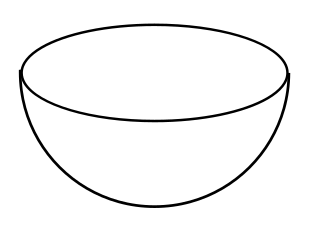
\includegraphics[width=2cm]{drawings/X1-hfhdle-01.png}
%};
%%%%%%%%%%%%%%
%\node at (0.8,-1.1) {\tiny $0^-$-hf-hdl};
%\draw[->] (1.1,0) -- (1.9,0);
%\node at (1.5,0.2) {\tiny $1^-$-hf-hdl};
%\draw[double distance=3pt] (2,-2) -- (2.3,-1.5);
%%%%%%%%%%%%%%%%%%%%%%%
%% top row, 2nd
%\node at (3,0) {
%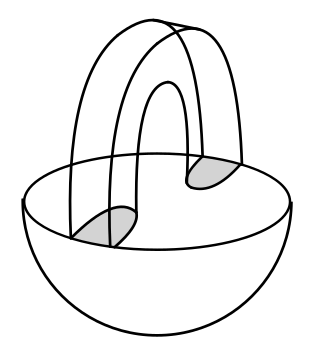
\includegraphics[width=2cm]{drawings/X1-hfhdle-02.png}
%};
%%%%%%%%%%%%%%
%\draw[->] (4.1,0) -- (4.9,0);
%\node at (4.5,0.2) {\tiny $2$-hdl};
%\draw[double distance=3pt] (5,-2) -- (5.3,-1.5);
%%%%%%%%%%%%%%%%%%%%%%%
%% bottom row, 1st
%\node at (1.5,-3.6) {
%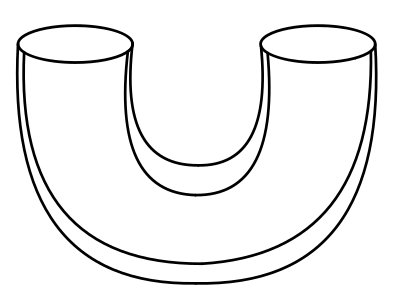
\includegraphics[width=2cm]{drawings/X1-hfhdle-03.png}
%};
%%%%%%%%%%%%%%
%\draw[->] (2.7,-3.5) -- (3.3,-3.5);
%\node at (3,-3.3) {\tiny $2$-hdl};
%%%%%%%%%%%%%%%%%%%%%%%
%% top row, 3rd
%\node at (6,0) {
%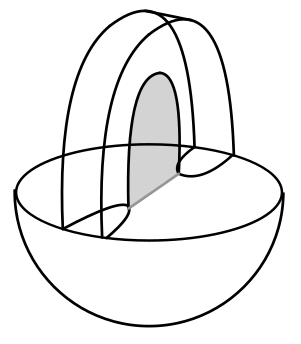
\includegraphics[width=2cm]{drawings/X1-hfhdle-04.png}
%};
%\draw[->] (7.1,0) -- (7.9,0);
%\node at (7.5,0.2) {\tiny $1$-hdl};
%%%%%%%%%%%%%%%%%%%%%%%
%% bottom row, 2nd
%\node at (4.5,-3.6) {
%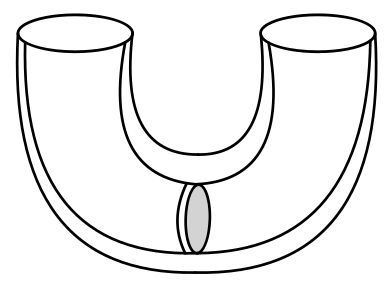
\includegraphics[width=2cm]{drawings/X1-hfhdle-05.png}
%};
%%%%%%%%%%%%%%
%\draw[double distance=3pt] (5.8,-3.5) -- (6.2,-3.5);
%%%%%%%%%%%%%%%%%%%%%%%
%% top row, 4th
%\node at (9,0) {
%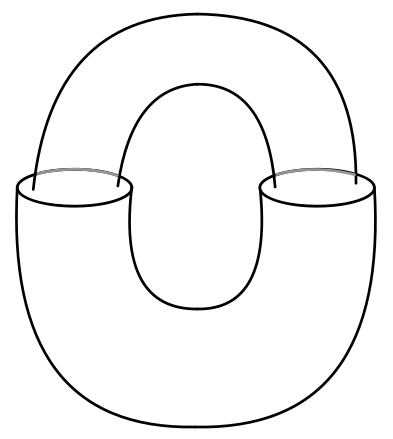
\includegraphics[width=2cm]{drawings/X1-hfhdle-06.png}
%};
%%%%%%%%%%%%%%
%\draw[->] (10.1,0) -- (10.9,0);
%\node at (10.5,0.2) {\tiny $1^+$-hf-hdl};
%%%%%%%%%%%%%%%%%%%%%%%
%% bottom row, 3rd
%\node at (7.5,-3.6) {
%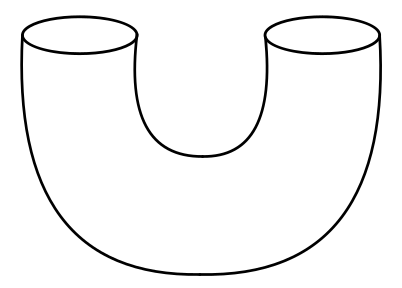
\includegraphics[width=2cm]{drawings/X1-hfhdle-07.png}
%};
%%%%%%%%%%%%%%
%\draw[->] (8.7,-3.5) -- (9.3,-3.5);
%\node at (9,-3.3) {\tiny $1^-$-hf-hdl};
%\draw[->] (7.8,-2.3) -- (8.3,-1.5);
%\node at (8.4,-1.9) {\tiny $1$-hdl};
%%%%%%%%%%%%%%%%%%%%%%%
%% top row, 5th
%\node at (12,0) {
%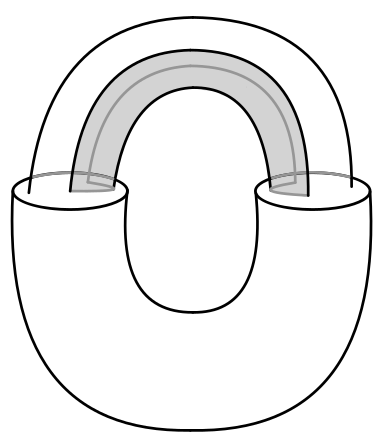
\includegraphics[width=2cm]{drawings/X1-hfhdle-08.png}
%};
%%%%%%%%%%%%%%%%%%%%%%%
%% bottom row, 4th
%\node at (10.5,-3.2) {
%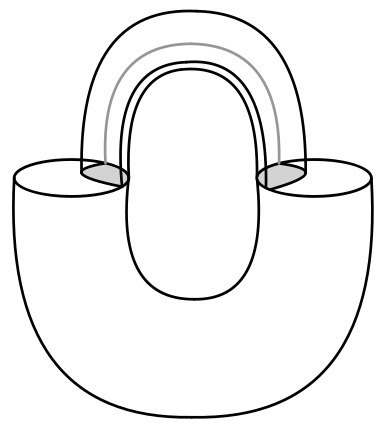
\includegraphics[width=2cm]{drawings/X1-hfhdle-09.png}
%};
%%%%%%%%%%%%%%
%\draw[double distance=3pt] (11,-2) -- (11.3,-1.5);
%\draw[->] (11.7,-3.5) -- (12.3,-3.5);
%\node at (12,-3.3) {\tiny $2^+$-hf-hdl};
%%%%%%%%%%%%%%%%%%%%%%%
%% bottom row, 5th
%\node at (13.5,-3) {
%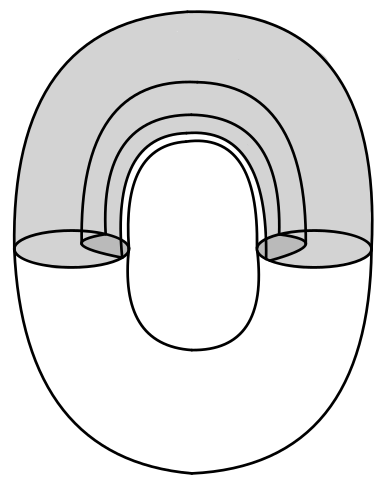
\includegraphics[width=2cm]{drawings/X1-hfhdle-10.png}
%};
%\end{tikzpicture}
%
%
%%%%%%%%%%%%%%%%%%%%%%%%%%%%%%%%%%%%%%%%%%%%%%%%%%%%%%%%%%%%%
%%%%%%%%%%%%%%%%%%%%%%%%%%%%%%%%%%%%%%%%%%%%%%%%%%%%%%%%%%%%%
%%%%%%%%%%%%%%%%%%%%%%%%%%%%%%%%%%%%%%%%%%%%%%%%%%%%%%%%%%%%%
%%%%% solid torus half-handle decomp 2
%
%\begin{tikzpicture}
%\node at (0,-0.5) {
%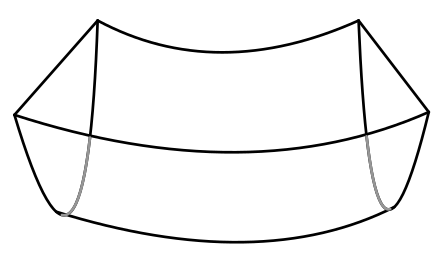
\includegraphics[width=1.5cm]{drawings/X2-hfhdle-01.png}
%};
%\node at (1.15,-0.8) {\tiny $0^-$-hf-hdl};
%\draw[->] (1,0) -- (1.8,0);
%\node at (1.4,0.2) {\tiny $1^-$-hf-hdl};
%\node at (3.5,-0.2) {
%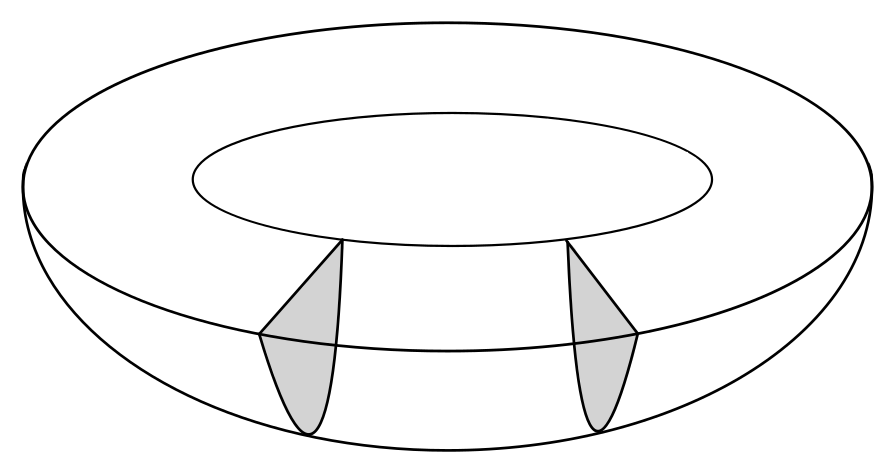
\includegraphics[width=3cm]{drawings/X2-hfhdle-02.png}
%};
%\draw[->] (5.1,0) -- (5.9,0);
%\node at (5.5,0.2) {\tiny $1^+$-hf-hdl};
%\node at (7.5,0) {
%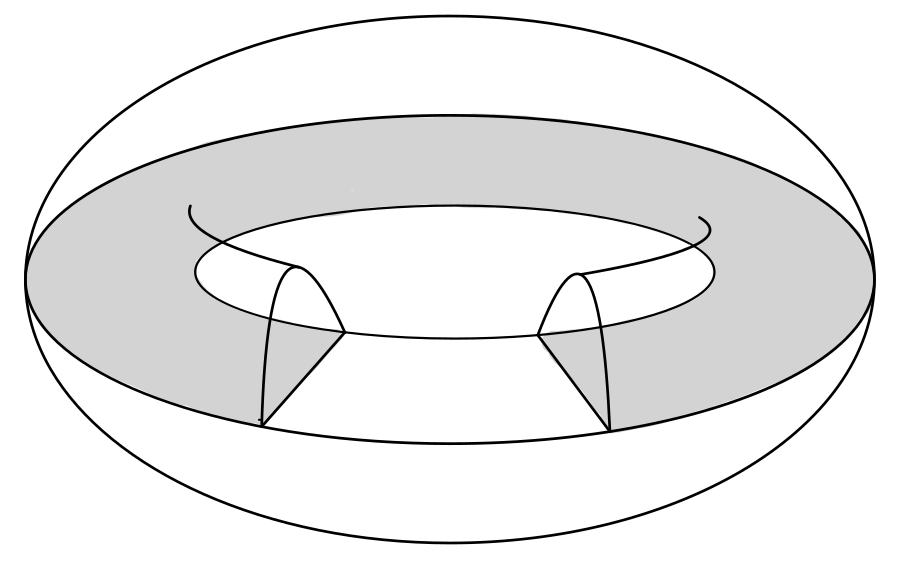
\includegraphics[width=3cm]{drawings/X2-hfhdle-03.png}
%};
%\draw[->] (9.1,0) -- (9.9,0);
%\node at  (9.5,0.2) {\tiny $2^+$-hf-hdl};
%\node at (11.5,0) {
%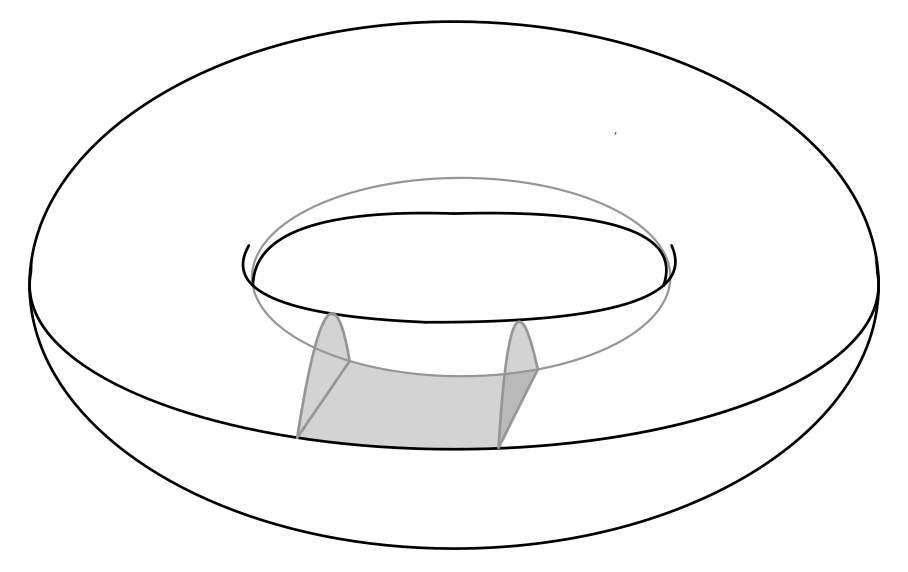
\includegraphics[width=3cm]{drawings/X2-hfhdle-04.png}
%};
%\end{tikzpicture}
%
%
%%%%%%%%%%%%%%%%%%%%%%%%%%%%%%%%%%%%%%%%%%%%%%%%%%%%%%%%%%%%%
%%%%%%%%%%%%%%%%%%%%%%%%%%%%%%%%%%%%%%%%%%%%%%%%%%%%%%%%%%%%%
%%%%%%%%%%%%%%%%%%%%%%%%%%%%%%%%%%%%%%%%%%%%%%%%%%%%%%%%%%%%%
%%%% Y-product half-handle decomp 1
%
%\begin{tikzpicture}
%\node at (0.2,0) {
%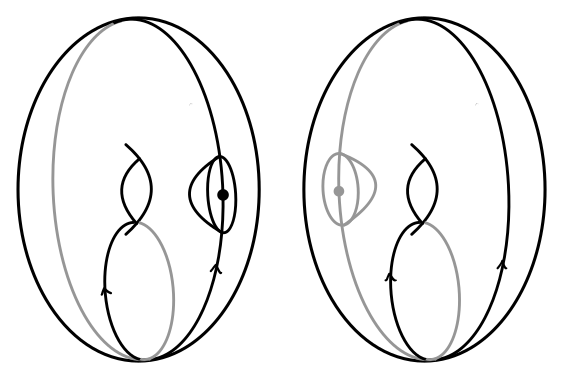
\includegraphics[width=5.5cm]{drawings/Y1-hfhdle-01-alt.png}
%};
%\draw[->] (3.2,0) -- (5.2,0);
%\node at (4.2,0.2) {\tiny $1^-$-half-handle};
%\node at (8,0) {
%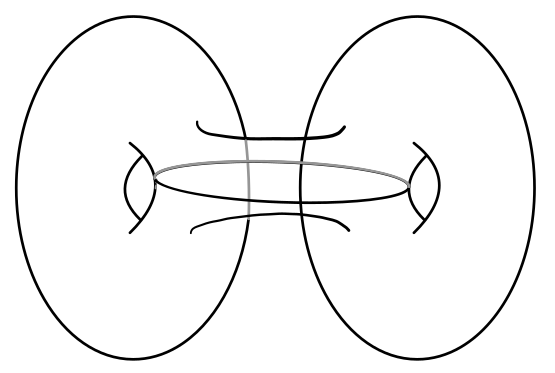
\includegraphics[width=5cm]{drawings/Y1-hfhdle-02.png}
%};
%\draw[->] (5.8,-1.8) -- (5,-2.8);
%\node at (6.4,-2.3) {\tiny $2^-$-half-handle};
%\node at (7,-5) {
%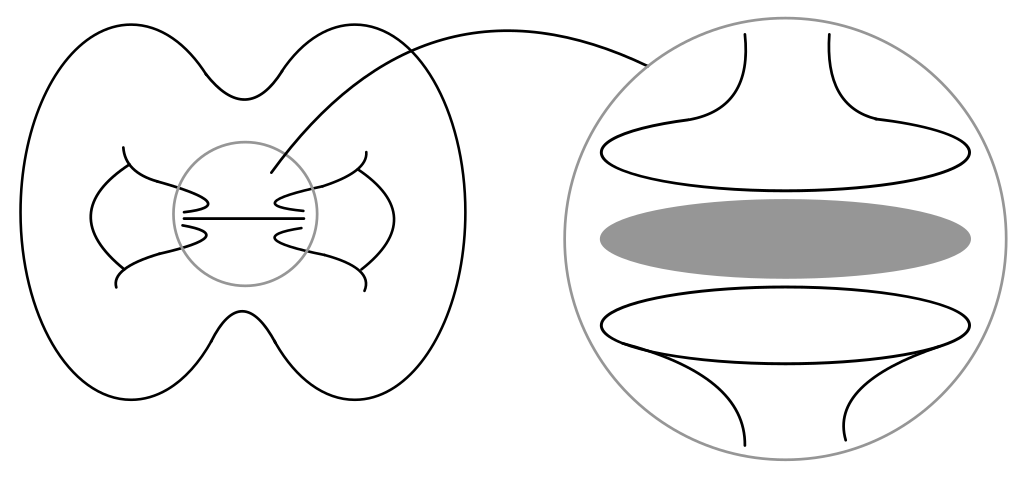
\includegraphics[width=9cm]{drawings/Y1-hfhdle-03.png}
%};
%%
%\begin{scope}[line width=0.1mm]
%\draw (6.8,-7) -- (7.8,-4.3);
%\draw (6.9,-7) -- (7.8,-5.05);
%\draw (7,-7) -- (7.8,-5.8);
%\node at (7,-7.2) {\tiny closes up};
%\node at (7,-7.4) {\tiny to a point};
%%
%\draw (4.9,-7) -- (4.7,-4.83);
%\draw (5.2,-7) -- (7.8,-5.05);
%\node at (5,-7.2) {\tiny $3$-handle};
%\node at (5,-7.4) {\tiny attaching sphere};
%\end{scope}
%%%%%%
%\node at (0,-4.8) {
%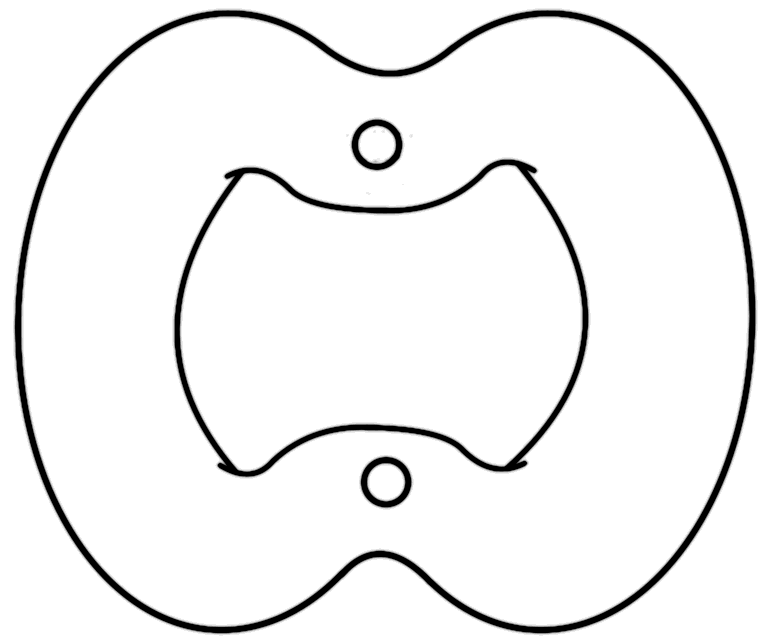
\includegraphics[width=4.2cm]{drawings/Y1-hfhdle-05-thickened-00.png}
%};
%\draw[gray] (-0.05,-3.84) circle (0.25cm);
%\draw[gray, line width=0.2mm] (-0.3,-3.84) to[out=-30,in=-150] (0.2,-3.84);
%%%%
%\node at (2.35,-4.8) {\LARGE $=$};
%%%%
%\node at (-3.5,0) {$X \sqcup X =$};
%\node at (-3.65,-4.8) {$X$};
%\draw[->] (-3.65,-0.3) -- (-3.65,-4.5);
%\node at (-3.2,-2.4) {$\mathbf{Y}_X^{(1)}$};
%\draw[->] (-2.2,-4.8) --(-3.2,-4.8);
%\node at (-2.7,-4.6) {\tiny $3$-hdl};
%\draw[line width=0.1mm] (-2.6,-4.4) -- (-2.2,-3.8) -- (-0.3,-3.8);
%\end{tikzpicture}
%
%
%%%%%%%%%%%%%%%%%%%%%%%%%%%%%%%%%%%%%%%%%%%%%%%%%%%%%%%%%%%%%
%%%%%%%%%%%%%%%%%%%%%%%%%%%%%%%%%%%%%%%%%%%%%%%%%%%%%%%%%%%%%
%%%%%%%%%%%%%%%%%%%%%%%%%%%%%%%%%%%%%%%%%%%%%%%%%%%%%%%%%%%%%
%%%%% Y-product half-handle decomp 2
%
%\begin{tikzpicture}
%\node at (0,0) {
%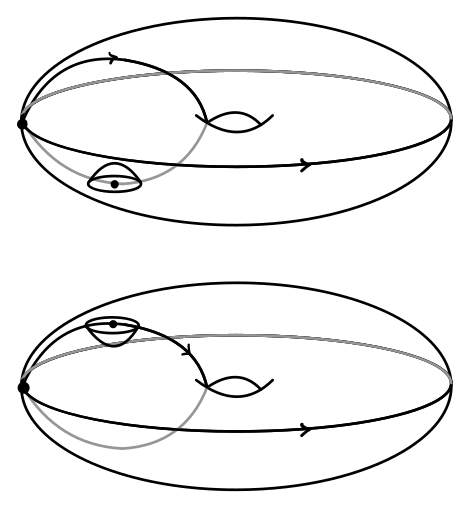
\includegraphics[width=4.2cm]{drawings/Y2-hfhdle-01.png}
%};
%\node at (5,0) {
%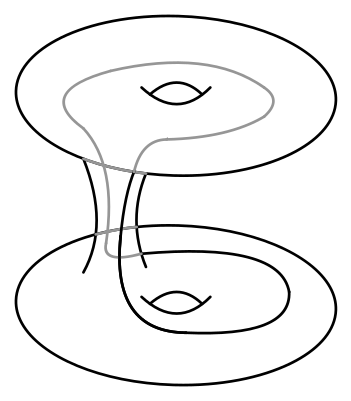
\includegraphics[width=4.2cm]{drawings/Y2-hfhdle-02.png}
%};
%%%
%\node at (-3.3,0) {$\mathbf{Y}_X^{(2)}: X \sqcup X=$};
%\node at (8.5,0) {$X$};
%\draw[->] (2,0) -- (3,0);
%\draw[->] (7,0) -- (8,0);
%\node at (2.5,0.2) {\tiny $1^-$-hf-hdl};
%\node at (7.5,0.2) {\tiny $2^-$-hf-hdl};
%\end{tikzpicture}
%
%
%%%%%%%%%%%%%%%%%%%%%%%%%%%%%%%%%%%%%%%%%%%%%%%%%%%%%%%%%%%%%
%%%%%%%%%%%%%%%%%%%%%%%%%%%%%%%%%%%%%%%%%%%%%%%%%%%%%%%%%%%%%
%%%%%%%%%%%%%%%%%%%%%%%%%%%%%%%%%%%%%%%%%%%%%%%%%%%%%%%%%%%%%
%%%%% Psi Y1 Y2 S-matrix
%
%\begin{tikzpicture}
%\node at (0,0) {
%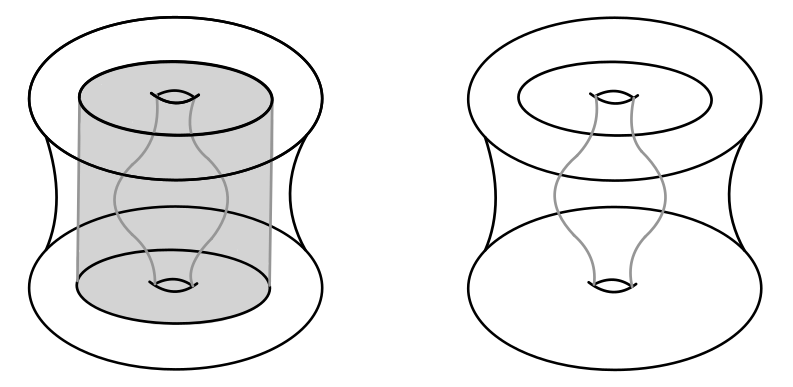
\includegraphics[width=10cm]{drawings/Psi-Y1-Y2.png}
%};
%\node at (0,0) {\LARGE $=$};
%\node at (0,2) {\small $2$-handle};
%\draw[line width=0.1mm] (-0.8,2) -- (-1.55,1.2);
%\draw[line width=0.1mm] (-0.7,1.8) -- (-0.7,-1) -- (-1.6,-1.2);
%\draw[line width=0.1mm] (0.8,2) -- (1.55,1.2);
%\node at (0,-2) {\small $3$-handle};
%\draw[line width=0.1mm] (-0.8,-2) -- (-1.6,-0.8);
%\end{tikzpicture}
%
%
%%%%%%%%%%%%%%%%%%%%%%%%%%%%%%%%%%%%%%%%%%%%%%%%%%%%%%%%%%%%%
%%%%%%%%%%%%%%%%%%%%%%%%%%%%%%%%%%%%%%%%%%%%%%%%%%%%%%%%%%%%%
%%%%%%%%%%%%%%%%%%%%%%%%%%%%%%%%%%%%%%%%%%%%%%%%%%%%%%%%%%%%%
%%%%% relative cobord to cornered cobord
%
%\begin{tikzpicture}
%\node at (0,0) {
%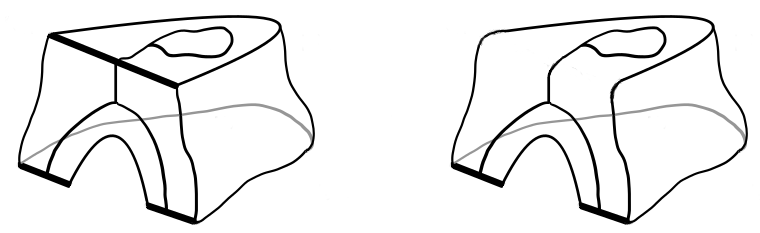
\includegraphics[width=10cm]{drawings/relative-to-corner-cobordism-alt.png}
%};
%%% left side
%\node at (-4.8,1.2) {$N_-$};
%\node at (-5,-0.8) {$N_+$};
%\node at (-5,0.2) {$M$};
%\node at (-0.8,0.4) {$W$};
%\node at (-0.5,-0.4) {$M_+$};
%\node at (-0.9,1.2) {$M_-$};
%\node at (-1.7,1.1) {\small $\varphi_-$};
%\node at (-3.7,0.4) {\small $\varphi$};
%%% right side
%\begin{scope}[shift={(5.7,0)}]
%\node at (-5,-0.8) {$N_+$};
%\node at (-0.8,0.4) {$W$};
%\node at (-0.5,-0.4) {$M_+$};
%\node at (-0.5,1.2) {$M \cup M_-$};
%\node[rotate=50] at (-3.9,0.4) {\small $\varphi \cup \varphi_-$};
%\end{scope}
%\end{tikzpicture}

%%%%%%%%%%%%%%%%%%%%%%%%%%%%%%%%%%%%%%%%%%%%%%%%%%%%%%%%%%%%%
%%%%%%%%%%%%%%%%%%%%%%%%%%%%%%%%%%%%%%%%%%%%%%%%%%%%%%%%%%%%%
%%%%%%%%%%%%%%%%%%%%%%%%%%%%%%%%%%%%%%%%%%%%%%%%%%%%%%%%%%%%%
%%%%% Psi skein
%
%\begin{tikzpicture}
%\node at (-2.1,0) {$\varphi_j =$};
%%%% first
%\draw (0,0) ellipse (1.5cm and 1cm);
%\draw (-0.2,0.1) to[out=-60,in=-120] (0.2,0.1);
%\draw (-0.1,0) to[out=60,in=120] (0.1,0);
%% skein
%\draw[midarrow={0.8}] (0,0) ellipse (0.8cm and 0.5cm);
%\node at (0.3,-0.6) {\tiny $j$};
%% label
%\node at (1.3,-0.9) {$X$};
%%%%%%%%%%%%%%%%%%%%%
%\draw[|->] (1.8,0) -- (3.2,0);
%\node at (2.5,0.3) {\small 2-handle};
%%%%%%%%%%%%%%%%%%%%%
%%%% second
%\begin{scope}[shift={(5,0)}]
%\draw (0,0) ellipse (1.5cm and 1cm);
%\draw (-0.2,0.1) to[out=-60,in=-120] (0.2,0.1);
%\draw (-0.1,0) to[out=60,in=120] (0.1,0);
%%% handle and Omega
%\draw (0,0) ellipse (0.6cm and 0.4cm);
%\draw[thin_overline={2},dashed] (-0.6,0) circle (0.2cm);
%\draw[thin_overline={1}] (-0.6,0) arc (180:360:0.6cm and 0.4cm);
%% skein
%\draw[midarrow={0.8}] (0,0) ellipse (1.2cm and 0.8cm);
%\node at (0.1,-0.65) {\tiny $j$};
%% label
%\node at (1.3,-0.9) {$X'$};
%\draw[line width=0.1mm] (-1.9,0.5) -- (-1.3,0.9) -- (-0.2,0.38);
%\end{scope}
%%%%%%%%%%%%%%%%%%%%%
%\draw[|->] (6.8,0) -- (8.2,0);
%\node at (7.65,0.7) {$m \mapsto l$};
%\node at (7.8,0.3) {$l \mapsto -m$};
%\node at (6.8,0.5) {$\Psi:$};
%%%%%%%%%%%%%%%%%%%%%
%%%% third
%\begin{scope}[shift={(10,0)}]
%\draw (0,0) ellipse (1.5cm and 1cm);
%\draw (-0.2,0.1) to[out=-60,in=-120] (0.2,0.1);
%\draw (-0.1,0) to[out=60,in=120] (0.1,0);
%%% skein
%\draw[dashed] (0,0) ellipse (0.8cm and 0.5cm);
%\draw[thin_overline={1}] (-0.8,0) circle (0.2cm);
%\draw[dashed,thin_overline={2}] (-0.8,0) arc (180:360:0.8cm and 0.5cm);
%\node at (-1.2,0) {\tiny $j$};
%\draw[->] (-1,0.05) -- (-1,-0.05);
%% label
%\node at (1.3,-0.9) {$X$};
%\end{scope}
%%%%%%%%%%%%%%%%%%%%%
%\node at (12.5,0) {$= \sum s_{ij} \varphi_i$};
%\end{tikzpicture}
%
%
%%%%%%%%%%%%%%%%%%%%%%%%%%%%%%%%%%%%%%%%%%%%%%%%%%%%%%%%%%%%%
%%%%%%%%%%%%%%%%%%%%%%%%%%%%%%%%%%%%%%%%%%%%%%%%%%%%%%%%%%%%%
%%%%%%%%%%%%%%%%%%%%%%%%%%%%%%%%%%%%%%%%%%%%%%%%%%%%%%%%%%%%%
%%%%% Y2 skein
%
%\begin{tikzpicture}
%\node at (-3.6,0) {$Z_{CY}(\mathbf{Y}_X^{(2)})(\varphi_i \otimes \varphi_j) =$};
%%%%%%%%%%%%%%%%%%%%%%%%%%
%\draw (0,0) ellipse (1.5cm and 1cm);
%\draw (-0.2,0.1) to[out=-60,in=-120] (0.2,0.1);
%\draw (-0.1,0) to[out=60,in=120] (0.1,0);
%%% skein
%\draw[midarrow={0.7}] (0,-0.2) ellipse (0.8cm and 0.5cm);
%\draw[thin_overline={2},midarrow={0.7}] (0,0.2) ellipse (0.8cm and 0.5cm);
%\node at (-0.2,-0.4) {\tiny $i$};
%\node at (-0.2,-0.82) {\tiny $j$};
%%%%%%%%%%%%%%%%%%%%%%%%%%
%\node at (1.8,0) {$=$};
%%%%%%%%%%%%%%%%%%%%%%%%%%
%%%%% second
%\begin{scope}[shift={(3.6,0)}]
%\draw (0,0) ellipse (1.5cm and 1cm);
%\draw (-0.2,0.1) to[out=-60,in=-120] (0.2,0.1);
%\draw (-0.1,0) to[out=60,in=120] (0.1,0);
%%% skein
%\draw (-1.1,0) arc (180:40:1.1cm and 0.7cm);
%\draw[midarrow={0.5}] (-1.1,0) arc (180:320:1.1cm and 0.7cm);
%\draw (-0.8,0) arc (180:40:0.8cm and 0.5cm);
%\draw[midarrow={0.4}] (-0.8,0) arc (180:320:0.8cm and 0.5cm);
%\node at (-0.2,-0.36) {\tiny $j$};
%\node at (-0.2,-0.82) {\tiny $i$};
%\node[dotnode] (a1) at (0.9,0.2) {};
%\node[dotnode] (a2) at (0.9,-0.2) {};
%\node at (1.1,0.2) {\tiny $\alpha$};
%\node at (1.1,-0.2) {\tiny $\alpha$};
%\draw (a1) to[out=90,in=-30] (0.83,0.46);
%\draw (a1) to[out=150,in=-30] (0.6,0.33);
%\draw (a2) to[out=-90,in=30] (0.83,-0.46);
%\draw (a2) to[out=-150,in=30] (0.6,-0.33);
%\draw[dotted] (a1) to[out=-60,in=60] (a2);
%\end{scope}
%%%%%%%%%%%%%%%%%%%%%%%%%%
%\node at (5.4,0) {$=$};
%%%%%%%%%%%%%%%%%%%%%%%%%%
%%%%% third
%\begin{scope}[shift={(7.2,0)}]
%\draw (0,0) ellipse (1.5cm and 1cm);
%\draw (-0.2,0.1) to[out=-60,in=-120] (0.2,0.1);
%\draw (-0.1,0) to[out=60,in=120] (0.1,0);
%%% skein
%\draw[dashed] (0.8,0) arc (0:140:0.8cm and 0.5cm);
%\draw[dashed] (0.8,0) arc (0:-140:0.8cm and 0.5cm);
%\draw[white, line width=0.8mm] (0.78,0) -- (0.82,0);
%\node[dotnode] (a3) at (-0.6,0.33) {};
%\node[dotnode] (a4) at (-0.6,-0.33) {};
%\node at (-0.74,0.4) {\tiny $\alpha$};
%\node at (-0.74,-0.4) {\tiny $\alpha$};
%\draw[midarrow] (a3) to[out=-150,in=150] (a4);
%\draw[midarrow] (a3) to[out=-70,in=70] (a4);
%\node at (-0.9,0) {\tiny $i$};
%\node at (-0.4,0) {\tiny $j$};
%\end{scope}
%%%%%%%%%%%%%%%%%%%%%%%%%%
%\node at (9.7,0) {$= \sum N_{ij}^k \varphi_k$};
%\end{tikzpicture}
%
%
%%%%%%%%%%%%%%%%%%%%%%%%%%%%%%%%%%%%%%%%%%%%%%%%%%%%%%%%%%%%%
%%%%%%%%%%%%%%%%%%%%%%%%%%%%%%%%%%%%%%%%%%%%%%%%%%%%%%%%%%%%%
%%%%%%%%%%%%%%%%%%%%%%%%%%%%%%%%%%%%%%%%%%%%%%%%%%%%%%%%%%%%%
%%%%% Y1 skein
%
%\begin{tikzpicture}
%\node at (-4,0) {$\varphi_i \otimes \varphi_j$};
%\draw[|->] (-3,0) -- (-2,0);
%\node at (-2.5,0.7) {\small $1^-$-,$2^-$-};
%\node at (-2.5,0.3) {\small hf-hdl};
%%%%%%%%%%%%%%%%%%%%%%%%%
%\node at (0,0) {
%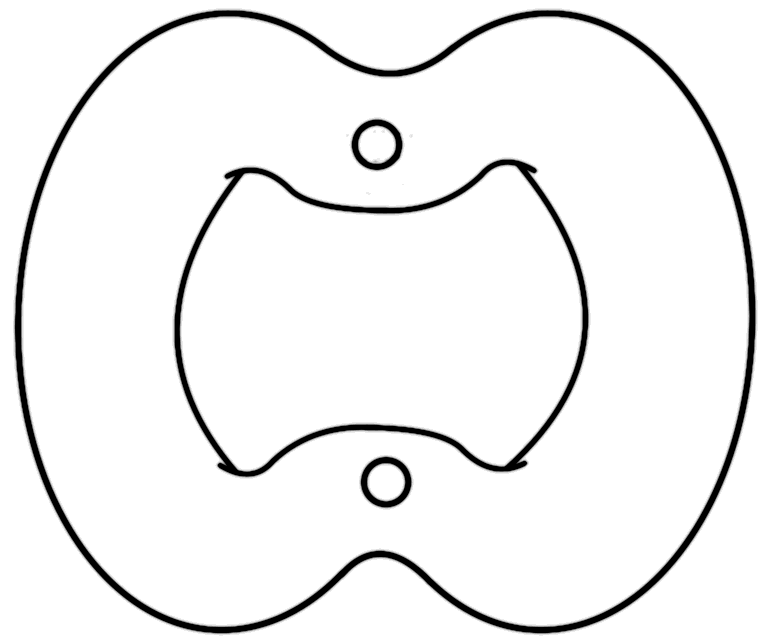
\includegraphics[width=3cm]{drawings/Y1-hfhdle-05-thickened-00.png}
%};
%\draw (0.06,0.7) .. controls +(20:0.5cm) and +(90:1cm) ..
%	(1.1,0);
%\draw[midarrow={0.99}] (0.09,-0.67) .. controls +(-20:0.5cm) and +(-90:1cm) ..
%	(1.1,0);
%\draw[midarrow={0.99}] (-0.11,0.7) .. controls +(160:0.5cm) and +(90:1cm) ..
%	(-1.1,0);
%\draw (-0.09,-0.67) .. controls +(-160:0.5cm) and +(-90:1cm) ..
%	(-1.1,0);
%\node at (-1.25,0) {\tiny $i$};
%\node at (1.25,0.1) {\tiny $j$};
%%%%%%%%%%%%%%%%%%%%%%%%
%\draw[|->] (1.75,0) -- (2.75,0);
%\node at (2.25,0.3) {\small 3-hdl};
%%%%%%%%%%%%%%%%%%%%%%%%
%\begin{scope}[shift={(4.5,0)}]
%\node at (0,0) {
%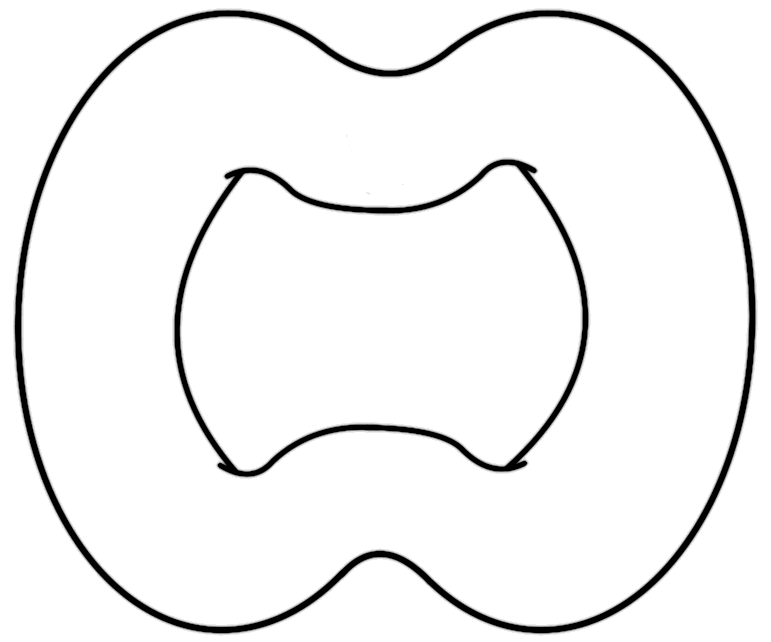
\includegraphics[width=3cm]{drawings/Y1-hfhdle-05-no-circles.png}
%};
%\node[dotnode] (a1) at (0,0.7) {};
%\node[dotnode] (a2) at (0,-0.7) {};
%\node at (0,0.58) {\tiny $\alpha$};
%\node at (0,-0.58) {\tiny $\alpha$};
%\draw (a1) .. controls +(20:0.5cm) and +(90:1cm) ..
%	(1.1,0);
%\draw[midarrow={0.99}] (a2) .. controls +(-20:0.5cm) and +(-90:1cm) ..
%	(1.1,0);
%\draw[midarrow={0.99}] (a1) .. controls +(160:0.5cm) and +(90:1cm) ..
%	(-1.1,0);
%\draw (a2) .. controls +(-160:0.5cm) and +(-90:1cm) ..
%	(-1.1,0);
%\node at (-1.25,0) {\tiny $i$};
%\node at (1.25,0.1) {\tiny $j$};
%\end{scope}
%%%%%%%%%%%%%%%%%%%%%%%%
%\node at (7,0) {$= \frac{\delta_{ij}}{d_i} \cdot \varphi_i$};
%\end{tikzpicture}
%
%
%%%%%%%%%%%%%%%%%%%%%%%%%%%%%%%%%%%%%%%%%%%%%%%%%%%%%%%%%%%%%
%%%%%%%%%%%%%%%%%%%%%%%%%%%%%%%%%%%%%%%%%%%%%%%%%%%%%%%%%%%%%
%%%%%%%%%%%%%%%%%%%%%%%%%%%%%%%%%%%%%%%%%%%%%%%%%%%%%%%%%%%%%
%%%%% K Psi Psi
%
%\begin{tikzpicture}
%\node at (-3.5,0) {$K := \Psi \circ \overline{\Psi} =
%\overline{\Psi} \circ \Psi =$};
%%%%%%%%%
%\draw (0,0) ellipse (1.5cm and 1cm);
%\draw (-0.2,0.1) to[out=-60,in=-120] (0.2,0.1);
%\draw (-0.1,0) to[out=60,in=120] (0.1,0);
%%%%%%%%%
%\draw (0,0) ellipse (0.8cm and 0.5cm);
%\draw[overline] (-0.8,0) circle (0.2cm);
%\draw[overline] (0.8,0) arc (0:-180:0.8cm and 0.5cm);
%%% label
%\node at (-2,0.8) {\tiny 2-handle};
%\draw[line width=0.1mm] (-1.5,0.6) -- (-1,0.1);
%\draw[line width=0.1mm] (-1.4,0.8) -- (-0.5,0.4);
%\end{tikzpicture}
%
%
%
%%%%%%%%%%%%%%%%%%%%%%%%%%%%%%%%%%%%%%%%%%%%%%%%%%%%%%%%%%%%%
%%%%%%%%%%%%%%%%%%%%%%%%%%%%%%%%%%%%%%%%%%%%%%%%%%%%%%%%%%%%%
%%%%%%%%%%%%%%%%%%%%%%%%%%%%%%%%%%%%%%%%%%%%%%%%%%%%%%%%%%%%%
%%%%% Y2 Psi Psi
%
%\begin{tikzpicture}[scale=0.9]
%\begin{scope}[shift={(-3,0)}]
%\node at (-4.4,0) {$X \sqcup X$};
%\draw[->] (-3.5,0) -- (-2.5,0);
%\node at (-3,0.3) {$\Psi \sqcup \Psi$};
%%% left X
%\begin{scope}[shift={(-1.2,0)}];
%\draw (0,0) ellipse (1cm and 1.7cm);
%\draw (-0.1,-0.2) to[out=30,in=-30] (-0.1,0.2);
%\draw (0,-0.1) to[out=150,in=-150] (0,0.1);
%\draw (0,0) ellipse (0.5cm and 0.8cm);
%\end{scope}
%%% right X
%\begin{scope}[shift={(1,0)}];
%\draw (0,0) ellipse (1cm and 1.7cm);
%\draw (-0.1,-0.2) to[out=30,in=-30] (-0.1,0.2);
%\draw (0,-0.1) to[out=150,in=-150] (0,0.1);
%\draw (0,0) ellipse (0.5cm and 0.8cm);
%\end{scope}
%%%%%%%%%%%%%%%%%
%\draw[->] (2.3,0) -- (3.5,0);
%\node at (2.9,0.4) {$\mathbf{Y}_X^{(2)}$};
%%%%%%%%%%%%%%%%%
%\begin{scope}[shift={(5.8,0)}]
%\node at (0,0) {
%% 4.2cm * 0.9 = 3.78cm
%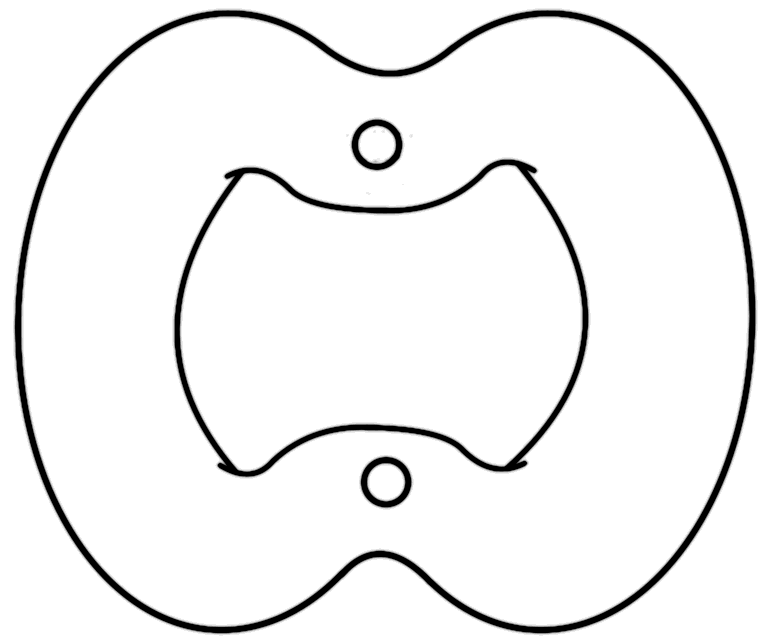
\includegraphics[width=3.78cm]{drawings/Y1-hfhdle-05-thickened-00.png}
%};
%%% 2-handles
%\draw (-0.15,1.05)
%	.. controls +(135:0.2cm) and +(45:0.4cm) .. (-1.2,1.0)
%	.. controls +(-135:0.4cm) and +(90:0.4cm) .. (-1.5,0)
%	.. controls +(-90:0.4cm) and +(135:0.4cm) .. (-1.2,-1)
%	.. controls +(-45:0.4cm) and +(-135:0.4cm) .. (-0.1,-0.9);
%\draw (0.05,1.05)
%	.. controls +(45:0.2cm) and +(135:0.4cm) .. (1.2,1.0)
%	.. controls +(-45:0.4cm) and +(90:0.4cm) .. (1.5,0)
%	.. controls +(-90:0.4cm) and +(45:0.4cm) .. (1.2,-1)
%	.. controls +(-135:0.4cm) and +(-45:0.4cm) .. (0.1,-0.95);
%\end{scope}
%%%%%%%%%%%%%%%%%
%\node at (8.4,0) {$=$};
%%%%%%%%%%%%%%%%%
%%% final X
%\begin{scope}[shift={(10,0)}];
%\draw (0,0) ellipse (1cm and 1.7cm);
%\draw (-0.1,-0.2) to[out=30,in=-30] (-0.1,0.2);
%\draw (0,-0.1) to[out=150,in=-150] (0,0.1);
%\draw (0,0) ellipse (0.5cm and 0.8cm);
%\end{scope}
%\end{scope}
%\end{tikzpicture}
%
%%%%%%%%%%%%%%%%%%%%%%%%%%%%%%%%%%%%%%%%%%%%%%%%%%%%%%%%%%%%%
%%%%%%%%%%%%%%%%%%%%%%%%%%%%%%%%%%%%%%%%%%%%%%%%%%%%%%%%%%%%%
%%%%%%%%%%%%%%%%%%%%%%%%%%%%%%%%%%%%%%%%%%%%%%%%%%%%%%%%%%%%%
%%%%% K Psi Y1
%
%\begin{tikzpicture}[scale=0.9]
%\begin{scope}[shift={(-3,0)}]
%\node at (-4.4,0) {$X \sqcup X$};
%\draw[->] (-3.5,0) -- (-2.5,0);
%\node at (-3,0.3) {$K \sqcup \text{id}$};
%%% left X
%\begin{scope}[shift={(-1.2,0)}];
%\draw (0,0) ellipse (1cm and 1.7cm);
%\draw (-0.1,-0.2) to[out=30,in=-30] (-0.1,0.2);
%\draw (0,-0.1) to[out=150,in=-150] (0,0.1);
%\draw (0,0) ellipse (0.5cm and 0.8cm);
%\draw[overline] (0.38,0.5) circle (0.15cm);
%\draw[overline] (0,-0.8) arc (-90:40:0.5cm and 0.8cm);
%\end{scope}
%%% right X
%\begin{scope}[shift={(1,0)}];
%\draw (0,0) ellipse (1cm and 1.7cm);
%\draw (-0.1,-0.2) to[out=30,in=-30] (-0.1,0.2);
%\draw (0,-0.1) to[out=150,in=-150] (0,0.1);
%\end{scope}
%%%%%%%%%%%%%%%%%
%\draw[->] (2.3,0) -- (3.5,0);
%\node at (2.9,0.4) {$\mathbf{Y}_X^{(1)}$};
%%%%%%%%%%%%%%%%%
%\begin{scope}[shift={(5.8,0)}]
%\node at (0,0) {
%% 4.2cm * 0.9 = 3.78cm
%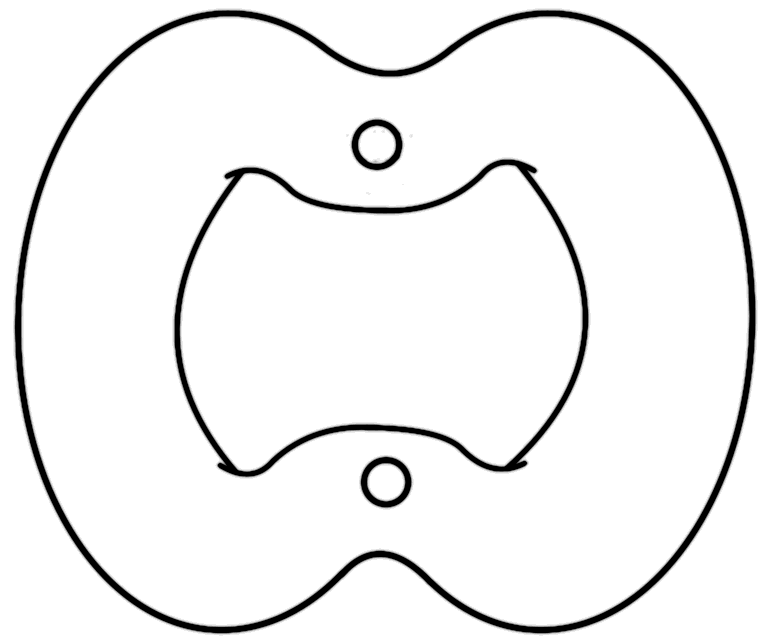
\includegraphics[width=3.78cm]{drawings/Y1-hfhdle-05-thickened-00.png}
%};
%\draw[gray] (-0.05,0.96) circle (0.3cm);
%\draw[gray, line width=0.2mm] (-0.35,0.96) to[out=-30,in=-150] (0.25,0.96);
%%% 2-handles from K
%% small one
%\draw (-0.18,1.18) .. controls +(45:0.1cm) and +(45:0.2cm) ..
%	(-0.18,1.08);
%\draw (-0.28,1.08) .. controls +(-135:0.1cm) and +(-135:0.2cm) ..
%	(-0.18,1.08);
%% long one
%\draw[thin_overline={1}] (-0.22,1.12)
%	.. controls +(135:0.2cm) and +(45:0.4cm) .. (-1.2,1.0);
%\draw (-1.2,1)
%	.. controls +(-135:0.4cm) and +(90:0.4cm) .. (-1.5,0)
%	.. controls +(-90:0.4cm) and +(135:0.4cm) .. (-1.2,-1)
%	.. controls +(-45:0.4cm) and +(-135:0.4cm) .. (-0.1,-0.9);
%\end{scope}
%%%%%%%%%%%%%%%%%
%\node at (8.2,0) {$=$};
%%%%%%%%%%%%%%%%%
%\begin{scope}[shift={(10.6,0)}]
%\node at (0,0) {
%% 4.2cm * 0.9 = 3.78cm
%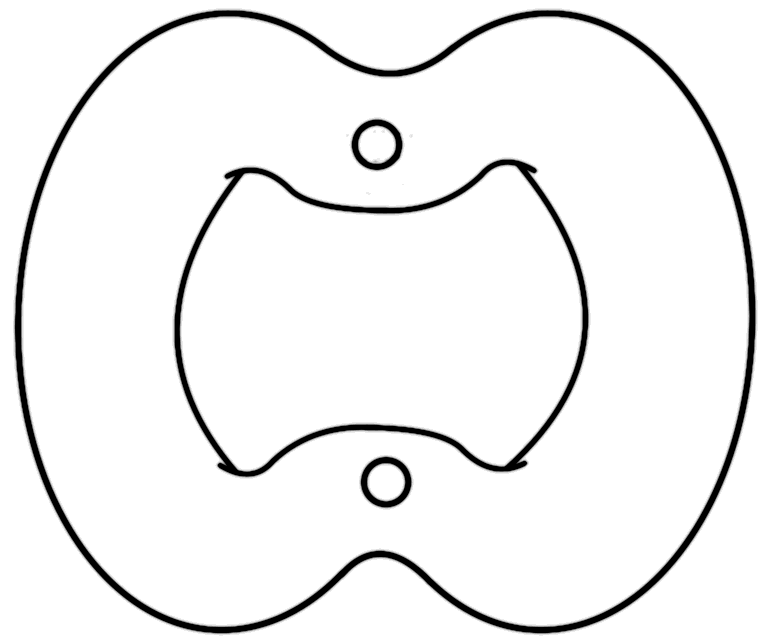
\includegraphics[width=3.78cm]{drawings/Y1-hfhdle-05-thickened-00.png}
%};
%%% 2-handle
%% long one
%\draw (-0.15,1.05)
%	.. controls +(135:0.2cm) and +(45:0.4cm) .. (-1.2,1.0)
%	.. controls +(-135:0.4cm) and +(90:0.4cm) .. (-1.5,0)
%	.. controls +(-90:0.4cm) and +(135:0.4cm) .. (-1.2,-1)
%	.. controls +(-45:0.4cm) and +(-135:0.4cm) .. (-0.1,-0.9);
%\end{scope}
%%%%%%%%%%%%%%%%%
%\node at (13.1,0) {$= X$};
%\end{scope}
%\end{tikzpicture}
%
%%%%%%%%%%%%%%%%%%%%%%%%%%%%%%%%%%%%%%%%%%%%%%%%%%%%%%%%%%%%%
%%%%%%%%%%%%%%%%%%%%%%%%%%%%%%%%%%%%%%%%%%%%%%%%%%%%%%%%%%%%%
%%%%%%%%%%%%%%%%%%%%%%%%%%%%%%%%%%%%%%%%%%%%%%%%%%%%%%%%%%%%%
%%%%% counit Y1
%
%\begin{tikzpicture}
%\node at (-3.5,0) {$X$};
%\draw[->, line width=0.3mm] (-3.0,0) -- (-1.7,0);
%\node at (-2.4,0.25) {\scriptsize $2^-$-hf-hdl};
%%%%
%\draw (0,0) ellipse (1.5cm and 1cm);
%\draw (-0.4,0.1) to[out=-60,in=-120] (0.4,0.1);
%\draw (-0.29,0) to[out=60,in=120] (0.29,0);
%\draw[fill=black,opacity=0.2] (0,0) ellipse (0.3cm and 0.2cm);
%% line labeling 2 handle
%\draw[line width=0.1mm] (-2,0.5) -- (-1.8,0.8) -- (0,0);
%%%%
%\node at (3.8,0.1) {$= \mathcal{D}^3
%\xrightarrow{3^- \text{-hf-hdl}}
%S^3
%\xrightarrow{4 \text{-hdl}}
%\emptyset
%$};
%\draw[->, line width=0.3mm] (2.3,-0.3) to[out=-30,in=-150] (5.5,-0.3);
%\node at (3.9,-0.95) {\scriptsize $3^+$-hf-hdl};
%\end{tikzpicture}
%
%%%%%%%%%%%%%%%%%%%%%%%%%%%%%%%%%%%%%%%%%%%%%%%%%%%%%%%%%%%%%
%%%%%%%%%%%%%%%%%%%%%%%%%%%%%%%%%%%%%%%%%%%%%%%%%%%%%%%%%%%%%
%%%%%%%%%%%%%%%%%%%%%%%%%%%%%%%%%%%%%%%%%%%%%%%%%%%%%%%%%%%%%
%%%%% counit Y2
%
%\begin{tikzpicture}
%\node at (-2.2,0) {$X =$};
%%%%%%%%%%%%%%%%%%%%
%\draw (0,0) ellipse (1.5cm and 1cm);
%\draw (-0.4,0.1) to[out=-60,in=-120] (0.4,0.1);
%\draw (-0.29,0) to[out=60,in=120] (0.29,0);
%%% the 2+ half-handle
%%\draw[fill=black,opacity=0.2] (0,0.57) ellipse (0.1cm and 0.42cm);
%%\draw[fill=black,opacity=0.2] (0.1,0.57) ellipse (0.1cm and 0.42cm);
%\draw[fill=black,opacity=0.2] (0,1)
%	.. controls +(-150:0.1cm) and +(90:0.2cm) .. (-0.1,0.55)
%	.. controls +(-90:0.2cm) and +(150:0.1cm) .. (0,0.15)
%	-- (0.1,0.15)
%	.. controls +(30:0.1cm) and +(-90:0.2cm) .. (0.2,0.55)
%	.. controls +(90:0.2cm) and +(-30:0.1cm) .. (0.1,1);
%\draw[opacity=0.2] (0.1,0.15)
%	.. controls +(150:0.1cm) and +(-90:0.2cm) .. (0,0.55)
%	.. controls +(90:0.2cm) and +(-150:0.1cm) .. (0.1,1);
%%%%%%%%%%%%%%%%%%%%
%\node at (3.7,0) {
%$\xrightarrow{2^+ \text{-hf-hdl}}
%\mathcal{D}^3
%\xrightarrow{3^+ \text{-hf-hdl}}
%\emptyset
%$};
%%%%%%%%%%%%%%%%%%%%
%\draw[line width=0.1mm] (0.1,0.55) -- (1.6,0.8) -- (1.8,0.4);
%\end{tikzpicture}
%
%%%%%%%%%%%%%%%%%%%%%%%%%%%%%%%%%%%%%%%%%%%%%%%%%%%%%%%%%%%%%
%%%%%%%%%%%%%%%%%%%%%%%%%%%%%%%%%%%%%%%%%%%%%%%%%%%%%%%%%%%%%
%%%%%%%%%%%%%%%%%%%%%%%%%%%%%%%%%%%%%%%%%%%%%%%%%%%%%%%%%%%%%
%%%%% higher genus skein basis
%
%\begin{tikzpicture}
%\begin{scope}[shift={(-3,0)}]
%\node[small_morphism,minimum size=5pt] (ph) at (0,0) {\scriptsize $\varphi$};
%\draw (ph) to[out=150,in=-90] (-0.45,0.6);
%\draw (ph) to[out=-150,in=90] (-0.45,-0.6);
%\draw (ph) to[out=110,in=-90] (-0.15,0.6);
%\draw (ph) to[out=-110,in=90] (-0.15,-0.6);
%\draw (ph) to[out=70,in=-90] (0.15,0.6);
%\draw (ph) to[out=-70,in=90] (0.15,-0.6);
%\draw (ph) to[out=30,in=-90] (0.45,0.6);
%\draw (ph) to[out=-30,in=90] (0.45,-0.6);
%\draw (ph) to[out=180,in=-90] (-0.9,0.6);
%% labels
%\node at (-0.9,0.8) {\scriptsize $A$};
%\node at (-0.45,0.8) {\scriptsize $i_1$};
%\node at (-0.45,-0.8) {\scriptsize $i_1$};
%\node at (-0.15,0.8) {\scriptsize $i_2$};
%\node at (-0.15,-0.8) {\scriptsize $i_2$};
%\node at (0.15,0.8) {\scriptsize $i_3$};
%\node at (0.15,-0.8) {\scriptsize $i_3$};
%\node at (0.45,0.8) {\scriptsize $i_4$};
%\node at (0.45,-0.8) {\scriptsize $i_4$};
%\end{scope}
%%%%%%%%%%%%%%%%%%%%%
%\node at (-2,0) {$\mapsto$};
%%%%%%%%%%%%%%%%%%%%%
%\draw (0,0) ellipse (1.5cm and 1cm);
%\draw (-0.4,0.1) to[out=-60,in=-120] (0.4,0.1);
%\draw (-0.29,0) to[out=60,in=120] (0.29,0);
%\node[fill=black,circle,inner sep=2pt,outer sep=0pt] (d1) at (0.35,0.01) {};
%%
%\node[small_morphism,minimum size=5pt] (p1) at (-0.7,0) {\scriptsize $\varphi$};
%%\node[dotnode,inner sep=1.5pt] (p1) at (-0.7,0) {};
%\draw[midarrow_rev] (p1) -- (-1.5,0);
%\node at (-1.2,0.2) {\tiny $A$};
%%\node at (-0.5,0) {\tiny $\varphi$};
%%% label for the boundary point
%\node at (0,-1.3) {\scriptsize $(1/2,1/2)$};
%\draw[line width=0.1mm] (0,-1.1) -- (d1);
%%%% line connecting above label to the next label
%\draw[line width=0.1mm,dashed] (0.7,-1.3) -- (3.1,-1.3);
%% i1 strand
%\draw (p1) .. controls +(150:0.5cm) and +(180:0.9cm) ..
%	(0,0.8);
%\draw (p1) .. controls +(-150:0.5cm) and +(180:0.9cm) ..
%	(0,-0.8);
%\draw[midarrow_rev] (0,0.8) arc (90:-90:1.3cm and 0.8cm);
%\node at (1.15,0) {\tiny $i_1$};
%% i2 strand
%\draw (p1) .. controls +(110:0.4cm) and +(180:0.7cm) ..
%	(0,0.65);
%\draw (p1) .. controls +(-110:0.4cm) and +(180:0.7cm) ..
%	(0,-0.65);
%\draw (0.35,0) .. controls +(10:0.8cm) and +(0:0.8cm) ..
%	(0,0.65);
%\draw (0.35,0) .. controls +(-10:0.8cm) and +(0:0.8cm) ..
%	(0,-0.65);
%% i3 strand
%\draw (p1) .. controls +(70:0.3cm) and +(180:0.6cm) ..
%	(0,0.5);
%\draw (p1) .. controls +(-70:0.3cm) and +(180:0.6cm) ..
%	(0,-0.5);
%\draw (0.35,0) .. controls +(30:0.5cm) and +(0:0.6cm) ..
%	(0,0.5);
%\draw (0.35,0) .. controls +(-30:0.5cm) and +(0:0.6cm) ..
%	(0,-0.5);
%% i4 strand
%\draw (p1) .. controls +(30:0.2cm) and +(180:0.5cm) ..
%	(0,0.35);
%\draw (p1) .. controls +(-30:0.2cm) and +(180:0.5cm) ..
%	(0,-0.35);
%\draw (0.35,0) .. controls +(60:0.3cm) and +(0:0.4cm) ..
%	(0,0.35);
%\draw (0.35,0) .. controls +(-60:0.3cm) and +(0:0.4cm) ..
%	(0,-0.35);
%%%%%%%%%%%%%%%%%%%%%%%
%%%%% second X
%\begin{scope}[shift={(3.5,0)}]
%\draw (0,0) ellipse (1.5cm and 1cm);
%\draw (-0.4,0.1) to[out=-60,in=-120] (0.4,0.1);
%\draw (-0.29,0) to[out=60,in=120] (0.29,0);
%\node[fill=black,circle,inner sep=2pt,outer sep=0pt] (d2) at (-0.35,0.01) {};
%\node[fill=black,circle,inner sep=2pt,outer sep=0pt] (d2p) at (1.5,0) {};
%%% label for the boundary point
%\node at (0,-1.3) {\scriptsize $(0,0)$};
%\draw[line width=0.1mm] (0,-1.1) -- (d2);
%%%% line connecting this point to next
%\draw[line width=0.1mm,dotted] (1.5,0) -- (2,0);
%% i4 strand
%\draw[midarrow_rev={0.5}]
%	(d2) .. controls +(120:0.2cm) and +(180:0.4cm) ..
%	(0,0.35) .. controls +(0:0.3cm) and +(90:0.2cm) ..
%	(0.5,0) .. controls +(-90:0.2cm) and +(0:0.3cm) ..
%	(0,-0.35) .. controls +(180:0.5cm) and +(-120:0.2cm) ..
%	(d2);
%\node at (0.7,0) {\tiny $i_4$};
%% i3 strand
%\draw (d2) .. controls +(155:0.4cm) and +(180:0.5cm) ..
%	(0,0.5) .. controls +(0:0.5cm) and +(170:0.5cm) ..
%	(d2p);
%\draw (d2) .. controls +(-155:0.4cm) and +(180:0.5cm) ..
%	(0,-0.5) .. controls +(0:0.5cm) and +(-170:0.5cm) ..
%	(d2p);
%% i2 strand
%\draw (d2) .. controls +(170:0.5cm) and +(180:0.8cm) ..
%	(0,0.65) .. controls +(0:0.5cm) and +(135:0.5cm) ..
%	(d2p);
%\draw (d2) .. controls +(-170:0.5cm) and +(180:0.8cm) ..
%	(0,-0.65) .. controls +(0:0.5cm) and +(-135:0.5cm) ..
%	(d2p);
%\end{scope}
%%%%%%%%%%%%%%%%%%%%%%%
%%%%% third X
%\begin{scope}[shift={(7,0)}]
%\draw (0,0) ellipse (1.5cm and 1cm);
%\draw (-0.4,0.1) to[out=-60,in=-120] (0.4,0.1);
%\draw (-0.29,0) to[out=60,in=120] (0.29,0);
%\node[fill=black,circle,inner sep=2pt,outer sep=0pt] (d3) at (-1.5,0) {};
%\node[fill=black,circle,inner sep=2pt,outer sep=0pt] (d3p) at (0.35,0.01) {};
%%% label for the boundary point
%\node at (0,-1.3) {\scriptsize $(1/2,1/2)$};
%\draw[line width=0.1mm] (0,-1.1) -- (d3p);
%%%% line connecting above label to the next label
%\draw[line width=0.1mm,dashed] (0.7,-1.3) -- (3.1,-1.3);
%% i2 strand
%\draw[midarrow_rev={0.5}]
%	(d3) .. controls +(60:0.5cm) and +(180:0.6cm) ..
%	(0,0.8) .. controls +(0:0.8cm) and +(90:0.5cm) ..
%	(1.3,0) .. controls +(-90:0.5cm) and +(0:0.8cm) ..
%	(0,-0.8) .. controls +(180:0.5cm) and +(-60:0.5cm) ..
%	(d3);
%\node at (1.1,0) {\tiny $i_2$};
%% i3 strand
%\draw (d3) .. controls +(30:0.5cm) and +(180:0.5cm) ..
%	(0,0.3) .. controls +(0:0.3cm) and +(60:0.2cm) ..
%	(d3p);
%\draw (d3) .. controls +(-30:0.5cm) and +(180:0.5cm) ..
%	(0,-0.3) .. controls +(0:0.3cm) and +(-60:0.2cm) ..
%	(d3p);
%\end{scope}
%%%%%%%%%%%%%%%%%%%%%%%
%%%%% fourth X
%\begin{scope}[shift={(10.5,0)}]
%\draw (0,0) ellipse (1.5cm and 1cm);
%\draw (-0.4,0.1) to[out=-60,in=-120] (0.4,0.1);
%\draw (-0.29,0) to[out=60,in=120] (0.29,0);
%\node[fill=black,circle,inner sep=2pt,outer sep=0pt] (d4) at (-0.35,0.01) {};
%%% label for the boundary point
%\node at (0,-1.3) {\scriptsize $(0,0)$};
%\draw[line width=0.1mm] (0,-1.1) -- (d4);
%% i3 strand
%\draw[midarrow_rev={0.5}]
%	(d4) .. controls +(120:0.2cm) and +(180:0.4cm) ..
%	(0,0.35) .. controls +(0:0.3cm) and +(90:0.2cm) ..
%	(0.5,0) .. controls +(-90:0.2cm) and +(0:0.3cm) ..
%	(0,-0.35) .. controls +(180:0.5cm) and +(-120:0.2cm) ..
%	(d4);
%\node at (0.7,0) {\tiny $i_3$};
%\end{scope}
%\end{tikzpicture}
%
%
%%%%%%%%%%%%%%%%%%%%%%%%%%%%%%%%%%%%%%%%%%%%%%%%%%%%%%%%%%%%%
%%%%%%%%%%%%%%%%%%%%%%%%%%%%%%%%%%%%%%%%%%%%%%%%%%%%%%%%%%%%%
%%%%%%%%%%%%%%%%%%%%%%%%%%%%%%%%%%%%%%%%%%%%%%%%%%%%%%%%%%%%%
%%%%% first diagram of Y product
%
%\begin{tikzpicture}
%%%% top and bottom faces
%\begin{scope}[shift={(-1.5,2)}]
%%% top right edge at (1.08,0.15)
%\draw (-1,0) .. controls +(50:0.4cm) and +(180:0.6cm) ..
%	(0.2,0.3) .. controls +(0:0.6cm) and +(50:0.4cm) ..
%	(1,0) .. controls +(-130:0.4cm) and +(0:0.6cm) ..
%	(-0.2,-0.3) .. controls +(180:0.6cm) and +(-130:0.4cm) ..
%	(-1,0);
%\draw[line width=0.2mm] (-0.3,-0.3) -- (0.1,0.3);
%\draw[line width=0.2mm] (-0.1,-0.3) -- (0.3,0.3);
%\end{scope}
%\begin{scope}[shift={(1.5,2)}]
%\draw (-1,0) .. controls +(50:0.4cm) and +(180:0.6cm) ..
%	(0.2,0.3) .. controls +(0:0.6cm) and +(50:0.4cm) ..
%	(1,0) .. controls +(-130:0.4cm) and +(0:0.6cm) ..
%	(-0.2,-0.3) .. controls +(180:0.6cm) and +(-130:0.4cm) ..
%	(-1,0);
%\draw[line width=0.2mm] (-0.3,-0.3) -- (0.1,0.3);
%\draw[line width=0.2mm] (-0.1,-0.3) -- (0.3,0.3);
%\end{scope}
%\begin{scope}[shift={(0,-2)}]
%\draw (-1,0) .. controls +(50:0.4cm) and +(180:0.6cm) ..
%	(0.2,0.3) .. controls +(0:0.6cm) and +(50:0.4cm) ..
%	(1,0) .. controls +(-130:0.4cm) and +(0:0.6cm) ..
%	(-0.2,-0.3) .. controls +(180:0.6cm) and +(-130:0.4cm) ..
%	(-1,0);
%\draw[line width=0.1mm] (-0.3,-0.3) -- (0.1,0.3);
%\draw[line width=0.1mm] (-0.1,-0.3) -- (0.3,0.3);
%\end{scope}
%%%%%%%%%%%%%%%%%%%%%%%%%%%%%%
%%%% middle section
%\begin{scope}[shift={(-1.5,0)}]
%\draw[line width=0.1mm]
%	(-1,0) .. controls +(50:0.4cm) and +(180:0.6cm) ..
%	(0.2,0.3) --
%	(3.2,0.3) .. controls +(0:0.6cm) and +(50:0.4cm) ..
%	(4,0) .. controls +(-130:0.4cm) and +(0:0.6cm) ..
%	(2.8,-0.3) --
%	(-0.2,-0.3) .. controls +(180:0.6cm) and +(-130:0.4cm) ..
%	(-1,0);
%\end{scope}
%%%%%%%%%%%%%%%%%%%%%%%%%%%%%%
%%%% outside contour
%\draw (-2.58,1.85) -- (-2.58,-0.15)
%	.. controls +(-90:1cm) and +(90:1cm) ..
%	(-1.08,-2.15);
%\draw (2.58,2.15) -- (2.58,0.15)
%	.. controls +(-90:1cm) and +(90:1cm) ..
%	(1.08,-1.85);
%%%%%%%%%%%%%%%%%%%%%%%%%%%%%%
%%%% valley between top two faces
%\draw (-0.42,2.15) .. controls +(-90:0.5cm) and +(150:0.2cm) ..
%	(0,1.2);
%\draw (0.42,1.85) .. controls +(-90:0.4cm) and +(30:0.2cm) ..
%	(0,1.2);
%%%%%%%%%%%%%%%%%%%%%%%%%%%%%%
%%%% central thick Y
%%% front stuff
%\begin{scope}[line width=0.2mm,shift={(-0.2,-0.3)}]
%%% 0.3 * cos(50) = 0.192 ~= 0.2
%\draw (-1.4,2) -- (-1.4,0);
%\draw (-1.6,2) -- (-1.6,0)
%	.. controls +(-90:0.2cm) and +(180:0.2cm) ..
%	(-1.4,-0.2) --
%	(-0.1,-0.2) --
%	(-0.1,-2);
%\draw (1.4,2) -- (1.4,0);
%\draw (1.6,2) -- (1.6,0)
%	.. controls +(-90:0.2cm) and +(0:0.2cm) ..
%	(1.4,-0.2) --
%	(0.1,-0.2) --
%	(0.1,-2);
%\end{scope}
%%% back stuff, same as above, different scope
%\begin{scope}[line width=0.1mm,shift={(0.2,0.3)}]
%%% 0.3 * cos(50) = 0.192 ~= 0.2
%\draw (-1.4,2) -- (-1.4,0);
%\draw (-1.6,2) -- (-1.6,0)
%	.. controls +(-90:0.2cm) and +(180:0.2cm) ..
%	(-1.4,-0.2) --
%	(-0.1,-0.2) --
%	(-0.1,-2);
%\draw (1.4,2) -- (1.4,0);
%\draw (1.6,2) -- (1.6,0)
%	.. controls +(-90:0.2cm) and +(0:0.2cm) ..
%	(1.4,-0.2) --
%	(0.1,-0.2) --
%	(0.1,-2);
%\end{scope}
%%%%%%%%%%%%%%%%%%%%%%%%%%
%%%% labels
%\node at (-3.5,0) {\small $M \times I_1$};
%%\draw[line width=0.1mm] (-2.9,0) -- (-2.4,0.6);
%%\draw[line width=0.1mm] (-2.9,0) -- (-2.2,-0.6);
%\node at (3.5,0) {\small $M \times I_2$};
%%\draw[line width=0.1mm] (2.9,0) -- (2.4,0.6);
%%\draw[line width=0.1mm] (2.9,0) -- (2.2,-0.5);
%\node at (0,2.5) {\small $M \times I_3$};
%\draw[line width=0.1mm] (0,2.3) -- (-0.4,1.3);
%\node at (3,-1.5) {\small $N \times \widetilde{\mathbf{Y}}$};
%\draw[line width=0.1mm] (2.3,-1.3) -- (1.3,-0.4);
%\end{tikzpicture}
%
%%%%%%%%%%%%%%%%%%%%%%%%%%%%%%%%%%%%%%%%%%%%%%%%%%%%%%%%%%%%%
%%%%%%%%%%%%%%%%%%%%%%%%%%%%%%%%%%%%%%%%%%%%%%%%%%%%%%%%%%%%%
%%%%%%%%%%%%%%%%%%%%%%%%%%%%%%%%%%%%%%%%%%%%%%%%%%%%%%%%%%%%%
%%%%% half-handle difference
%
%\begin{tikzpicture}
%\node at (-1.5,1) {$1^-$-half-handle};
%%% attaching region
%\draw[fill=gray]
%	(0.2,0.4) .. controls +(180:0.3cm) and +(180:0.3cm) ..
%	(0.3,0.6);
%\draw[fill=gray]
%	(0.8,1.6) .. controls +(180:0.3cm) and +(180:0.3cm) ..
%	(0.7,1.4);
%%% vertical boundary
%\draw[fill=black, opacity=0.2, draw=none]
%	(0.2,0.4) .. controls +(90:0.5cm) and +(-130:0.4cm) ..
%	(0.5,2) .. controls +(50:0.2cm) and +(90:0.5cm) ..
%	(0.8,1.6) --
%	(0.7,1.4) .. controls +(90:0.5cm) and +(60:0.2cm) ..
%	(0.5,1.8) .. controls +(-120:0.3cm) and +(90:0.5cm) ..
%	(0.3,0.6) -- (0.2,0.4);
%\draw[fill=black, opacity=0.2, draw=none]
%	(0,0) -- (1,2) -- (1,1.5) -- (0,-0.5) -- (0,0);
%%% surface on which handle is attached
%\draw (0,0) -- (1,2);
%%% handle
%% vertical boundary part of handle
%\draw (0.2,0.4) .. controls +(90:0.5cm) and +(-130:0.4cm) ..
%	(0.5,2) .. controls +(50:0.2cm) and +(90:0.5cm) ..
%	(0.8,1.6);
%\draw (0.3,0.6) .. controls +(90:0.5cm) and +(-120:0.3cm) ..
%	(0.5,1.8) .. controls +(60:0.2cm) and +(90:0.5cm) ..
%	(0.7,1.4);
%% the contour
%\draw (0.02,0.5) .. controls +(90:0.5cm) and +(-120:0.5cm) ..
%	(0.25,1.9) .. controls +(60:0.2cm) and +(180:0.2cm) ..
%	(0.62,2.075);
%\draw (0.52,1.5) .. controls +(90:0.1cm) and +(-75:0.1cm) ..
%	(0.48,1.75);
%\end{tikzpicture}
%%%%%%%%%%%%%%%%%%%%%%
%\;\;\;\;\;\;\;\;\;
%%%%%%%%%%%%%%%%%%%%%%
%\begin{tikzpicture}
%\node at (-2.5,1) {$1^+$-half-handle};
%%% attaching region
%\draw[fill=gray]
%	(0.2,0.4) .. controls +(180:0.8cm) and +(-120:0.4cm) ..
%	(-0.8,1) .. controls +(60:0.4cm) and +(180:0.8cm) ..
%	(0.8,1.6) --
%	(0.7,1.4) .. controls +(180:0.6cm) and +(60:0.3cm) ..
%	(-0.6,1) .. controls +(-120:0.3cm) and +(180:0.6cm) ..
%	(0.3,0.6) -- (0.2,0.4);
%%% vertical boundary
%\draw[fill=black, opacity=0.2, draw=none]
%	(0.2,0.4) .. controls +(90:0.5cm) and +(-130:0.4cm) ..
%	(0.5,2) .. controls +(50:0.2cm) and +(90:0.5cm) ..
%	(0.8,1.6) --
%	(0.7,1.4) .. controls +(90:0.5cm) and +(60:0.2cm) ..
%	(0.5,1.8) .. controls +(-120:0.3cm) and +(90:0.5cm) ..
%	(0.3,0.6) -- (0.2,0.4);
%\draw[fill=black, opacity=0.2, draw=none]
%	(0,0) -- (1,2) -- (1,1.5) -- (0,-0.5) -- (0,0);
%%% surface on which handle is attached
%\draw (0,0) -- (1,2);
%%% handle
%% vertical boundary part of handle
%\draw (0.2,0.4) .. controls +(90:0.5cm) and +(-130:0.4cm) ..
%	(0.5,2) .. controls +(50:0.2cm) and +(90:0.5cm) ..
%	(0.8,1.6);
%\draw (0.3,0.6) .. controls +(90:0.5cm) and +(-120:0.3cm) ..
%	(0.5,1.8) .. controls +(60:0.2cm) and +(90:0.5cm) ..
%	(0.7,1.4);
%% contour
%\draw (-0.85,0.85) .. controls +(90:0.8cm) and +(180:0.7cm) ..
%	(0.62,2.075);
%\draw (-0.63,0.88) .. controls +(90:0.8cm) and +(180:0.5cm) ..
%	(0.59,1.881);
%\end{tikzpicture}
%

%%%%%%%%%%%%%%%%%%%%%%%%%%%%%%%%%%%%%%%%%%%%%%%%%%%%%%%%%%%%
%%%%%%%%%%%%%%%%%%%%%%%%%%%%%%%%%%%%%%%%%%%%%%%%%%%%%%%%%%%%
%%%%%%%%%%%%%%%%%%%%%%%%%%%%%%%%%%%%%%%%%%%%%%%%%%%%%%%%%%%%
%%%% Verlinde formula higher genus
%
%\begin{tikzpicture}
%\begin{scope}[shift={(0,0)}]
%\node[dotnode] (a1) at (0,0.5) {};
%\node[dotnode] (a2) at (0,0) {};
%\node[dotnode] (a3) at (0,-0.5) {};
%\node[dotnode] (a4) at (0,-1) {};
%\draw (a1) -- (a2);
%\draw (a2) .. controls +(-150:0.3cm) and +(150:0.3cm) .. (a3);
%\draw (a2) .. controls +(-30:0.3cm) and +(30:0.3cm) .. (a3);
%\draw (a3) -- (a4);
%\draw (a1) -- (-0.5,1);
%\draw (a1) -- (0,1);
%\draw (a1) -- (0.5,1);
%\node[dotnode] at (-0.21,-0.25) {}; % for K
%%%% labels
%\node at (0.15,0.45) {\tiny 1};
%\node at (0.15,0.05) {\tiny 1};
%\node at (0.15,-0.55) {\tiny 1};
%\node at (0.15,-1) {\tiny 1};
%\node at (-0.35,-0.25) {\tiny $K$};
%%%% dots that change between diagrams
%\node[dotnode] at (-0.25,0.75) {};
%\node[dotnode] at (0,0.75) {};
%\node[dotnode] at (0.25,0.75) {};
%\end{scope}
%%%%%%%%%%%%%%%%%%%%%%%%%%%%%%%%%%%%
%\node at (1,0) {$=$};
%%%%%%%%%%%%%%%%%%%%%%%%%%%%%%%%%%%%
%\begin{scope}[shift={(2,0)}]
%\node[dotnode] (a1) at (0,0.5) {};
%\node[dotnode] (a2) at (0,0) {};
%\node[dotnode] (a3) at (0,-0.5) {};
%\node[dotnode] (a4) at (0,-1) {};
%\draw (a1) -- (a2);
%\draw (a2) .. controls +(-150:0.3cm) and +(150:0.3cm) .. (a3);
%\draw (a2) .. controls +(-30:0.3cm) and +(30:0.3cm) .. (a3);
%\draw (a3) -- (a4);
%\draw (a1) -- (-0.5,1);
%\draw (a1) -- (0,1);
%\draw (a1) -- (0.5,1);
%\node[dotnode] at (-0.21,-0.25) {}; % for K
%%%% labels
%\node at (0.15,0.45) {\tiny 2};
%\node at (0.15,0.05) {\tiny 1};
%\node at (0.15,-0.55) {\tiny 1};
%\node at (0.15,-1) {\tiny 1};
%\node at (-0.35,-0.25) {\tiny $K$};
%%%% dots that change between diagrams
%\node[dotnode] at (0,0.25) {};
%\end{scope}
%%%%%%%%%%%%%%%%%%%%%%%%%%%%%%%%%%%%
%\node at (3,0) {$=$};
%%%%%%%%%%%%%%%%%%%%%%%%%%%%%%%%%%%%
%\begin{scope}[shift={(4,0)}]
%\node[dotnode] (a1) at (0,0.5) {};
%\node[dotnode] (a2) at (0,0) {};
%\node[dotnode] (a3) at (0,-0.5) {};
%\node[dotnode] (a4) at (0,-1) {};
%\draw (a1) -- (a2);
%\draw (a2) .. controls +(-150:0.3cm) and +(150:0.3cm) .. (a3);
%\draw (a2) .. controls +(-30:0.3cm) and +(30:0.3cm) .. (a3);
%\draw (a3) -- (a4);
%\draw (a1) -- (-0.5,1);
%\draw (a1) -- (0,1);
%\draw (a1) -- (0.5,1);
%\node[dotnode] at (-0.21,-0.25) {}; % for K
%%%% labels
%\node at (0.15,0.45) {\tiny 2};
%\node at (0.15,0.05) {\tiny 2};
%\node at (0.15,-0.55) {\tiny 1};
%\node at (0.15,-1) {\tiny 1};
%%\node at (-0.35,-0.25) {\tiny $K$};
%%%% dots that change between diagrams
%\node[dotnode] at (0.21,-0.25) {};
%\end{scope}
%%%%%%%%%%%%%%%%%%%%%%%%%%%%%%%%%%%%
%\node at (5,0) {$=$};
%%%%%%%%%%%%%%%%%%%%%%%%%%%%%%%%%%%%
%\begin{scope}[shift={(6,0)}]
%\node[dotnode] (a1) at (0,0.5) {};
%\node[dotnode] (a2) at (0,0) {};
%\node[dotnode] (a3) at (0,-0.5) {};
%\node[dotnode] (a4) at (0,-1) {};
%\draw (a1) -- (a2);
%\draw (a2) .. controls +(-150:0.3cm) and +(150:0.3cm) .. (a3);
%\draw (a2) .. controls +(-30:0.3cm) and +(30:0.3cm) .. (a3);
%\draw (a3) -- (a4);
%\draw (a1) -- (-0.5,1);
%\draw (a1) -- (0,1);
%\draw (a1) -- (0.5,1);
%%\node[dotnode] at (-0.21,-0.25) {}; % for K
%%%% labels
%\node at (0.15,0.45) {\tiny 2};
%\node at (0.15,0.05) {\tiny 2};
%\node at (0.15,-0.55) {\tiny 2};
%\node at (0.15,-1) {\tiny 1};
%%\node at (-0.35,-0.25) {\tiny $K$};
%%%% dots that change between diagrams
%\node[dotnode] at (0,-0.75) {};
%\end{scope}
%%%%%%%%%%%%%%%%%%%%%%%%%%%%%%%%%%%%
%\node at (7,0) {$=$};
%%%%%%%%%%%%%%%%%%%%%%%%%%%%%%%%%%%%
%\begin{scope}[shift={(8,0)}]
%\node[dotnode] (a1) at (0,0.5) {};
%\node[dotnode] (a2) at (0,0) {};
%\node[dotnode] (a3) at (0,-0.5) {};
%\node[dotnode] (a4) at (0,-1) {};
%\draw (a1) -- (a2);
%\draw (a2) .. controls +(-150:0.3cm) and +(150:0.3cm) .. (a3);
%\draw (a2) .. controls +(-30:0.3cm) and +(30:0.3cm) .. (a3);
%\draw (a3) -- (a4);
%\draw (a1) -- (-0.5,1);
%\draw (a1) -- (0,1);
%\draw (a1) -- (0.5,1);
%%\node[dotnode] at (-0.21,-0.25) {}; % for K
%%%% labels
%\node at (0.15,0.45) {\tiny 2};
%\node at (0.15,0.05) {\tiny 2};
%\node at (0.15,-0.55) {\tiny 2};
%\node at (0.15,-1) {\tiny 2};
%%\node at (-0.35,-0.25) {\tiny $K$};
%%%% dots that change between diagrams
%\end{scope}
%\end{tikzpicture}

%%%%%%%%%%%%%%%%%%%%%%%%%%%%%%%%%%%%%%%%%%%%%%%%%%%%%%%%%%%%
%%% for slides, but also maybe add to Y product

%% 2-handle

\begin{tikzpicture}
\draw (0,0) ellipse (1.5cm and 0.5cm);
\draw (0,0) ellipse (1.7cm and 0.6cm);
\draw (0,0) ellipse (1.3cm and 0.4cm);
\draw[shift=(0:1.5cm)] (0,0) arc (0:180:1.5cm);
\draw[shift=(0:1.7cm)] (0,0) arc (0:180:1.7cm);
\draw[shift=(0:1.3cm)] (0,0) arc (0:180:1.3cm);
%% belt sphere
\node[emptynode] (a) at (0,1.65) {};
\node[emptynode] (b) at (0,1.25) {};
\node[emptynode] (c) at (0,1.45) {};
\filldraw (a.center) ellipse (0.03cm and 0.01cm);
\filldraw (b.center) ellipse (0.03cm and 0.01cm);
\filldraw (c.center) ellipse (0.03cm and 0.01cm);
%% cocore
\draw (a) -- (b);
%% labels
\begin{scope}[line width=0.1pt]
% belt sphere
\node[inner sep=1pt] (beltsphere) at (-0.4,2) {\tiny belt sphere};
\draw (a) -- (beltsphere);
\draw (b) -- (beltsphere);
\node[inner sep=1pt] (beltregion) at (-1.7,1.7) {\tiny belt region};
\draw (-0.6,1.60) -- (beltregion);
\draw (-0.5,1.20) -- (beltregion);
% cocore
\node[inner sep=1pt] (cocore) at (1.0,1.8) {\tiny cocore};
\draw (0,1.55) -- (cocore);
%\draw (0,1.35) -- (cocore);
% core
\node[inner sep=1pt] (core) at (1.8,1.4) {\tiny core};
\draw (1.0,1.1) -- (core);
% attaching sphere
\node[inner sep=1pt] (attsphere) at (2.5,-0.4) {\tiny attaching sphere};
\draw (1.4,-0.2) -- (attsphere);
% attaching region
\node[inner sep=1pt] (attregion) at (2.1,-0.8) {\tiny attaching region};
\draw (1.0,-0.44) -- (attregion);
%\draw (1.1,-0.25) -- (attregion);
\end{scope}
\end{tikzpicture}


%%%%%%%%%%%%%%%%%%%%%%%%%%%%%%%%%%%%%%%%%%%%%%%%%%%%%%%%%%%%
%%% for slides, but also maybe add to Y product

%% 1-handle

\begin{tikzpicture}
%% attaching regions
\begin{scope}[shift={(-0.4,-0.4)}]
\node[emptynode] (a) at (0.3,0) {};
\node[emptynode] (b) at (-0.3,0) {};
\node[emptynode] (frontellipse) at (0,0) {};
\filldraw (frontellipse.center) ellipse (0.02cm and 0.01cm);
\draw (frontellipse.center) ellipse (0.3cm and 0.1cm);
\end{scope}
\begin{scope}[shift={(0.5,0.4)}]
\node[emptynode] (c) at (0.25,0) {};
\node[emptynode] (d) at (-0.25,0) {};
\node[emptynode] (backellipse) at (0,0) {};
\filldraw (backellipse.center) ellipse (0.02cm and 0.01cm);
\draw (backellipse.center) ellipse (0.25cm and 0.1cm);
\end{scope}
%% core (back half)
% core intersection cocore:
\node[dotnode,minimum size=0,inner sep=0.6pt] (center) at (0.1,1.2) {};
\draw (center) ..controls +(right:0.15cm) and +(up:0.8cm) .. (backellipse);
%% cocore disk
\definecolor{light-gray}{gray}{0.8}
\filldraw[fill=light-gray, line width=0.7pt, opacity=0.5] (0.1,1.2) circle (0.3cm);
%% core (front half)
\draw (center) ..controls +(left:0.4cm) and +(up:0.8cm) .. (frontellipse);
%% belt region / cylinder
\draw (a) ..controls +(up:1cm) and +(left:0.1cm) .. (0.1,0.9)
	.. controls +(right:0.1cm) and +(up:0.3cm) .. (d);
\draw (b) ..controls +(up:1.6cm) and +(left:0.4cm) .. (0.1,1.5)
	.. controls +(right:0.4cm) and +(up:0.8cm) .. (c);
%%%%%%% labels
\begin{scope}[line width=0.1pt]
%% core
\node[emptynode] (core) at (1.3,1) {\tiny core};
\draw (0.48,0.8) -- (core);
%% cocore
\node[emptynode] (cocore) at (1.3,1.4) {\tiny cocore};
\draw (0.25,1.3) -- (cocore);
%% belt
\node[emptynode] (beltsphere) at (-1.3,1.4) {\tiny belt sphere};
\draw (-0.19,1.3) -- (beltsphere);
\node[emptynode] (beltregion) at (-1.5,1.0) {\tiny belt region};
\draw (-0.55,0.9) -- (beltregion);
%% attaching
\node[emptynode,outer sep=7pt] (attsphere) at (0.95,-0.05) {};
\node[emptynode] at (1.7,0) {\tiny attaching sphere};
\draw (frontellipse.center) -- (attsphere);
\draw (backellipse.center) -- (attsphere);
\node[emptynode,outer sep=5pt] (attregion) at (0.7,-0.5) {};
\node[emptynode] at (1.5,-0.5) {\tiny attaching region};
\draw (-0.25,-0.4) -- (attregion);
\draw (0.35,0.4) -- (attregion);
\end{scope}
\end{tikzpicture}


%%%%%%%%%%%%%%%%%%%%%%%%%%%%%%%%%%%%%%%%%%%%%%%%%%%%%%%%%%%%
%%%%%%%%%%%%%%%%%%%%%%%%%%%%%%%%%%%%%%%%%%%%%%%%%%%%%%%%%%%%
%%%%%%%%%%%%%%%%%%%%%%%%%%%%%%%%%%%%%%%%%%%%%%%%%%%%%%%%%%%%
%%%% For TT method %%%%%%%%%%%%%%%%
%
%begin{tikzpicture}
%draw[shift=(-150:0.5cm),
% midarrow={0.75},
% midarrow_rev={0.35}] (0,4) arc (-150:-30:0.5);
%draw[shift=(30:0.5cm),
% midarrow_rev={0.75},
% midarrow={0.35}]  (0,0) arc (30:150:0.5);
%% nodes on top peripheral torus
%node[dotnode] (p) at (0,3.5) {};
%node[dotnode,shift=(-135:0.5cm)] (p1) at (0,4) {};
%node[dotnode,shift=(-45:0.5cm)] (p1') at (0,4) {};
%% nodes on bottom peripheral torus
%node[dotnode] (p') at (0,0.5) {};
%node[dotnode,shift=(45:0.5cm)] (pl') at (0,0) {};
%node[dotnode,shift=(135:0.5cm)] (pk) at (0,0) {};
%% nodes on the left + tiny peripheral edges
%node[dotnode] (p2) at (-2,3.2) {};
%draw[midarrow={0.8}] (p2) arc(-15:-55:0.5cm);
%node[dotnode] (p3) at (-2,0.8) {};
%draw[midarrow_rev={0.75}] (p3) arc(15:55:0.5cm);
%% nodes on the right + tiny peripheral edges
%node[dotnode] (p2') at (2,3.2) {};
%draw[midarrow={0.8}] (p2') arc(-165:-125:0.5cm);
%node[dotnode] (p3') at (2,0.8) {};
%draw[midarrow_rev={0.75}] (p3') arc(165:125:0.5cm);
%% lines: crossing arcs
%draw (p) -- (p');
%draw (p2) .. controls +(-15:0.7cm) and +(-135:0.7cm) .. (p1);
%draw (p3) .. controls +(15:0.7cm) and +(135:0.7cm) .. (pk);
%draw (p2') .. controls +(-165:0.7cm) and +(-45:0.7cm) .. (p1');
%draw (p3') .. controls +(165:0.7cm) and +(45:0.7cm) .. (pl');
%% lines: peripheral edges from TT
%draw[midarrow={0.6}] (p1) -- (-0.1,3.8) -- (0.1,3.7) -- (p1');
%draw[midarrow={0.6}] (pl') -- (0.15,0.18) -- (-0.1,0.2) -- (pk);
%% labels
%node at (0.2,2) {$\gamma$};
%node at (-1,2.9) {$\gamma_1$};
%node at (-1,1.1) {$\gamma_k$};
%node at (1,2.9) {$\gamma_1'$};
%node at (1,1.1) {$\gamma_l'$};
%node at (-0.25,3.3) {$\veps_0$};
%node at (0.25,3.3) {$\veps_0'$};
%node at (-0.25,0.7) {$\veps_k$};
%node at (0.25,0.7) {$\veps_l'$};
%node at (0.2,3.9) {$\veps$};
%node at (0.2,0) {$\veps'$};
%% ellipses
%node at (-2.2,2) {\vdots};
%node at (2.2,2) {\vdots};
%\end{tikzpicture}


\end{document}
